%Präambel
\documentclass[fontsize=12, a4aper]{scrartcl}
\setcounter{secnumdepth}{4}

\usepackage{cite}
\usepackage[english, ngerman]{babel}
\usepackage{mwe}
\usepackage{newfloat}
\usepackage[utf8]{inputenc}
\usepackage[autostyle=true,german=quotes]{csquotes}
\usepackage[T1]{fontenc}
\usepackage{amssymb}

\usepackage{amsmath}

\setcounter{secnumdepth}{4}
\setcounter{tocdepth}{4}

\usepackage{tabulary}
\usepackage{tabularx}
\usepackage{subfig}
\usepackage{caption, booktabs}
\usepackage{lscape}

\usepackage[export]{adjustbox}

\usepackage{listings}
\renewcommand{\lstlistingname}{Code-Snipped}
\usepackage{xcolor}

\usepackage{algorithm}
\usepackage[noend]{algpseudocode}
\makeatletter

\algnewcommand{\algorithmicand}{\textbf{ and }}
\algnewcommand{\AND}{\algorithmicand}

\colorlet{punct}{red!60!black}
\definecolor{background}{HTML}{EEEEEE}
\definecolor{delim}{RGB}{20,105,176}
\colorlet{numb}{magenta!60!black}

\lstdefinelanguage{json}{
	basicstyle=\normalfont\ttfamily,
	numbers=left,
	numberstyle=\scriptsize,
	stepnumber=1,
	numbersep=8pt,
	showstringspaces=false,
	breaklines=true,
	frame=lines,
	backgroundcolor=\color{background},
	literate=
	*{0}{{{\color{numb}0}}}{1}
	{1}{{{\color{numb}1}}}{1}
	{2}{{{\color{numb}2}}}{1}
	{3}{{{\color{numb}3}}}{1}
	{4}{{{\color{numb}4}}}{1}
	{5}{{{\color{numb}5}}}{1}
	{6}{{{\color{numb}6}}}{1}
	{7}{{{\color{numb}7}}}{1}
	{8}{{{\color{numb}8}}}{1}
	{9}{{{\color{numb}9}}}{1}
	{:}{{{\color{punct}{:}}}}{1}
	{,}{{{\color{punct}{,}}}}{1}
	{\{}{{{\color{delim}{\{}}}}{1}
	{\}}{{{\color{delim}{\}}}}}{1}
	{[}{{{\color{delim}{[}}}}{1}
	{]}{{{\color{delim}{]}}}}{1},
}

\usepackage{float}

\DeclareFloatingEnvironment
[
fileext=loa,
listname=Anlagenverzeichnis,
name=Anlage,
placement=htbp,
within=section,
]{anlage}

\newcommand\textbox[1]
{
	\parbox{.333\textwidth}{#1}
}

\newcommand\Tstrut{\rule{0pt}{3ex}}           % = `top' strut
\newcommand\Bstrut{\rule[-0.9ex]{0pt}{0pt}}   % = `bottom' strut

\usepackage[printonlyused]{acronym}

%der eigentliche Text
\begin{document}
	
	% Festlegung Art der Zitierung - Havardmethode: Abkuerzung Autor + Jahr
	\bibliographystyle{abbrvdin}
	
	\begin{center}
		
		\fontsize{14pt}{12pt}
		
		\textbf{Universität Leipzig}\\
		\textbf{Institut für Informatik}\\
		
	\end{center}
	
	\begin{verbatim}
		
		
		
		
	\end{verbatim}
	
	\begin{center}
		
		\fontsize{14pt}{12pt}
		
		\textbf{Untersuchungen zu einer hierarchischen Variante der ACO-Metaheuristik zur Funktionsoptimierung}
		
	\end{center}
	
	\begin{verbatim}
		
		
		
		
	\end{verbatim}
	
	\begin{center}
		
		\fontsize{18pt}{12pt}
		
		\textbf{Masterarbeit}
		
	\end{center}
	
	\begin{verbatim}
		
		
		
		
		
		
		
		
		
		
		
		
		
		
		
		
		
	\end{verbatim}
	
	\begin{flushright}
		
		Leipzig, Dezember, 2025 \hfill vorgelegt von\\
		
		\bigskip
		
		Felix Cäsar Madorskiy\\
		Studiengang Informatik M.Sc.
		
	\end{flushright}
	
	\vfill
	
	\begin{flushleft}
		
		\textbf{Betreuender Hochschullehrer: Prof. Dr. Martin Middendorf}\\
		\textbf{\hspace{1mm} Fakultät für Mathematik und Informatik/Institut für Informatik/}\\
		\textbf{\hspace{1mm} Schwarmintelligenz und Komplexe Systeme}
		
	\end{flushleft}
	
	\pagenumbering{gobble}
	
	\newpage
	
	\pagenumbering{Roman}
	
	% Inhaltsverzeichnis erzeugen
	\tableofcontents
	\newpage
	
	\addcontentsline{toc}{section}{Abkürzungsverzeichnis}
	
	\section*{Abkürzungsverzeichnis}
	
	\begin{acronym}[Masterarbeit]
		\acro{acorvs}[ACO\(_{\mathbb{R}}\)-VS]{ACO\(_\mathbb{R}\)-very-simple}
		\acro{acorvsmv}[ACO\(_{\mathbb{R}}\)-VS-MV]{ACO\(_\mathbb{R}\)-very-simple-mixed-variable}
		\acro{csd}[CSD Problem]{Coil Spring Design Problem}
		\acro{sce}[SCE]{solution creating entities}
		\acro{tsp}[TSP]{Traveling Salesperson Problem}
	\end{acronym}
	
	\label{last-roman-page}
	
	\newpage
	
	\section{Einleitung}
	\pagenumbering{arabic}
	
	Ein wichtiger Bereich der Informatik ist das Kreieren von Algorithmen zum Lösen von Problemen, besonders für das angenäherte Lösen von Problemen, für die eine analytische Lösung entweder nicht möglich ist, aufgrund der Beschaffenheit des Problems, oder für die eine analytische Lösung machbar ist aber diese zu berechnen Jahrhunderte brauchen kann, was zu lange dauert. Es wird also nach Algorithmen gesucht, die hinreichend gute Lösungen liefern und das in absehbarer Zeit.\hfill\newline
	
	Viele dieser Algorithmen sind natürlichen Vorgängen oder der Natur selbst direkt nachgeahmt, wie das Simulated Annealing aus \textit{Kirkpatrick et al.}~\cite{kirkpatrick1983optimization}, die Evolution Strategies aus \textit{Rechenberg}~\cite{rechenberg1973evolutionsstrategie} oder die ACO-Metaheuristik aus \textit{Dorigo et al.}~\cite{dorigo1996ant}. Der letzte Algorithmus steht für Ant Colony Optimizationder und ist der Nahrungssuche von Ameisen nachempfunden, weswegen dort von künstlichen Ameisen gesprochen wird. ACO war erfolgreich im Lösen von Permutationsproblemen und diskreten Problemen, wie dem Traveling Salesperson Problem \cite{stutzle1999aco}.\hfill\newline
	
	Einer der nächsten Evolutionsschritte dieser Algorithmen war das Erweitern diskreter Algorithmen zu Stetigen, so entstanden aus der ACO-Metaheuristik, CACO vorgestellt von \textit{Bilchev und Parmee}~\cite{bilchev1995ant}, API vorgestellt von \textit{Monmarché et al.}~\cite{monmarche2000pachycondyla}, CIAC vorgestellt von \textit{Dréo and Siarry}~\cite{dreo2002new} und ACO\(_\mathbb{R}\) vorgestellt von \textit{Socha und Dorigo}~\cite{socha2008ant}. Der letzte Algorithmen bestach dadurch, dass er bei vielen Testfunktionen der beste war und, dass er bei Testfunktionen, wenn er nicht der beste war, er trotzdem gut war. Auch hier wird die Metapher von künstlichen Ameisen beibehalten. Zudem wird in \textit{Socha und Dorigo}~\cite{socha2008ant} ausgesagt, dass ACO\(_\mathbb{R}\) von allen Erweiterungen der ACO-Metaheuristik, die von ACO im Geiste treueste Erweiterung ist.\hfill\newline
	
	Um Probleme der nächsten Klasse zu lösen, Probleme, bei denen eine Menge ihrer Variablen nur diskrete Werte annehmen kann, während eine andere Menge nur Stetige, also Probleme mit gemischten Variablen, wurden die bis dato bekannten Algorithmen wieder erweitert. Die beiden Erweiterungen, die in dieser Arbeit betrachtet werden, sind ACO\(_\text{MV}\) von \textit{Socha}~\cite{socha2009ant} und die Varianten von \ac{acorvsmv}, einem Algorithmus, der in dieser Arbeit eingeführt wird. Während ACO\(_\text{MV}\) eine direkte Erweiterung von ACO\(_\mathbb{R}\) ist, werden die Varianten von \ac{acorvsmv} durch das Kombinieren von \ac{acorvsmv} mit dem HSPPBO-Schema gewonnen. Das HSPPBO-Schema diktiert wie Ameisen in einer hierarchischen Struktur verwaltet werden. Somit wird in dieser Arbeit die Güte der Funktionsoptimierung von der Kombination des HSPPBO-Schema mit der \ac{acorvsmv}-Metaheuristik untersucht.
	
	\newpage
	
	\section{Grundlagen} \label{sec:Grundlagen}
	
	\subsection{Einführung in Ameisenalgorithmen} \label{subsec:Einfuehrung_In_Ameisenalgorithmen}
	
	Wie in meiner Bachelorarbeit~\cite{FCM_2019} wird zunächst mit der biologischen und mathematischen Beschreibung der Nahrungssuche von Ameisen begonnen.
	
	\subsubsection{Biologische Beschreibung der Nahrungssuche von Ameisen} \label{subsubsec:Einfuehrung_In_Ameisenalgorithmen:Biologische_Beschreibung_Der_Nahrungssuche_Von_Ameisen}
	
	Wie \textit{Bonabeau, Dorigo und Theraulaz}~\cite{bonabeau1999swarm} und \textit{Blum und Merkle}~\cite{christian2008swarm} beschrieben haben, hinterlassen Ameisen bei der Nahrungssuche, wenn sie sich zwischen Nest und Futter bewegen, eine Pheromonspur. Die Menge des hinterlassenen Pheromons hängt von der Quantität und Qualität des gefundenen Futters ab. Wenn Ameisen Nest oder Futter verlassen, haben die Wege auf denen mehr Pheromon liegt, eine höhere Wahrscheinlichkeit wieder begangen zu werden. Je höher die Menge des hinterlassenen Pheromons auf einem Weg, desto höher die Wahrscheinlichkeit, dass der Weg von Ameisen begangen wird. Wenn eine Ameise also den optimalen, also kürzesten Weg zwischen Nest und Futter gefunden hat, aggregiert sich Pheromon auf diesem Weg schneller, da Ameisen, die sich für den kürzesten Weg entschieden haben, da der Weg der kürzeste ist, vom Futter schon zurückkommen, während andere Ameisen noch unterwegs sind. Zusätzlich verdunstet Pheromon über Zeit, was dazu führt, dass seltener begangene Wege zunehmend weniger Pheromon aufweisen und damit unwahrscheinlicher begangen werden. Diese beiden Mechanismen zusammen sorgen dafür, dass sich die kürzesten Wege über Zeit herauskristallisieren.
	
	\subsubsection{Mathematische Beschreibung der Nahrungssuche von Ameisen} \label{subsubsec:Einfuehrung_In_Ameisenalgorithmen:Mathematische_Beschreibung_Der_Nahrungssuche_Von_Ameisen}
	
	In diesem Abschnitt wird ein ideales Futter betrachtet, also ein Futter, dass in Quantität und Qualität konstant bleibt, und  ideale Ameisen, also Ameisen, die mit konstanter Geschwindigkeit sich geradlinig bewegen. Diese Annahmen müssen getroffen werden, da, wie im Abschnitt~\ref{subsubsec:Einfuehrung_In_Ameisenalgorithmen:Biologische_Beschreibung_Der_Nahrungssuche_Von_Ameisen} beschrieben, die Menge des auf einem Weg hinterlassenen Pheromons von der Quantität und Qualität des Futters abhängt und wie in \textit{Camazine et al.}\cite{camazineself} beschrieben, reale Ameisen auf einem Weg umdrehen können und wieder zurücklaufen von woher sie kamen. Ferner, in Anlehnung an \textit{Dorigo und Stützle}~\cite{dorigo2018ant} und \textit{Engelbrecht}~\cite{brecht2005fundamentals}, wird eine ideale Experimentaufstellung in Form eines Tupels (\(\Sigma, \mathcal{E}, \Delta, \mathcal{M}, f, \mathcal{I}, \mathcal{S}\)) betrachtet.\hfill\newline
	
	Dabei ist \(\Sigma\) der Suchraum, welcher hier der ungerichtete Graph \(G(V,E)\) ist, der aus drei Orten/Knoten, an denen sich Ameisen aufhalten können und drei Wegen zwischen diesen Orten, besteht. Der Graph befindet sich in der euklidischen Ebene. Die Orte sind Nest (N), Food (F) und Umweg/Detour (D), also gilt \(V = \{N, F, D\}\). Die Wege verbinden die Orte, wie in Abbildung~\ref{subsec:Einfuehrung_In_Ameisenalgorithmen:Mathematische_Beschreibung_Der_Nahrungssuche_Von_Ameisen:fig:Pheromon_Dreieck} zu sehen. Die Wege haben alle die Länge 1 Längeneinheit (LE) und können in beide Richtungen begangen werden, also gilt \(E = \{\{NF\}, \{ND\}, \{DF\}\}\). Zusammengefasst gilt \(G = (\{N, F, D\}, \{\{NF\}, \{ND\}, \{DF\}\})\). Die Menge der idealen Ameisen bzw. der \ac{sce} ist \(\mathcal{E}\). Hier gilt \(|\mathcal{E}| = 1\), es wird also in jedem Durchgang eine ideale Ameise in diesem Experiment betrachtet. Die Menge des Pheromons, welches die Ameise auf die von ihr gewählten Wege hinterlässt, ist \(\Delta\). In diesem Experiment, angelehnt an \cite{bonabeau1999swarm} und \cite{christian2008swarm}, gilt \(\Delta = 1\). Die Menge des Pheromons \(\rho\) auf allen Wegen, also die Pheromoninfotmation, wird in der Pheromonmatrix \(\mathcal{M}\) gespeichert. Dabei steht jeder Matrixeintrag für eine Kante im Graph \(G\) und der Wert des Eintrages steht für die Menge von Pheromon, welches auf der Kante liegt. Die Zielfunktion ist \(f\). Die Zielfunktion gibt die Summe der Weglängen der Wege an, zwischen N und F, welche die Ameisen gegangen sind. In dieser idealen Experimentaufstellung gilt also \(f(x) \in \{1, 2\}\), da die Ameisen entweder den direkten Weg \(\{NF\}\) oder den Umweg \(\{ND, DF\}\) gehen und damit gilt \(f(\{NF\}) = 1\) oder \(f(\{ND, DF\}) = 2\). Das Begehen eines Weges verbraucht exakt eine Zeiteinheit, also verbraucht der direkte Weg \(\{NF\}\) eine Zeiteinheit und der Weg über den Umweg \(\{ND, DF\}\) Zwei. Das Ergebnis des in diesem Abschnitt beschriebenen Vorgehens, und das Ziel für zukünftige Problemstellungen, ist das Finden eines lokalen Minimums der Zielfunktion, sofern seine Güte gut genug ist, oder eines globalen Minimums. Bevor die idealen Ameisen mit dem Experiment anfangen können, wird \(\mathcal{M}\) mit der Initialisierungmethode \(\mathcal{I}\) initialisiert. Hier wird jeder Matrixeintrag \((m_{ij})_{i, j = 1, 2, 3}\) der Pheromonmatrix \(\mathcal{M}\) auf \(\Delta\) gesetzt, damit in den Gleichungen \ref{subsubsec:Einfuehrung_In_Ameisenalgorithmen:Mathematische_Beschreibung_Der_Nahrungssuche_Von_Ameisen:eq:Wahrscheinlichkeit_NF} und \ref{subsubsec:Einfuehrung_In_Ameisenalgorithmen:Mathematische_Beschreibung_Der_Nahrungssuche_Von_Ameisen:eq:Wahrscheinlichkeit_ND} nicht durch 0 geteilt wird. Das Experiment wird beendet, wenn das Stoppkriterium \(\mathcal{S}\) erreicht ist. Das Stopkriterium \(\mathcal{S}\) ist hier, dass das Experiment, nach dem Verstreichen von 200 Zeiteinheiten beendet wird.
	
	\begin{figure}[H]
		
		\centering
		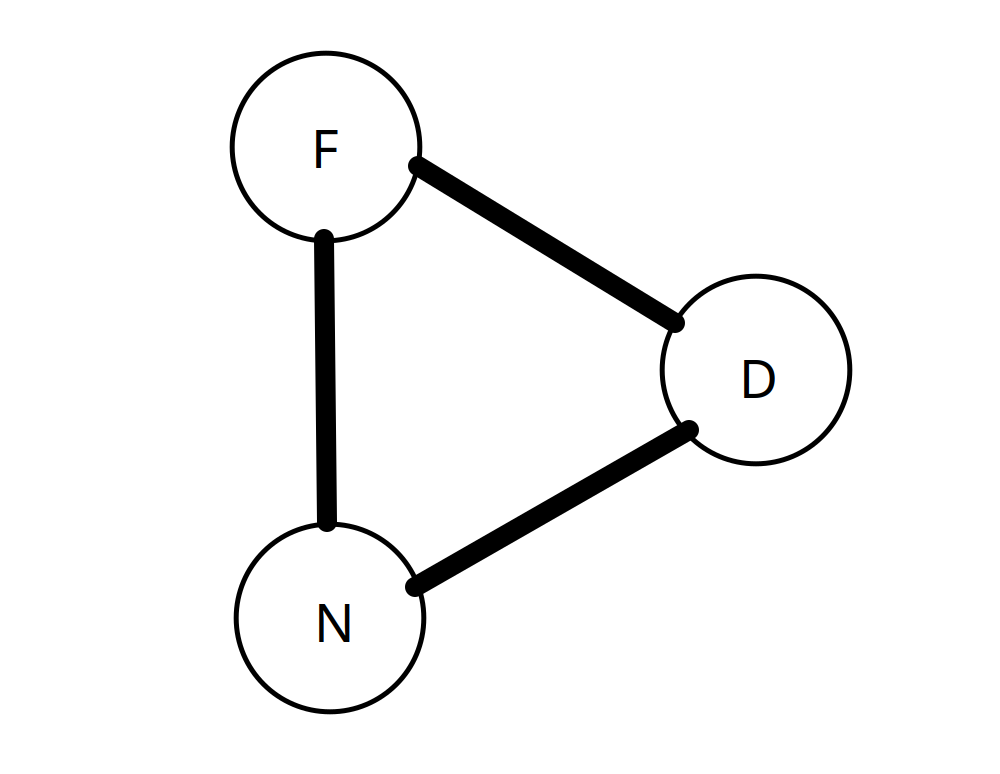
\includegraphics[scale=0.3]{Abbildungen/Pheromon_Dreieck.png}
		
		\caption{Experimentaufstellung\\
		in Anlehnung an \textit{Engelbrecht}~\cite{brecht2005fundamentals}}
		\label{subsec:Einfuehrung_In_Ameisenalgorithmen:Mathematische_Beschreibung_Der_Nahrungssuche_Von_Ameisen:fig:Pheromon_Dreieck}
	\end{figure}
	
	Weiter, in Anlehnung an \textit{Dorigo und Stützle}~\cite{dorigo2018ant} und wie in meiner Bachelorarbeit~\cite{FCM_2019} beschrieben, ergibt sich die Wahrscheinlichkeit, dass sich eine Ameise für das Begehen der Weges zwischen N und F entscheidet, aus der Gleichung~\ref{subsubsec:Einfuehrung_In_Ameisenalgorithmen:Mathematische_Beschreibung_Der_Nahrungssuche_Von_Ameisen:eq:Wahrscheinlichkeit_NF} und die Wahrscheinlichkeit, dass eine Ameise sich für das Begehen des Weges zwischen N und D entscheidet, aus Gleichung~\ref{subsubsec:Einfuehrung_In_Ameisenalgorithmen:Mathematische_Beschreibung_Der_Nahrungssuche_Von_Ameisen:eq:Wahrscheinlichkeit_ND}. Gleichung~\ref{subsubsec:Einfuehrung_In_Ameisenalgorithmen:Mathematische_Beschreibung_Der_Nahrungssuche_Von_Ameisen:eq:Verdunstung} beschreibt die Verdunstung des bereits vorhandenen Pheromons auf einem Weg nach dem eine Zeiteinheit verstrichen ist. Dabei ist \(\nu\) die Verdunstungskonstante, welche bestimmt, wie schnell Pheromon nach jedem Zeitschritt verdunstet, und \(\alpha\) ein Parameter, der bestimmt, wie viel Einfluss das auf einem Weg liegende Pheromon hat. Für Werte für \(\alpha\), nach \cite{dorigo2018ant}, gilt \(\alpha \in [0, 2]\). Wie viel Pheromon auf einem Weg liegt, also die Pheromoninformation, wird nach jedem Zeitschritt aktualisiert. Auf den Kanten, für die sich die Ameise entschieden hat, wird Pheromon abgelegt, gemäß Gleichung~\ref{subsubsec:Einfuehrung_In_Ameisenalgorithmen:Mathematische_Beschreibung_Der_Nahrungssuche_Von_Ameisen_eq:Pheromonablage}. 
	
	\begin{equation} \label{subsubsec:Einfuehrung_In_Ameisenalgorithmen:Mathematische_Beschreibung_Der_Nahrungssuche_Von_Ameisen:eq:Wahrscheinlichkeit_NF}
		prob_{NF} = \frac{\rho_{NF}^\alpha}{\rho_{NF}^\alpha+\rho_{ND}^\alpha}
	\end{equation}
	
	\begin{equation} \label{subsubsec:Einfuehrung_In_Ameisenalgorithmen:Mathematische_Beschreibung_Der_Nahrungssuche_Von_Ameisen:eq:Wahrscheinlichkeit_ND}
		prob_{ND} = \frac{\rho_{ND}^\alpha}{\rho_{ND}^\alpha+\rho_{NF}^\alpha}
	\end{equation}
	
	\begin{equation} \label{subsubsec:Einfuehrung_In_Ameisenalgorithmen:Mathematische_Beschreibung_Der_Nahrungssuche_Von_Ameisen:eq:Verdunstung}
		\rho_{XY} = (1-\nu)\cdot\rho_{XY}, ~ \nu \in [0,1), ~ XY \in \{NF, ND, DF\}
	\end{equation}
	
	\begin{equation} \label{subsubsec:Einfuehrung_In_Ameisenalgorithmen:Mathematische_Beschreibung_Der_Nahrungssuche_Von_Ameisen_eq:Pheromonablage}
		\rho_{XY} = \rho_{XY} + \Delta_{XY}
	\end{equation}
	
	Wie zu sehen, konstruiert das oben beschriebene Vorgehen eine Belegung der Knoten \(\{N, F, D\}\) so, dass die kürzeste Verbindung \(\{FN\}\) als Ergebnis entsteht, \(\{D\}\) also nicht begangen wird. Wie in meiner Bachelorarbeit~\cite{FCM_2019} beschrieben, kann beobachtet werden, dass die Orte N, F und D nur begangen und nicht begangen als Werte annehmen können. Damit ist das Problem die kürzeste Verbindung zu finden ein diskretes Problem, da die Werte, welche die Orte, verallgemeinert Variablen, annehmen können, abzählbar sind. Für das bis jetzt beschriebene Vorgehen wichtige Teilmenge von diskreten Problemen, sind Permutationsprobleme.
	
	\subsubsection{Permutationsprobleme} \label{subsubsec:Einfuehrung_In_Ameisenalgorithmen:Permuationsprobleme}
	
	In Anlehnung an meine Bachelorarbeit~\cite{FCM_2019}, kann ein Permutationsproblem definiert werden durch das Tupel \((\mathcal{G}, \pi, \Sigma, \mathcal{B}, f)\). Für den Grundraum \(\mathcal{G}\) glit hier \(\mathcal{G} = \{a_1, \dots, a_n\}, n \in \mathbb{N}_{>0}\), wobei die \(a_i\) beliebige Objekte sein können, die man ordnen kann. Die Permutation \(\pi: \Sigma \to \Sigma\) ordnet jedem Element \(a_i \in \Sigma, i \in \{1, \dots, n\}\) das korrespondierende Element \(a_{\pi(i)}\) zu. Für den Suchraum \(\Sigma\) gilt hier \(\Sigma = \{a_{\pi(1)}, \dots, a_{\pi(n)}\}\), wobei \(\{a_{\pi(1)}, \dots, a_{\pi(n)}\}\) jede Permutation der Grundmenge \(\{a_1, \dots, a_n\}\) ist. Die Menge an Beschränkungen, welche an die Ordnungen der \(a_i, i \in \{1, \dots, n\}\) oder Werte von \(f\) gestellt werden, werden mit \(\mathcal{B} = \{\mathcal{B}_1, \dots, \mathcal{B}_m\}, m \in \mathbb{N}_{>0}\) bezeichnet. Das Permutationsproblem ist unbeschränkt, wenn \(\mathcal{B} = \emptyset\) gilt, sonst ist es beschränkt. Die Zielfunktion \(f: \{a_{\pi(1)}, \dots, a_{\pi(n)}\} \to \mathbb{R}_{\geq 0}\) gibt die Güte einer Ordnung \(\{a_{\pi(1)}, \dots, a_{\pi(n)}\}\) der Objekte an. Eine Lösung \(s \in \Sigma\) ist eine Ordnung aller Elemente aus \(\Sigma\), welche konform ist mit den Beschränkungen \(\mathcal{B}\). Eine Lösung \(s_{opt}\) ist ein globales Optimum, wenn \(f(s_{opt}) \leq f(s) \, \forall s \in \Sigma\) gilt. Ein wichtiger Spezialfall eines Permutationsproblems ist das \ac{tsp}.
	
	\subsubsection{Traveling Salesperson Problem (TSP)} \label{subsubsec:Einfuehrung_In_Ameisenalgorithmen:Traveling_Salesperson_Problem_TSP}
	
	Das \ac{tsp}, nach \textit{Stützle et al.}~\cite{stutzle1999aco}, ist ein Permutationsproblem \((\mathcal{G}, \pi, \Sigma, d, \mathcal{B}, f)\) mit \(\mathcal{G} = \{a_i, \dots, a_n\}, n \in \mathbb{N}_{> 0}\), wobei beim \ac{tsp} die \(a_i\) die Städte sind und \(d: \mathbb{R} \times \mathbb{R} \to \mathbb{R}_{\geq 0}\) die Distanz zwischen zwei Städten ist. Da das \ac{tsp} keine Beschränkungen hat, gilt \(\mathcal{B} = \emptyset\). Die Permutation \(\pi\) gibt die Reihenfolge der Städte \(\{a_{\pi(1)}, \dots, a_{\pi(n)}\}\) und damit eine Rundreise an. Eine Rundreise ist eine Reise, bei der jede Stadt, außer der Startstadt, nur einmal besucht wird. Die Zielfunktion \(f\) gibt die Länge der Rundreise \(\{a_{\pi(1)}, \dots, a_{\pi(n)}\}\) an. Gesucht ist mindestens ein \(s_{opt} \in \Sigma, s_{opt} = \{a_{\pi(1)}, \dots, a_{\pi(n)}\}\), sodass gilt \(f(s_{opt}) \leq f(s) \, \forall s \in \Sigma\). Es ist also mindestens eine kürzeste Rundreise gesucht. Das \ac{tsp} war eines der Probleme, dass sich angeboten hat, um mit der ACO-Metaheuristik gelöst zu werden.
		
	\subsection{ACO-Metaheuristik nach \textit{Dorigo et al.}~\cite{dorigo1996ant}} \label{subsec:Grundlagen:ACO_-_Metaheuristik}
	
	Die ACO-Metaheuristik, nach \textit{Dorigo et al.}~\cite{dorigo1996ant}, steht für \textbf{A}nt \textbf{C}olony \textbf{O}ptimization-Metaheuristik und kann als Erweiterung der Konstruktion aus Abschnitt~\ref{subsubsec:Einfuehrung_In_Ameisenalgorithmen:Mathematische_Beschreibung_Der_Nahrungssuche_Von_Ameisen} gesehen werden, da sie auch als Tupel \((\Sigma, \mathcal{B}, \mathcal{E}, \Delta_c, \mathcal{M}_c, \eta, f, \mathcal{I}, \mathcal{S})\) angegeben werden kann. Dabei ist zwar \(\Sigma = G(V,E)\) aber \(V\) und \(E\) sind beliebig, genauso wie die Beschränkungen \(\mathcal{B}\). Weiter gilt \(|\mathcal{E}| = m, \, m \in \mathbb{N}\), anstatt \(|\mathcal{E}| = 1\). Die Menge des Pheromons \(\Delta\), welche die iterationsbeste Ameise auf die von ihr gewählten Kanten hinterlegt, wird problemabhängig gewählt. Die Pheromonmatrix \(\mathcal{M}\) kann größer sein als im Abschnitt~\ref{subsubsec:Einfuehrung_In_Ameisenalgorithmen:Mathematische_Beschreibung_Der_Nahrungssuche_Von_Ameisen} aber sie ist genauso aufgebaut und auch ihre Funktionalität ist die selbe. Auch die Verdunstungsmechanik aus Gleichung~\ref{subsubsec:Einfuehrung_In_Ameisenalgorithmen:Mathematische_Beschreibung_Der_Nahrungssuche_Von_Ameisen:eq:Verdunstung} wird beibehalten. Die problemabhängige Heuristik ist \(\eta\). Die Zielfunktion \(f\) kann auch beliebig formuliert werden, es bleibt jedoch gleich, dass mindestens eines ihrer globalen Minima gesucht wird. Das Initialisierungskriterium bleibt gleich, wie im Abschnitt~\ref{subsubsec:Einfuehrung_In_Ameisenalgorithmen:Mathematische_Beschreibung_Der_Nahrungssuche_Von_Ameisen}. Das Stoppkriterium \(\mathcal{S}\) kann frei gewählt werden.\hfill\newline
	
	Für die ACO-Metaheuristik angewandt auf das TSP kann \(\mathcal{B} = \max_{v_i, v_j \in V} d(v_i, v_j) \leq D\) sein, wobei \(D\) die maximale erlaubte Distanz zwischen zwei Städten ist, wenn die maximale Tankfüllung eines Transporters oder andere Beschränkungen berücksichtigt werden müssen, sonst gilt \(\mathcal{B} = \emptyset\). Die Anzahl der Ameisen ist \(|\mathcal{E}| = m\). Die Menge des Pheromons \(\Delta\), dass von der iterationsbesten Ameise abgelegt wird, ist in der Gleichung~\ref{subsec:ACO_-_Metaheuristik_Nach:eq:Delta} angegeben. Für das \ac{tsp} wird \(\eta\) in der Gleichung~\ref{subsec:ACO_-_Metaheuristik_Nach:eq:eta} angegeben, wobei \(d(v_i, v_j), v_i, v_j \in V\) die Distanz zwischen \(v_i\) und \(v_j\) ist.
	
	\begin{equation} \label{subsec:ACO_-_Metaheuristik_Nach:eq:Delta}
		\Delta_{ij} = \sum \limits_{k = 1}^m \frac{1}{f(s)}, (ij) \in s
	\end{equation}
	
	Dabei ist \(f\) die im Abschnitt~\ref{subsubsec:Einfuehrung_In_Ameisenalgorithmen:Traveling_Salesperson_Problem_TSP} definierte Zielfunktion, welche die Länge der Rundreise \(s\) wiedergibt. Wie zu sehen, ist die Menge des auf einer Kante \((i,j)\) hinterlegten Pheromons größer, je kürzer die Rundreise \(s\) ist, in der die Kante \((i,j)\) vorkommt.
	
	\begin{equation} \label{subsec:ACO_-_Metaheuristik_Nach:eq:eta}
		\eta_{ij} = \frac{1}{d(v_i, v_j)} \, \, \text{für zwei Knoten} \, v_i, v_j \in V
	\end{equation}
	
	Wie in \textit{Dorigo et al.}\cite{dorigo1996ant} beschrieben werden bei der Anwendung der ACO-Metaheuristik auf das TSP die Gleichungen \ref{subsubsec:Einfuehrung_In_Ameisenalgorithmen:Mathematische_Beschreibung_Der_Nahrungssuche_Von_Ameisen:eq:Wahrscheinlichkeit_NF} und \ref{subsubsec:Einfuehrung_In_Ameisenalgorithmen:Mathematische_Beschreibung_Der_Nahrungssuche_Von_Ameisen:eq:Wahrscheinlichkeit_ND} zuerst zur Gleichung~\ref{subsec:ACO_-_Metaheuristik_Nach:eq:Probabilistik_Rule} erweitert, wobei \(V'\) die Menge der Städte ist, die noch nicht besucht wurden, danach zur Gleichung~\ref{subsec:ACO_-_Metaheuristik_Nach:eq:Extended_Probabilistik_Rule}. Dabei hat \(\alpha\) die selbe Funktion, wie in den Gleichungen \ref{subsubsec:Einfuehrung_In_Ameisenalgorithmen:Mathematische_Beschreibung_Der_Nahrungssuche_Von_Ameisen:eq:Wahrscheinlichkeit_NF} und \ref{subsubsec:Einfuehrung_In_Ameisenalgorithmen:Mathematische_Beschreibung_Der_Nahrungssuche_Von_Ameisen:eq:Wahrscheinlichkeit_ND} und \(\beta\) ist ein Parameter, der bestimmt, wie viel Einfluss die Heuristik \(\eta\) hat. Die Gleichung~\ref{subsec:ACO_-_Metaheuristik_Nach:eq:Extended_Probabilistik_Rule} ist schließlich die Gleichung, welche beim Algorithmus~\ref{subsec:ACO_Metaheuristik:alg:ACO} im Schritt \glqq CreateSolution(ant)\grqq{} verwendet wird. In diesem Schritt wird eine Ameise zunächst auf einen zufällig ausgewählten Knoten gesetzt und von diesem Knoten aus wird dann mithilfe der Gleichung~\ref{subsec:ACO_-_Metaheuristik_Nach:eq:Extended_Probabilistik_Rule} der nächste Knoten gewählt. Dies wird solange wiederholt, bis \(V' = \emptyset\) gilt. \hfill\newline
	
	\begin{equation} \label{subsec:ACO_-_Metaheuristik_Nach:eq:Probabilistik_Rule}
		´prob_{ij} = \frac{\rho_{ij}}{\sum\limits_{v \in V'} \rho_{iv}}
	\end{equation}
	
	\begin{equation} \label{subsec:ACO_-_Metaheuristik_Nach:eq:Extended_Probabilistik_Rule}
		extend\_prob_{ij} = \frac{\rho_{ij}^{\alpha} \cdot \eta_{ij}^{\beta}}{\sum\limits_{v \in V'} \rho_{iv}^{\alpha} \cdot \eta_{iv}^{\beta}}
	\end{equation}
	
	Als Letztes fällt noch auf, dass \glqq UpdatePheromoneInformation\grqq{}, gegeben eine \(n \times n\)-Matrix, da jeder Matrixeintrag aktualisiert werden muss, \(\mathcal{O}(n^2)\) Schritte braucht, was bei großen Problemen viel Zeit verbraucht. Dies wurde durch \textit{Guntsch und Middendorf}~\cite{guntsch2002population}, mit der Weiterentwicklung der ACO-Metaheuristik zu der PB-ACO-Metaheuristik, verbessert.
	
	\begin{algorithm}
		
		\caption{ACO-Metaheuristik angewandt auf das TSP}\label{subsec:ACO_Metaheuristik:alg:ACO}
		
		\begin{algorithmic}[1]
			
			\Repeat
			
				%\State test
				\For {\(ant \in \mathcal{E}\)}
				
					\State CreateSolution(ant)
				
				\EndFor
				
				\State UpdatePheromoneInformation(\(\mathcal{M}\))
			
			\Until {\(\mathcal{S}\) fulfilled}
			
		\end{algorithmic}
		
	\end{algorithm}
	
	\subsection{Weiterentwicklung der ACO-Metaheuristik zu der PB-ACO-Metaheuristik} \label{subsec:Weiterentwicklung_Der_ACO_Metaheuristik_Zu_Der_P_-_ACO_Metaheuristik}
	
	Die folgende Beschreibung ist nach \textit{Guntsch und Middendorf}~\cite{guntsch2002population} und in Anlehnung an meine Bachelorarbeit~\cite{FCM_2019}.\hfill\newline
	
	PB-ACO steht für \textbf{P}opulation \textbf{B}ased-ACO-Metaheuristik. Die Unterschiede zu ACO sind, dass in PB-ACO die Pheromoninformation nicht mehr in einer stetigen \(n \times n\)-Pheromonmatrix \(\mathcal{M}\), sondern in einer diskreten \(n \times n\)-Pheromonmatrix \(\mathcal{M}_d\) gespeichert wird. Die Matrix \(\mathcal{M}_d\) ist diskret, da ihre Elemente nur endlich viele Werte annehmen können. In PB-ACO wird auch zudem eine Liste \(\mathcal{P}\) der Länge \(k, k \in \mathbb{N}\), von Lösungen mitgeführt, wobei in \cite{guntsch2002population} für das \ac{tsp} gilt \(k \in \{1, 5, 25\}\). Die in \(P\) gespeicherten Lösungen werden als Population interpretiert, daher \glqq PB-ACO\grqq{} als Name für diese Erweiterung von \glqq ACO\grqq. Demnach können wir, angelehnt an ACO, die PB-ACO-Metaheuristik als Tupel \((\Sigma, \mathcal{B}, \mathcal{E}, \Delta_d, \mathcal{M}_d, \mathcal{P}, \eta, f, \mathcal{I}, \mathcal{S})\) angeben. Nach \cite{guntsch2002population}, gilt für das \ac{tsp}, \(|\mathcal{E}| = 10\). Dabei wird in \textit{Guntsch und Middendorf}~\cite{guntsch2002population} die Liste der Populationen nach dem Prinzip \glqq first in last out\grqq{} befüllt. Bei diesem Prinzip wird, nachdem die Liste \(\mathcal{P}\) zunächst mit \(k\) Lösungen befüllt wurde, wenn eine neue Lösung generiert wird, die älteste Lösung entfernt, die verbleibenden Lösungen um eine Stelle nach hinten verschoben und die neue Lösung an den ersten Platz in der Liste \(\mathcal{P}\) gespeichert. Ein anderes Prinzip \(\mathcal{P}\) zu verwalten ist das \glqq best in worst out\grqq{} Prinzip. Dieses Prinzip wird im Abschnitt~\ref{subsec:Ameisenalgorithmen_Mit_Einem_Stetigen_Loesungsarchiv} erläutert. Das Befüllen von \(\mathcal{P}\) mit \(k\) Lösungen und dem folgenden Aufbau von \(\mathcal{M}_d\) ist hier die Initialisierungsmethode \(\mathcal{I}\). Ein weiterer Unterschied ist, dass die Pheromonmatrix \(\mathcal{M}_d\) nicht mehr beliebig viel Pheromoninformation enthält, wie \(\mathcal{M}\), sondern jedes Element nur \(k + 1\) verschiedene Werte annehmen kann, wodurch \(\mathcal{M}_d\) diskret ist. Ferner muss bei PB-ACO nicht mehr jedes Element der Pheromonmatrix \(\mathcal{M}_d\) bei jeder Iteration betrachtet werden. Nur die Elemente von \(\mathcal{M}_d\), welche in der neuen Lösung, welche in \(\mathcal{P}\) aufgenommen wird, vorkommen und die in der alten Lösung vorkommen, welche aus \(\mathcal{P}\) entfernt wird, und damit verändert werden, müssen betrachtet werden. Beides braucht \(n, n \in \mathbb{N}\) Schritte, also insgesamt \(2n\) Schritte. Damit braucht das Pheromonupdate statt \(\mathcal{O}(n^2)\) Zeit, nur \(\mathcal{O}(n)\), wie in \textit{Guntsch und Middendorf}~\cite{guntsch2002population} beschrieben.\hfill\newline
	
	Genauer, nach \cite{guntsch2002population} und \cite{FCM_2019}, seien \(\Delta > 0\), \(\Delta\) konstant, \(\rho_0 = 1/(n - 1)\). Dann werden die Elemente der Pheromonmatrix \(\mathcal{M}_d\) gemäß Gleichung~\ref{subsec:Weiterentwicklung_Der_ACO_Metaheuristik_Zu_Der_P_-_ACO_Metaheuristik:eq:Pheromone_Initialization} initialisiert. Nach \cite{guntsch2002population} gilt weiter für das \ac{tsp} für die Gleichung~\ref{subsec:ACO_-_Metaheuristik_Nach:eq:Extended_Probabilistik_Rule}, \(\alpha = 1\) und \(\beta = 5\). Die Elemente von \(\mathcal{M}_d\) werden dann, wie in Gleichung~\ref{subsec:Weiterentwicklung_Der_ACO_Metaheuristik_Zu_Der_P_-_ACO_Metaheuristik:eq:Pheromone_Update} dargestellt, aktualisiert. Dabei darf, wie zuvor, nur die iterationsbeste Ameise Pheromon legen. Die Tatsache, dass jedes Element von \(\mathcal{M}_d\) nur \(k + 1\) verschiedene Werte annehmen kann, ergibt sich daraus, dass, auf der einen Seite, jedes Element mindestens aus dem Initialisierungswert \(\rho_0\) besteht und, auf der anderen Seite, nur Vielfache von \(\Delta\) hinzugefügt werden können und das nur maximal \(k\)-Mal, da die Menge an Pheromon, welches die iterationsbeste Ameise ablegen kann, konstant \(\Delta\) ist und die Population der Ameisen \(\mathcal{P}\), nach Initialisierung, konstant die Größe \(k\) hat. Somit kann eine Kante \((i,j)\) nur maximal in \(k\) Lösungen vorkommen und damit ergibt sich, dass auf einer Kante nur \(k + 1\) verschiedene Mengen an Pheromon liegen können. Dies wird nochmal in der Gleichung~\ref{subsec:Weiterentwicklung_Der_ACO_Metaheuristik_Zu_Der_P_-_ACO_Metaheuristik:eq:Different_Pheromone_Values} verdeutlicht.
	
	\begin{equation} \label{subsec:Weiterentwicklung_Der_ACO_Metaheuristik_Zu_Der_P_-_ACO_Metaheuristik:eq:Pheromone_Initialization}
			(m_{ij})_{i,j = 1, \dots, n} = (\rho_{ij})_{i,j = 1, \dots, n} = \rho_0;
	\end{equation}
	
	\begin{equation} \label{subsec:Weiterentwicklung_Der_ACO_Metaheuristik_Zu_Der_P_-_ACO_Metaheuristik:eq:Pheromone_Update}
		\rho_{ij} = \rho_{ij} + \Delta
	\end{equation}
	
	\begin{equation} \label{subsec:Weiterentwicklung_Der_ACO_Metaheuristik_Zu_Der_P_-_ACO_Metaheuristik:eq:Different_Pheromone_Values}
		\rho_0 \leq \rho_{ij} \leq \rho_0 + k \cdot \Delta
	\end{equation}
	
	Schließlich kann festhalten werden, dass die Population \(\mathcal{P}\) als Lösungsarchiv interpretieren werden kann, mit dessen Hilfe neue Lösungen konstruiert werden können, da in \(\mathcal{P}\) die Pheromoninformation implizit gegeben ist. Darauf aufbauend wird in den folgenden Algorithmen in dieser Arbeit auf eine Pheromonmatrix verzichtet, da diese, gegeben \(\mathcal{P}\), überflüssig in diesen Algorithmen ist.
	
	\subsection{Alternative Verwaltung für ein Lösungsarchiv} \label{subsec:Alternative_Verwaltungen_Fuer_Ein_Loesunsarchiv}
	
	Ein anderes Prinzip ein Lösungsarchiv zu verwalten ist das \glqq best in worst out\grqq{} Prinzip. Bei diesem Prinzip, wie in meiner Bachelorarbeit~\cite{FCM_2019} beschrieben, wird eine Lösung nach ihrer Güte in das Lösungsarchiv einsortiert. Ist die Güte der neu generierte Lösung schlechter als die Güte aller Anderen im Archiv, wird sie ignoriert. Ist die Güte der neuen Lösung besser als bei einer Anderen, wird die letzte Lösung im Archiv gelöscht und alle Lösungen, die schlechter sind, als die neue Lösung, sofern diese existieren, wandern um eine Position im Archiv nach unten. Wird dieses Verwaltungsprinzip verwendet, legt es den Selektionsdruck von den Ameisen auf das Archiv, weswegen in den folgenden Algorithmen in dieser Arbeit gilt \(|\mathcal{E}| = 2\), wie im Abschnitt~\ref{subsec:ACO_R} oder \(|\mathcal{E}| = 1\), wie in den Abschnitten \ref{subsec:ACO_R_-_simple} und \ref{subsec:ACO_R_-_very_-_simple}. Dieses Verwaltungsprinzip wird in allen folgenden Algorithmen in dieser Arbeit verwendet. 
	
	\subsection{Ameisenalgorithmen mit einem stetigen Lösungsarchiv} \label{subsec:Ameisenalgorithmen_Mit_Einem_Stetigen_Loesungsarchiv}
	
	Wie in meiner Bachelorarbeit~\cite{FCM_2019} und im Abschnitt~\ref{subsec:Weiterentwicklung_Der_ACO_Metaheuristik_Zu_Der_P_-_ACO_Metaheuristik} beschrieben, kann man Pheromoninformation in einer diskreten Matrix speichern. Diese Matrix kann dann implizit als ein diskretes Lösungsarchiv interpretiert werden, was nur möglich ist, wenn Testfunktionen oder Probleme diskret sind. Um stetige Testfunktionen und Probleme zu lösen, bedarf es eines Archivs, welches stetige Einträge halten kann. Dies kann man erreichen, indem man ein Archiv erstellt, dass stetige Einträge halten kann, wie es vorher für diskrete Einträge gemacht wurde.\hfill\newline
	
	\subsection{Ameisenalgorithmen mit einem gemischten Lösungsarchiv}
	
	Da in dieser Arbeit die Art der Algorithmen, die getestet werden und die Art der Testfunktionen, die zum Testen benutzt werden, erweitert wird, muss auch der Begriff des Lösungsarchivs erweitert werden. Gegeben eine Funktion mit gemischten Variablen, wie in den Abschnitten \ref{subsubsec:Konstruierte_Probleme} und \ref{subsubsec:Coil_Spring_Design_Problem} und ein einfaches Lösungsarchiv mit \(n \in \mathbb{N}\) Einträgen, wie es im Abschnitt~\ref{subsec:Ameisenalgorithmen_Mit_Einem_Stetigen_Loesungsarchiv} definiert wurde, dann ist die einfachste Erweiterung für ein Lösungsarchiv, mehrere Lösungsarchive zu einem zusammengesetzten Lösungsarchiv zusammenzufassen. Dabei bilden die Einträge der Unterarchive an der Stelle \(i \in \{1, \dots, n\}, \, n \in \mathbb{N}\), eine Gesamtlösung. Zum Beispiel kann ein zusammengesetztes einfaches Lösungsarchiv \{\{'diskret': [1], 'stetig': [1.0,1.5]\}, \{'diskret': [2], 'stetig': [2.0,3.0]\}\} sein. Dann ist die \(2.\)te Lösung \{'diskret': [2], 'stetig': [2.0,3.0]\}.
	
	\subsection{Ameisenalgorithmen mit gemischten Lösungsarchiven in einer hierarchischen Struktur}
	
	Wie in \cite{kupfer2021hierarchical} beschrieben, werden bei einem hierarchischen Algorithmus die Ameisen in einer Baumstruktur angeordnet und die Anzahl der Archive wird von insgesamt 1 auf 3 pro Ameise erhöht. Ein Archiv für die letzte gefundene Lösung der Ameise, Eines für die bis dato beste gefundene persönliche Lösung der Ameise und Eines für die bis dato beste gefundene Lösung der Elternameise. Zusätzlich gibt es noch 1 weiteres Archiv, welches die bis dato insgesamt beste Lösung hält. Die Größe der Lösungsarchive schrumpft aber, von \(n = 100\) bei ACO\(_\mathbb{R}\)-VS~\cite{FCM_2019}, auf \(n = 1\). Dies ist notwendig, damit Lösungen entlang dem Baum wandern können, wie z.B. im HSPPBO-Schema, denn man kann Archive nur dann einfach vergleichen, wenn sie nur eine Lösung haben. Das Vergleichskriterium ist dann der Funktionswert der Fitnessfunktion.\hfill\newline
	
	Eine offene Forschungsfrage ist, wie mit Archiven in einer hierarchischen Struktur umgegangen werden kann, wenn sie mehr als 1 Lösung halten. Die einfachste Anordnung ist nach der Besten Lösung im Archiv zu ordnen. Die zweit einfachste Anordnung ist die Archive nach der Durchschnittsqualität der Lösungen zu sortieren. Eine komplexere Möglichkeit die Archive zu ordnen ist einen zusammengesetzten Term zu verwenden, wie in Gleichung~\ref{eq:Archiveguete} zu sehen. Dieser Term funktioniert sowohl für Archive, die Lösungen nach dem Prinzip \glqq first in last out\grqq{} speichern als auch für Archive, die Lösungen nach dem Prinzip \glqq best in worst out\grqq{} speichern. Im letzten Fall gilt \(s_1 = s_{opt}\).
	
	\begin{equation} \label{eq:Archiveguete}
		G"ute = c_1 \cdot f(s_1) + c_2 \cdot \frac{\sum_{i = 2}^n f(s_i)}{n - 1}
	\end{equation}
	
	Dabei sind \(c_1, c_2 \in \mathbb{R}\) Konstanten, \(s_{opt}\) ist die bis dato gefundene beste Lösung und \(n\) die Anzahl der Lösungen in den Archiven, wobei alle Archive die selbe Anzahl an Lösungen halten. In diesem Fall kann auf eine persönliche und globale beste Lösung verzichtet werden. Als Ausgangspunkt für weitere Forschung eignet sich mit der Beziehung \(c_1 + c_2 = 1\), \(c_1, c_2 \in [0,1]\) anzufangen. Später kann man allgemeiner verlangen, dass nur \(c_1, c_2 \in \mathbb{R}\) gilt. Als letzte Forschungsfrage können verschiedene Archive verschieden viele Lösungen halten.
	
	\subsection{Optimierungsprobleme} \label{sec:Optimierungsprobleme}
	
	Da wir, im Vergleich zu meiner Bachelorarbeit~\cite{FCM_2019}, in dieser Arbeit die Menge der betrachteten Testfunktionen und Probleme auf Testfunktionen und Probleme mit gemischten Variablen erweitern, bietet es sich an, eine abstraktere Definition von Optimierungsproblemen zu etablieren.\hfill\newline
	
	Wie an \cite{lin2015simple} angelehnt, wird ein Optimierungsproblem durch 4 Teile definiert. Diese sind der Suchraum \(\Sigma = \{\Sigma_1, \dots, \Sigma_n\}, n \in \mathbb{N}\), die Menge der abstrakten Variablen \(X = \{X_1, \dots, X_n\}, n \in \mathbb{N}\), die Beschränkungen an die Variablen \(\mathcal{B} = \{\mathcal{B}_1, \dots, \mathcal{B}_n\}, n \in \mathbb{N}\) und eine Fitness- bzw. Zielfunktion \(f: \Sigma \to \mathbb{R}^+\), die jeder Lösung \(s \in \Sigma\) einen Wert \(f(s) > 0\) zuordnet, wobei eine Lösung \(s \in \Sigma\) das Belegen aller Variablen \(X_i\) mit den Werten aus \(\Sigma_i\) ist, sodass die Werte den Beschränkungen \(\mathcal{B}_i\) genügen, \(i \in \{1, \dots, n\}\). Damit kann ein Optimierungsproblem definiert werden als das Tupel \((\Sigma, X, \mathcal{B}, f)\). Wenn \(\mathcal{B} = \emptyset\), dann ist das Problem unbeschränkt, sonst ist es beschränkt.\hfill\newline
	
	Eine Population \(\mathcal{P}\) besteht aus mindestens einer Lösung \(s \in \Sigma\). Alle Lösungen \(s \in \Sigma\), die auch in einer Population \(\mathcal{P}\) sind, werden durch \(\Sigma|\mathcal{P}\) beschrieben. Darauf aufbauend, gegeben eine Population \(\mathcal{P}\), beschreibt \(\Sigma|\mathcal{P}_i, i \in \{1, \dots, n\}\), alle Werte in \(\Sigma\) an der Stelle \(i\), die auch in \(\mathcal{P}\) an der Stelle \(i\) auftreten.\hfill\newline
	
	Eine Lösung \(s_{opt}\) heißt Optimum, wenn gilt \(f(s_{opt}) \leq f(s) \, \forall s \in \Sigma\). Ein Optimierungsproblem kann mehr als ein \(s_{opt}\) haben. Das Ziel eines Optimierungsproblems ist mindestens ein \(s_{opt}\) zu finden.\hfill\newline
	
	Mit dieser Definition kann beispielhaft der Suchraum und die Variablen für das \acl{csd} angegeben werden. Der Suchraum ist \(\Sigma = \{\mathbb{R}, \mathbb{O}, \mathbb{N}_{>0}\}\) und die Variablen sind \(X = \{D, d, N\}\). \(\mathbb{O}\) ist die Menge aller rationalen ordinalen Zahlen. Es ist die Menge der rationalen Zahlen \(\mathbb{Q}\) ohne eine Ordnungsrelation. \(D\) ist eine stetige Variable, \(d\) ist ordinal und N ist natürlich, wobei die Beschränkungen \(D \in \{3 \cdot d_{min}, 3.0\}\), \(d \in \{d_{min}, \dots, 0.5000\}\) und \(N \in \{1, \dots, 70\}\) gelten. Die Beschränkung \(d_{min}\) wird im Abschnitt~\ref{subsubsec:Coil_Spring_Design_Problem} zum \ac{csd} angegeben.
	
	\subsection{ACO\(_{\mathbb{R}}\)} \label{subsec:ACO_R}
	
	In Anlehnung an \textit{Socha und Dorigo}~\cite{socha2008ant} und wie in meiner Bachelorarbeit~\cite{FCM_2019} beschrieben, baut der ACO\(_{\mathbb{R}}\) Algorithmus auf einem stetigen Lösungsarchiv \(\mathcal{P}_c\) der Größe \(k\) auf. Auf eine Pheromonmatrix und damit auf Pheromon, sowie eine problemabhängige Heuristik wird verzichtet. Demnach kann ACO\(_{\mathbb{R}}\) als Tupel \((\Sigma, \mathcal{B}, \mathcal{E}, \mathcal{P}_c, f, \mathcal{I}, \mathcal{S})\) angegeben werden. In \cite{socha2008ant} gilt \(|\mathcal{E}| = 2\), \(|\mathcal{P}_c| = k = 50\).\hfill\newline
	
	Die Initialisierungsmethode \(\mathcal{I}\) ist auch hier das Füllen von \(\mathcal{P}_c\) mit Lösungen, wie bei PB-ACO. Aber das Stoppkriterium ist problemabhängig. So kann z.B. \(|f - f^*| < \varepsilon, \varepsilon = 10^{-10}\) sein, wie in Abschnitt~\ref{subsec:Stetige_Testfunktionen}, wobei \(f^*\) das bekannte Optimum einer Testfunktion ist und \(f\) der Momentane Funktionswert, den der Lösungsalgorithmus gefunden hat.\hfill\newline
	
	Die Veränderung von PB-ACO zu ACO\(_{\mathbb{R}}\), um stetige Testfunktionen und Probleme lösen zu können, transformiert die Lösungskonstruktion aus Gleichung~\ref{subsec:ACO_-_Metaheuristik_Nach:eq:Extended_Probabilistik_Rule} zur Gleichung~\ref{subsec:ACO_R:eq:Gauss_-_Kern_In_i_-_th_Dimension}. Und es wird nicht mehr betrachtet wie wahrscheinlich das Wandern entlang einer Kante \((i,j)\) ist, sondern es wird im \(i\)-ten Konstruktionsschritt ein Gauss-Kernel in der \(i\)-ten Dimension ausgewertet, wobei gilt \(i \in \{1, \dots, n\}, n \in \mathbb{N}\), und \(n\) ist sowohl die Dimension der Testfunktion, als auch die Anzahl der Konstruktionsschritte, die jede Ameise pro Iteration macht.\hfill\newline¨
	
	\begin{equation} \label{subsec:ACO_R:eq:Gauss_-_Kern_In_i_-_th_Dimension}
		G^i=\sum_{l=1}^{k} \omega_l g^i_l(x)=\sum_{l=1}^{k} \omega_l \frac{1}{ \sigma^i_l \sqrt{2\pi} }e^{-\frac{(x-\mu^i_l)^2}{2 {\sigma^i_l}^2}}, ~  i \in \{1, ..., n\}
	\end{equation}
	
	\noindent Weiter, in Anlehnung an \textit{Socha und Dorigo}~\cite{socha2008ant} gilt für die Vektoren \(\omega\) , \(\mu\) und \(\sigma\), dass ihre Kardinalität gleich der Kardinalität von \(\mathcal{P}\) ist, also gilt \(|\omega| = |\mu| = |\sigma| = |\mathcal{P}| = k = 50\). Die Elemente der Parametervektoren \(\omega\) , \(\mu\) und \(\sigma\) werden in den Gleichungen \ref{subsec:ACO_R:eq:mu}, \ref{subsec:ACO_R:eq:omega} und \ref{subsec:ACO_R:eq:sigma} berechnet. Dabei gilt, dass \(n\) die Anzahl der Dimensionen der Testfunktion und \(i\) der Konstruktionsschritt ist. Weiter ist \(s^i_j\) die \(i\)-te Variable der \(j\)-ten Lösung. Der Parametervektor \(\omega\) unterscheidet sich von \(\mu\) und \(\sigma\) darin, dass er nicht zur Erzeugung der nächsten Lösung benutzt wird, sondern er jeder bereits vorhandenen Lösung im Lösungsarchiv \(\mathcal{P}_c\) ein Gewicht \(\omega_l\) zuordnet, welches dazu benutzt wird mithilfe der Gleichung~\ref{subsec:ACO_R:eq:Probability_Distribution} eine Wahrscheinlichkeitsverteilung aufzubauen. Unter Anwendung dieser Wahrscheinlichkeitsverteilung wird dann die \(l\)-te Gaußfunktion gewählt.\hfill\newline
	
	Der Term in Gleichung~\ref{subsec:ACO_R:eq:sigma} wird in \textit{Socha und Dorigo}~\cite{socha2008ant} als Standardabweichung bezeichnet, auch wenn in diesem Term keine Wurzel vorhanden ist. Dies wird so verstanden, dass der Term zwar aus mathematischer Sicht keine Standardabweichung ist aber als Standardabweichung für den Algorithmus interpretiert wird, da in der Gleichung~\ref{subsec:ACO_R:eq:Gauss_-_Kern_In_i_-_th_Dimension} nach einer Standardabweichung verlangt wird.
	
	\begin{equation} \label{subsec:ACO_R:eq:mu}
		\mu = \{ \mu^i_1, ...,\mu^i_k \} = \{ s^i_1, ..., s^i_k \}, ~ i \in \{1, ..., n\}
	\end{equation}
	
	\begin{equation} \label{subsec:ACO_R:eq:omega}
		\omega_l = \frac{1}{qk\sqrt{2\pi}}e^{-\frac{(l-1)^2}{2q^2k^2}}, ~ 
		l \in \{1, ..., k\}
	\end{equation}
	
	\begin{equation} \label{subsec:ACO_R:eq:sigma}
		\sigma^i_l=\xi \sum_{e=1}^{k} \frac{|s^i_e-s^i_l|}{k-1}, ~ l \in \{1, ..., k\}, ~ i \in \{1, ..., n\}
	\end{equation}
	
	\begin{equation} \label{subsec:ACO_R:eq:Probability_Distribution}
		p_l = \frac{\omega_l}{\sum_{r=1}^{k} \omega_r}, ~ 
		l \in \{1, ..., k\}
	\end{equation}
	
	Nachdem die Parametervektoren berechnet wurden, wird im Konstruktionsschritt \(i\) die Gaußfunktion \(g^i_l\) ausgewertet, was durch einen Zufallszahlengenerator, der Zufallszahlen aus einer parametrisierten Normalverteilung erzeugt, passieren kann.\hfill\newline
	
	Der Parameter \(q\) steuert, wie stark bessere Lösungen im Archiv bei der Konstruktion einer neuen Lösung bevorzugt werden. Je kleiner \(q\), desto stärker werden bessere Lösungen bevorzugt. Der Parameter \(\xi\) steuert, wie schnell der Algorithmus konvergiert. Je größer \(\xi\), desto langsamer konvergiert der Algorithmus. In \cite{socha2008ant} gilt \(q = 10^{-4}\), \(\xi = 0.85\).\hfill\newline
	
	\subsection{ACO\(_{\mathbb{R}}\)-simple} \label{subsec:ACO_R_-_simple}
	
	Wie in meiner Bachelorarbeit~\cite{FCM_2019} beschrieben, entstand der ACO\(_{\mathbb{R}}\)-simple Algorithmus durch eine Vereinfachung des ACO\(_\mathbb{R}\) Algorithmus. Der ACO\(_{\mathbb{R}}\)-simple Algorithmus nutzt das Lösungsarchiv auch wie ACO\(_{\mathbb{R}}\), jedoch setzt er die vorhandenen Lösungen auf eine einfachere Weise zu einer neuen Lösung zusammen -- deswegen simple, also einfach.\hfill\newline
	
	Die vier Konzepte, die aus ACO\(_{\mathbb{R}}\) übernommen wurden, ist die Verwendung eines Lösungsarchivs \(\mathcal{P}_c\), die Zuweisung jeder Lösung im Archiv eines Gewichts \(w_i\), dass mit der Gleichung~\ref{subsec:ACO_R_-_simple:eq:omega} berechnet und zum Aufbau einer Wahrscheinlichkeitsverteilung mithilfe der Gleichung~\ref{subsec:ACO_R_-_simple:eq:Probability_Distribution} benutzt wird und somit wie eine Lösung \(s_i\) aus dem Archiv gewählt wird, die Art wie die Abweichung in Gleichung~\ref{subsec:ACO_R_-_simple:eq:Linear_Deviation} berechnet wird, sowie die Verwendung der Parameter \(q\) und \(\xi\). Bei der Berechnung der Abweichung in Gleichung~\ref{subsec:ACO_R_-_simple:eq:Linear_Deviation} wird aber, aufgrund der Art und Weise wie die Abweichung später verwendet wird, explizit die lineare Abweichung gewollt.\hfill\newline
	
	Im Gegensatz zu ACO\(_\mathbb{R}\) gilt in ACO\(_{\mathbb{R}}\)-very-simple aber \(|\mathcal{P}| = k = 100\), \(q = 0.95\) und \(\xi = 0.95\). Die Archivgröße wurde verdoppelt, da der Algorithmus einfacher ist als ACO\(_\mathbb{R}\) und damit eine größere Archivgröße ACO\(_{\mathbb{R}}\)-very-simple erlaubt auch vom momentanen Bestwert weiter entferntere Lösungen im Suchraum zu erforschen. Das ist auch der selbe Grund, wieso \(q = 0.95\) gesetzt wurde. Auf der anderen Seite wurde \(\xi = 0.95\) gesetzt, damit das Suchintervall in Gleichung~\ref{subsec:ACO_R_-_simple:eq:Suchintervall} möglichst erhalten bleibt. Es gab auch die Möglichkeit \(\xi = 1.0\) zu setzen aber im Sinne der Einfachheit wurde \(q = \xi = 0.95\) gesetzt. Im Bestreben nach Einfachheit wurde auch \(|\mathcal{E}| = 1\) gesetzt, da der Selektionsdruck, der durch das Verwalten des Lösungsarchivs nach dem \glqq best in worst out\grqq Prinzip entsteht, für ausreichend gehalten wurde. Demnach kann ACO\(_{\mathbb{R}}\)-simple als Tupel \((\Sigma, \mathcal{B}, \mathcal{E}, \mathcal{P}_c, f, \mathcal{I}, \mathcal{S})\) angeben werden. Der größte Unterschied zu ACO\(_\mathbb{R}\) liegt aber darin wie ACO\(_{\mathbb{R}}\)-simple eine neue Lösung erzeugt. Denn nachdem die lineare Abweichung in jeder Dimension \(d, d \in \{1, \dots, n\}\) der \(n\)-dimensionalen Testfunktion/des \(n\)-dimensionalen Problems in Gleichung~\ref{subsec:ACO_R_-_simple:eq:Linear_Deviation} berechnet wurde, wird nur noch ein Intervall in Gleichung~\ref{subsec:ACO_R_-_simple:eq:Suchintervall} in jeder Dimension \(d, d \in \{1, \dots, n\}\) der Testfunktion/des Problems mithilfe der linearen Abweichung aufgebaut und dann wird aus jedem der Intervalle ein zufälliger Punkt als Komponente der neuen Lösung gewählt.
	
	\begin{equation} \label{subsec:ACO_R_-_simple:eq:omega}
		\omega_i = \frac{1}{qk\sqrt{2\pi}}e^{-\frac{(i-1)^2}{2q^2k^2}}, ~ 
		i \in \{1, ..., k\}
	\end{equation}
	
	\begin{equation} \label{subsec:ACO_R_-_simple:eq:Probability_Distribution}
		p_i=\frac{w_i}{\sum_{j=1}^{n} w_j}, ~  i \in \{1, ..., k\}
	\end{equation}
	
	\begin{equation} \label{subsec:ACO_R_-_simple:eq:Linear_Deviation}
		\delta_d = \xi\sum_{j=1}^{k} \frac{|s_{j\_d}-s_{i\_d}|}{k-1}, ~ j \in \{1, ..., k\}, ~ d \in \{1, ..., n\}
	\end{equation}
	
	\begin{equation} \label{subsec:ACO_R_-_simple:eq:Suchintervall}
		[s_d - \delta_d, s_d + \delta_d], ~ d \in \{1, ..., n\}
	\end{equation}
	
	\noindent Die Standardeinstellungen der Parameter sind, wie in Tabelle~\ref{ACO_R_simple_Parametereinstellungen} zu sehen ist.
	
	\begin{table}[H]
		\fontsize{10pt}{12pt}
		
		\caption{Parametereinstellungen ACO\(_{\mathbb{R}}\)-simple}
		\label{ACO_R_simple_Parametereinstellungen}
		
		\begin{tabularx}{\textwidth}{l|r|r}
			
			\rule{4.6cm}{0.4pt} & \rule{4.6cm}{0.4pt}& \rule{4.6cm}{0.4pt}\\
			
			Parameter & Symbol & Wert\\
			
			\rule{4.6cm}{0.4pt} & \rule{4.6cm}{0.4pt}& \rule{4.6cm}{0.4pt}\\
			
			Anzahl der Ameisen & m & 1\\
			Konvergenzgeschwindigkeit & \(\xi\) & 0.95\\
			Lokalität der Suche & \textit{q} & 0.95\\
			Archivgröße & k & 100
			
			
		\end{tabularx}
		
	\end{table}
	
	\subsection{\acl{acorvs}} \label{subsec:ACO_R_-_very_-_simple}
	
	Wie in meiner Bachelorarbeit~\cite{FCM_2019} beschrieben, baut der Algorithmus \ac{acorvs} auf ACO\(_{\mathbb{R}}\)-simple auf, indem er ACO\(_{\mathbb{R}}\)-simple weiter vereinfacht -- deswegen very-simple, also sehr einfach. Jedoch sind die Algorithmen sich noch hinreichend ähnlich, dass \ac{acorvs} als Tupel \((\Sigma, \mathcal{B}, \mathcal{E}, \mathcal{P}_c, f, \mathcal{I}, \mathcal{S})\) angegeben werden kann. Die Vereinfachung besteht darin, dass, anstatt eine Lösung aus dem Archiv nach einer Wahrscheinlichkeitsverteilung auszuwählen, immer die erste und damit beste Lösung \(s_1\) im Archiv zur Lösungsgenerierung gewählt wird. Damit entfallen die Pendants zu den Gleichungen \ref{subsec:ACO_R_-_simple:eq:omega} und \ref{subsec:ACO_R_-_simple:eq:Probability_Distribution} und es kann direkt die Gleichung~\ref{subsec:ACO_R_-_very_-_simple:eq:interval} berechnet werden. Danach wird in \ac{acorvs}, genau wie in ACO\(_{\mathbb{R}}\)-simple, in jeder Dimension \(d, d \in \{1, \dots, n\}\) der \(n\)-dimensionalen Testfunktion/des \(n\)-dimensionalen Problems, mithilfe der Gleichung~\ref{subsec:ACO_R_-_very_-_simple:eq:interval}, ein Intervall aufgebaut und dann wird aus jedem dieser Intervalle ein zufälliger Punkt als Komponente der Lösung gewählt.
	
	\begin{equation} \label{subsec:ACO_R_-_very_-_simple:eq:Linear_Diviation}
		\delta_d = \xi\sum_{j=1}^{k} \frac{|s_{j\_d}-s_{1\_d}|}{k-1}, ~ j \in \{1, ..., k\}, ~ d \in \{1, ..., n\}
	\end{equation}
	
	\begin{equation} \label{subsec:ACO_R_-_very_-_simple:eq:interval}
		[s_d - \delta_d, s_d + \delta_d], ~ d \in \{1, ..., n\}
	\end{equation}
	
	\noindent Die Standardeinstellungen der Parameter sind, wie in Tabelle~\ref{ACO_R_very_simple_Parametereinstellungen} zu sehen ist.
	
	\begin{table}[H]
		\fontsize{10pt}{12pt}
		
		\caption{Parametereinstellungen \ac{acorvs}}
		\label{ACO_R_very_simple_Parametereinstellungen}
		
		\begin{tabularx}{\textwidth}{l|r|r}
			
			\rule{4.6cm}{0.4pt} & \rule{4.6cm}{0.4pt}& \rule{4.6cm}{0.4pt}\\
			
			Parameter & Symbol & Wert\\
			
			\rule{4.6cm}{0.4pt} & \rule{4.6cm}{0.4pt}& \rule{4.6cm}{0.4pt}\\
			
			Anzahl der Ameisen & m & 1\\
			Konvergenzgeschwindigkeit & \(\xi\) & 0.95\\
			Archivgröße & k & 100
			
			
		\end{tabularx}
		
	\end{table}
	
	\subsection{Erweiterung von \acl{acorvs} zu \acl{acorvsmv} für Probleme mit diskreten Variablen}
	
	Da ACO\(_\mathbb{R}\)-VS ursprünglich für Funktionsoptimierung von stetigen Testfunktionen/Problemen entwickelt wurde, muss die ACO\(_\mathbb{R}\)-VS-Metaheuristik für diskrete Testfunktionen/Probleme angepasst werden.\hfill\newline
	
	Um ACO\(_\mathbb{R}\)-VS anzupassen werden nicht-stetige Testfunktionen/Probleme als stetige Testfunktionen/Probleme behandelt. Das heißt, es wird mit nicht-stetigen Werten gerechnet als wären sie stetig. Es wird also bis zur Gleichung~\ref{subsec:ACO_R_-_very_-_simple:eq:interval} genauso verfahren, wie im Abschnitt~\ref{subsec:ACO_R_-_very_-_simple}, um einen neuen, stetigen Wert zu erhalten. Nachdem man einen neuen stetigen Wert gewonnen hat, betrachtet man die nicht-stetigen Werte zwischen denen der stetige Wert liegt und wählt dann als Ergebnis, den nicht-stetigen Wert, an dem der Stetige am nächsten liegt. Diese so gewonnen Erweiterung von \ac{acorvs} wird \acl{acorvsmv} oder kurz \ac{acorvsmv} genannt.\hfill\newline
	
	Schließlich wird \ac{acorvs} um eine Neustartstrategie erweitert. Der Algorithmus kann entweder eine fixe Anzahl an Neustarts ausführen oder adaptiv neu starten. Für die Neustartstrategie, bei welcher der Algorithmus eine fixe Anzahl neu startet, wird die Anzahl mit \(fixed = n\) angegeben. Es wurde \(n = 0\) gesetzt, um einen Kontrast zu der Neustartstrategie \(adaptvie\) zu haben. Wenn die Neustartstrategie \(adaptiv\) gewählt wurde, startet der Algorithmus neu, wenn eine Periode von \(\gamma\) Lösungen hintereinander sich um weniger als ein Threshold \(\varepsilon_{th}\) unterscheiden. Im Sinne der Einfachheit wurde als Start \(\gamma = 7\) und \(\varepsilon_{th} = 10^{-10}\) gesetzt. 
	
	\begin{table}[H]
		\fontsize{10pt}{12pt}
		
		\caption{Parametereinstellungen \ac{acorvsmv}}
		\label{subsec:Grundlagen:tab:ACO_R_VS_MV_Parametereinstellungen}
		
		\begin{tabularx}{\textwidth}{l|r|r}
			
			\rule{4.6cm}{0.4pt} & \rule{4.6cm}{0.4pt}& \rule{4.6cm}{0.4pt}\\
			
			Parameter & Symbol & Wert\\
			
			\rule{4.6cm}{0.4pt} & \rule{4.6cm}{0.4pt}& \rule{4.6cm}{0.4pt}\\
			n 			& n			 & 0\\
			Periode 	& \(\gamma\) & 7\\
			Threshold 	& \(\varepsilon_{th}\) & \(10^{-10}\)
			
		\end{tabularx}
		
	\end{table}
	
	\subsection{Erweiterung von ACO\(_\mathbb{R}\) zu ACO\(_\text{MV}\) für Probleme mit diskreten Variablen}
	
	Die Erweiterung von ACO\(_\mathbb{R}\) zu ACO\(_\text{MV}\) ist ähnlich zu der Erweiterung von \acl{acorvs} zu \acl{acorvsmv}. Wie in \textit{Socha}~\cite{socha2009ant} beschrieben, damit ACO\(_\text{MV}\) mit diskreten Variablen umgehen kann, rechnet ACO\(_\text{MV}\) mit den Indizes der diskreten Werte in Form von reellen Zahlen, anstatt mit den diskreten Werten selbst. Weiter rechnet ACO\(_\text{MV}\) wie ACO\(_\mathbb{R}\). Am Ende werden dann die gewonnen Werte für die diskreten Werte an die Indizes gerundet, die am nächsten an den neuen diskreten Werten liegen.
	
	\subsection{Vergleichsalgorithmen} \label{Grundlagen:Vergleichsalgorithmen}
	
	Neben dem Algorithmus ACO\(_\mathbb{R}\) selbst, gibt es noch drei Gruppen von Algorithmen, mit denen sich \ac{acorvs} und die Iterationen von \ac{acorvsmv} vergleichen. Die Algorithmen dieser Gruppen sind in den Abschnitten \ref{subsubsec:Grundlagen:Vergleichsalgorithmen:Alg_prob_Lernen}, \ref{subsubsec:Grundlagen:Vergleichsalgorithmen:Alg_verwandt_Ameisenalg} und \ref{subsubsec:Grundlagen:Vergleichsalgorithmen:Meta_-_Heuristiken_stetige_Probleme} vorgestellt.
	
	\subsubsection{Algorithmen, die probabilistisches Lernen einsetzen} \label{subsubsec:Grundlagen:Vergleichsalgorithmen:Alg_prob_Lernen}
	
	\paragraph{(1 + 1)-ES}\mbox{}\\
	
	Die folgende Beschreibung ist nach \textit{Rechenberg}~\cite{rechenberg1973evolutionsstrategie}.\hfill\newline

	ES steht für \textbf{E}volution \textbf{S}trategies. (1 + 1)-ES ist eines der ersten ES, die für Optimierung von stetigen Funktionen \(f\) vorgeschlagen wurden. In (1 + 1)-ES wird mit einem Elter (parent) begonnen und in jeder Iteration gibt es nur ein Kind (offspring), deswegen (1 + 1). Die zugrunde liegende Population besteht also, in jeder Generation \(g, g \in \{0, 1, 2, \dots\}\), nur aus dem Elter und dem Kind. Nach der Initialisierung des Elter \(x^{(g)}_{parent}\), wird das Kind \(x^{(g + 1)}_{offspring}\) in der Gleichung~\ref{subsubsubpar:Grundlagen:Vergleichsalgorithmen:1_und_1_-_ES:eq:Offspring} gewonnen, wobei \(I\) die Einheitsmatrix ist und \(\sigma\) die Verteilungsvarianz ist und als \glqq Step Size\grqq{} bezeichnet wird.
	
	\begin{equation} \label{subsubsubpar:Grundlagen:Vergleichsalgorithmen:1_und_1_-_ES:eq:Offspring}
		x^{(g + 1)}_{offspring} = z, \, z \sim \mathcal{N}(x^{(g)}_{parent}, \sigma^{(g)^2}I)
	\end{equation}
	
	 Weiter wird mit der Gleichung~\ref{subsubsubpar:Grundlagen:Vergleichsalgorithmen:eq:1_und_1_-_ES} verfahren und das so gewonnene Kind wird zum neuen Elter.
	
	\begin{equation} \label{subsubsubpar:Grundlagen:Vergleichsalgorithmen:eq:1_und_1_-_ES}
		x^{(g + 1)}_{offspring} =
			\begin{cases}
				x^{(g + 1)}_{offspring} &\text{, wenn } f(x^{(g + 1)}) \leq f(x^{(g)}_{parent})\\
				\\
				x^{(g)}_{parent} 		&\text{, sonst.}
			\end{cases}
	\end{equation}
	
	\paragraph{CSA-ES}\mbox{}\\
	
	Die folgende Beschreibung ist nach \textit{Ostermeier et al.}~\cite{ostermeier1994step}.\hfill\newline
	
	CSA-ES steht für \textbf{E}volutionary \textbf{S}trategy with \textbf{C}umulative \textbf{S}tep Size \textbf{A}daptation und ist eine Weiterentwicklung von (1 + 1)-ES. Die Weiterentwicklung besteht darin, dass die Step Size \(\sigma\) adaptiv ist und in Abhängigkeit des Weges, welcher von den letzten \(n, n \in \mathbb{N}\), Generationen gewählt wurde, geändert wird.
	
	\paragraph{CMA-ES}\mbox{}\\
	
	Die folgende Beschreibung ist nach \textit{Hansen und Ostermeier}~\cite{hansen2001completely}.\hfill\newline
	
	CMA-ES steht für \textbf{E}volutionary \textbf{S}trategy with \textbf{C}ovariance \textbf{M}atrix \textbf{A}daptation. Es ist die Weiterentwicklung von CSA-ES, bei der \(\sigma\) von einer Kovarianzmatrix beeinflusst wird.
	
	\paragraph{IDEA}\mbox{}\\
	
	Die folgende Beschreibung ist nach \textit{Bosman und Thierens}\cite{bosman2000continuous}.\hfill\newline
	
	IDEA steht für das IDEA-Framework, was wiederum für \textbf{I}terated \textbf{D}ensity Estimation \textbf{E}volutionaty \textbf{A}lgorithms-Framework steht. Algorithmen, die mit dem IDEA-Framework entworfen wurden, bauen probabilistische Modelle und schätzen Wahrscheinlichkeitsdichten, gegeben einiger Anfangspunkte.
	
	\paragraph{MBOA}\mbox{}\\
	
	Die folgende Beschreibung ist nach \textit{Očenášek und Schwarz}~\cite{ocenavsek2002estimation}.\hfill\newline
	
	MBOA steht für \textbf{M}ixed \textbf{B}ayesian \textbf{O}ptimization \textbf{A}lgorithm. Es ist die Weiterentwicklung von hBOA, das wiederum für \textbf{h}ierarchical \textbf{B}ayesian \textbf{O}ptimization \textbf{A}lgorithm steht. Nach \cite{pelikan2001bayesian} ist hBOA der erste Estimation of Distribution Algorithm (EDA), der Bayessche Netze mit Entscheidungsbäumen kombinierte. MBOA ist eine Erweiterung von hBOA, die auch mit gemischten Variablen, diskret und stetig, umgehen kann.
	
	\subsubsection{Algorithmen, die verwandt zu Ameisenalgorithmen sind} \label{subsubsec:Grundlagen:Vergleichsalgorithmen:Alg_verwandt_Ameisenalg}
	
	\paragraph{CACO}\mbox{}\\
	
	Die folgende Beschreibung ist nach \textit{Bilchev und Parmee}~\cite{bilchev1995ant}.\hfill\newline
	
	CACO steht für \textbf{C}ontinuous ACO. In CACO startet der Algorithmus mit einem zufälligen Punkt \(\mathcal{N}\) im Suchraum. Dieser Punkt wird \glqq Nest\grqq{} bezeichnet. Gute Lösungen werden als Vektoren, ausgehend vom Nest, gespeichert. Danach wird probabilistisch ein Vektor gewählt und sein Ende wird zum neuen Nest. Danach wird der Algorithmus wiederholt.
	
	\paragraph{API}\mbox{}\\
	
	Die folgende Beschreibung ist nach \textit{Monmarché et al.}~\cite{monmarche2000pachycondyla}.\hfill\newline
	
	API ist nach der \glqq Pachycondyla apicalis\grqq-Ameise benannt -- \glqq Pachycondyla \textbf{API}calis\grqq{} -- und der Algorithmus API ist der Nahrungssuche dieser Ameise nachempfunden. Dabei startet auch API mit einem zufälligen Punkt \(\mathcal{N}\), der Nest bezeichnet wird, im Suchraum. Ausgehend von \(\mathcal{N}\) etablieren \(n\) Ameisen Jagdgründe innerhalb eines Kreises um \(\mathcal{N}\) mit dem Radius \(R = 20 \, LE\), \(LE = L"angeneinheit\). In \cite{monmarche2000pachycondyla} wird \(n = 20\) gesetzt. Jeder Jagdgrund hat selbst einen Grenzkreis von \(r = 2 \, LE\). Jede Ameise kann sich \(p\) Jagdgründe merken. In \cite{monmarche2000pachycondyla} wird \(p = 2\) gesetzt. Jede Ameise führt dann eine Suche in einem von ihr gemerkten Jagdgründe aus. Wenn in einem Jagdgrund \(P\)-mal keine bessere Lösung, als die von der jeweiligen Ameise bis dato gefundene Lösung, gefunden wurde, wird der Jagdgrund vergessen. In der Wildnis gilt für die echten Ameisen \(1 \, LE = 1 \, Meter\). Nach \(T\) Iterationen, wobei in \cite{monmarche2000pachycondyla} \(T = 50\) gesetzt wird, wird das Nest \(\mathcal{N}\) an den bis dato besten gefunden Punkt gesetzt. Es wurde in \cite{monmarche2000pachycondyla} \(P = T\) gesetzt, damit ein Jagdgrund erst dann vergessen wird, wenn das Nest \(\mathcal{N}\) bewegt wird.
	
	\paragraph{CIAC}\mbox{}\\
	
	Die folgende Beschreibung ist nach \textit{Dréo and Siarry}~\cite{dreo2002new}.\hfill\newline
	
	CIAC steht für \textbf{C}ontinuous \textbf{I}nteracting \textbf{A}nt \textbf{C}olony. In CIAC kommunizieren die Ameisen auf zwei Wegen, indirekt über Pheromon und direkt über Nachrichten. Nachrichten bestehen wiederum aus zwei Komponenten, die Position des Senders und dem Funktionswert der Zielfunktion an seiner Position.
	
	\subsubsection{Metaheuristiken, die für stetige Testfunktionen adaptiert wurden} \label{subsubsec:Grundlagen:Vergleichsalgorithmen:Meta_-_Heuristiken_stetige_Probleme}
	
	\paragraph{CGA}\mbox{}\\
	
	Die folgende Beschreibung ist nach \textit{Chelouah und Siarry}~\cite{chelouah2000continuous}.\hfill\newline
	
	CGA steht für \textbf{C}ontinuous \textbf{G}enetic \textbf{A}lgorithm. Nach \cite{holland1962outline} und \cite{holand1975adaptation} wurden Genetic Algorithms zunächst für Permutationsprobleme entwickelt und zeichnen sich durch 3 Teile aus, nämlich Selektion, Crossover und Mutation. Selektion wählt aus, welche Agenten/Ameisen in einer gegebenen Generation ausgewählt werden, sich vermehren dürfen und damit die nächste Generation erzeugen und Crossover, der Mechanismus wie sich Ameisen vermehren, generiert aus zwei Eltern zwei Nachkommen, die Eigenschaften beider Eltern vermischt ausweisen. Mutation wird auf einen Teil der Nachkommen angewandt und verändert bei jedem ausgewählten Nachkommen eine seiner Variablen. Wie groß die Änderung ist, ist algorithmusabhängig. Continuous Genetic Algoritm ist eine Erweiterung von GA, die auch mit stetigen Variablen umgehen kann.
	
	\paragraph{ECTS}\mbox{}\\
	
	Die folgende Beschreibung ist nach \textit{Chelouah und Siarry}~\cite{chelouah1999enhanced}.\hfill\newline
	
	ECTS steht für \textbf{E}nhanced \textbf{C}ontinuous \textbf{T}abu \textbf{S}earch. Nach \cite{glover1986future} werden bei Tabu Search Tabulisten erzeugt, welche die letzten \(m, m \in \mathbb{N}\), Züge des Suchalgorithmus speichern, wobei die so gespeicherten Züge verboten bzw. tabu sind. Dies soll das Zurückverfolgen von bereits gegangenen Schritten ausschließen. Wenn also ein Suchalgorithmus von 3 zu 4 gegangen ist, darf er für eine gewisse Zeit nicht mehr von 4 zu 3 gehen. Enhanced Continuous Tabu Search ist eine Erweiterung von Tabu Search, die auch mit stetigen Variablen umgehen kann.
	
	\paragraph{ESA}\mbox{}\\
	
	Die folgende ist Beschreibung ist nach \textit{Siarry et al.}~\cite{siarry1997enhanced}.\hfill\newline
	
	ESA steht für \textbf{E}nhanced \textbf{S}imulated \textbf{A}nnealing. Nach \cite{kirkpatrick1983optimization} wird bei Simulated Annealing eine Temperatur \(T \in \mathbb{R}\) eingeführt. Die Temperatur/Variable \(T\) steuert, wie stark der Zufall in die Lösungssuche eingeht. Es wird zunächst mit einem hohen \(T\) begonnen, was einen hohen Einfluss von Zufall bedeutet. Danach wird \(T\), bis zu einem Threshold, langsam verringert. Wenn der Threshold erreicht ist, wird \(T\) wieder erhöht, aber nicht so hoch wie beim Anfang. Dies sorgt dafür, dass ein gefundenes lokales Minima wieder verlassen werden kann, was für Simulated Annealing wichtig ist, da Simulated Annealing für hochdimensionale Probleme mit vielen lokalen Minima entwickelt wurde. Wie weit in einer Iteration, gegeben eines Startpunktes, gegangen werden kann, wird durch einen Step Vector geregelt. Enhanced Simulated Annealing zeichnet sich durch eine optimierte Temperaturänderungsstrategie und Step Vector-Kontrolle aus, sowie bessere Stopkriterien.
	
	\paragraph{DE}\mbox{}\\
	
	Die folgende Beschreibung ist nach \textit{Storn und Price}~\cite{storn1997differential}.\hfill\newline
	
	DE steht für \textbf{D}ifferential \textbf{E}volution. DE wendet Selektion, Crossover und Mutation, um ein Minimum einer gegebenen Zielfunktion zu finden. Diese Metaheuristik heißt differential, da in der mathematischen Definition des Schrittes \glqq Mutation\grqq{} eine Differenz zentrale Bedeutung hat, wie in Gleichung~\ref{subsubsubpar:Grundlagen:Vergleichsalgorithmen:DE:eq:Mutation} zu sehen.
	
	\begin{equation} \label{subsubsubpar:Grundlagen:Vergleichsalgorithmen:DE:eq:Mutation}
		v_{i, G + 1} = x_{r_1, G} + F \cdot (x_{r_2, G} - x_{r_3, G}),
	\end{equation}
	
	wobei die \(x_{i, G}, \, i \in \{1, \dots, N\}, \, N \in \mathbb{N}\) Ausgangsparametervektoren sind, \(G\) die Generation ist, \(r_1, r_2, r_3 \in \{1, \dots, N\}\) Indizes sind, die zufällig gewählt wurden, jedoch verschieden von \(i\) sind, \(F \in [0, 2]\) ist ein konstanter Faktor, der den Einfluss der Differenz \((x_{r_2, G} - x_{r_3, G})\) steuert und \((x_{r_2, G} - x_{r_3, G})\) ist die Differenz nach der die Metaheuristik benannt ist. 
	
	\subsubsection{Algorithmen, die für Probleme mit gemischten Variablen entwickelt wurden}
	
	\paragraph{NLIDP}\mbox{}\\
	
	Die folgende Beschreibung ist nach \textit{Sandgren}~\cite{sandgren1990nonlinear}.\hfill\newline
	
	NLIDP steht für \textbf{N}on\textbf{l}inear \textbf{I}nteger and \textbf{D}iscrete \textbf{P}rogramming. Nach \cite{martin1985reduced} ist Linear Programming (LP) beschrieben durch als die Formulierung eines Problems, bei dem sowohl Zielfunktion als auch Beschränkung linear vorliegen. Abstrakt wird es formuliert in der Gleichung~\ref{subsubsubpar:Grundlagen:Vergleichalgorithmen:NLIDP:eq:LP}.
	
	\begin{equation} \label{subsubsubpar:Grundlagen:Vergleichalgorithmen:NLIDP:eq:LP}
		(LP) \qquad \qquad \qquad
		\begin{aligned}
			& min \sum\limits_{i = 1}^n a_i x_i, \, i \in \{1, \dots, N\}, \, N \in \mathbb{N}\\
			& s.d. \sum\limits_{i = 1}^n b_{ji} x_i \geq c_j, \, j \in \{1, \dots, m\}, \, m \in \mathbb{N}\\
			& x_i \in \mathbb{R}_{\geq 0}, \, \forall j \in \{1, \dots, N\}\\
			& a, b, c \in \mathbb{R}
		\end{aligned}
	\end{equation}
	
	Nonlinear Integer and Discrete Programming ist Linear Programming bei der die Suchvariablen \(x_i, \, i \in \{1, \dots, N\}, \, N \in \mathbb{N}\), nicht mehr linear vorkommen müssen, aber dafür auf die natürlichen Zahlen und auf diskrete Werte beschränkt sind.

	\paragraph{GA}\mbox{}\\
	
	Die folgende Beschreibung ist nach \textit{Wu und Chow}~\cite{wu1995genetic}.\hfill\newline
	
	GA steht für \textbf{G}enetic \textbf{A}lgorithm. In GA werden die Variablen durch Zeichenketten fester oder variabler Länge codiert, welche als Chromosome interpretiert werden. Jede Zeichenkette besteht aus Zeichen, welche als Gene interpretiert werden. Der Wert, den ein Gen kodiert, wird als Allel interpretiert. Jede Zeichenkette ist eine Lösung. In GAs wird eine konstante oder variable Menge an Lösungen in jedem Iterationsschritt geführt, welche als Population interpretiert werden. Die erste Population wird durch eine Initialisierungsmethode generiert und wird als Initialpopulation bezeichnet. Die Güte einer Population wird durch eine Fitnessfunktion gegeben, welche das Bestimmen von Kennzahlen der Population ermöglicht, wie die Minimumfitness, Maximumfitness und durchschnittliche Fitness der Chromosome in einer Population, sowie die Summe der Fitness aller Chromosome. Diese Kennzahlen bilden die Basis für die Erzeugung neuer Chromosome durch genetische Operatoren, wie Selektion, Crossover, Mutation, Inversion, Dominanz und Segregation. Danach ersetzt eine Menge der neuen Chromosome eine Menge der alten Chromosome und es entsteht eine Population. Dies wird wiederholt bis das Stoppkriterium erreicht ist.
	
	\section{SPPBO-Schema} \label{sec:SPPBO_Schema}
	
	Das SPPBO-Schema steht für \textbf{S}imple \textbf{P}robabilistic \textbf{P}opulations-\textbf{B}ased \textbf{O}ptimization-Schema und wie in \cite{lin2015simple} beschrieben, besteht es aus 6 Teilen. Diese sind der Suchraum \(\Sigma\), die Menge der lösungskreierenden Entitäten \(\mathcal{E}\), die Menge der Populationen bzw. Archive von Lösungen \(\mathcal{P}\), die Heuristik \(\eta\), die Initialisierungsmethode \(\mathcal{I}\) und das Stoppkriterium \(\mathcal{S}\). Also kann das SPPBO-Scheme beschrieben werden durch das Tupel \((\Sigma, \mathcal{E}, \mathcal{P}, \eta, \mathcal{I}, \mathcal{S})\). Im Folgenden werden die lösungskreierenden Entitäten als \ac{sce} (\acl{sce}) bezeichnet.\hfill\newline
	
	\noindent Der Suchraum \(\Sigma\) kann \(\Sigma=\{a_1, \dots, a_n\}\) sein, für das TSP, wobei die \(a_i, i \in \{1, \dots, \mathbb{N}\}\) die Positionen der Städte sind, \(\mathbb{R}^n, n \in \mathbb{N}\) für stetige Funktionen, wie der Paraboloidfunktion, wie sie in Tabelle~\ref{subsec:Stetige_Testfunktionen:tab:Prob_Lernen} definiert ist oder eine Zusammensetzung von Intervallen über verschiedenen Skalenniveaus, wie es in Abschnitt~\ref{subsubsec:Coil_Spring_Design_Problem} für das CSD ist, wo \(\Sigma\) sich aus einem stetigem, einem ordinalen und einem Intervall über den natürlichen Zahlen zusammensetzt. Im SPPBO-Schema kann \(\mathcal{E}\) aus 2 Ameisen, wie in ACO~\cite{blum2005ant} oder PACO~\cite{guntsch2002population}, bestehen oder auch nur einer Ameise, wie in ACO\(_\mathbb{R}\)-VS~\cite{FCM_2019}, oder \(N \in \mathbb{N}\) Partikeln, wie im Set-Based Discrete PSO~\cite{chen2012set}. Die Menge der Populationen \(\mathcal{P}\) im SPPBO-Schema, wie es in \cite{lin2015simple} definiert ist, besteht aus zwei Populationen, die jede \ac{sce} mitführt, einer Persönlichen \(P^{SCE}_{pers}\) und einer Globalen \(P^{SCE}_{best}\). Die persönliche Population \(p_{pers}\) besteht aus der besten Lösung, welche die jeweilige SCE bis einschließlich der letzten Iteration des Algorithmus gefunden hat. Die globale Population \(P^{SCE}_{best}\) besteht aus der besten Lösung, die alle SCE bis einschließlich der letzten Iteration gefunden haben. Wenn es jedoch nur eine Population, wie in ACO\(_\mathbb{R}\)-VS~\cite{FCM_2019}, gibt, dann kann diese \(n \in \mathbb{N}\) Lösungen haben, wobei \(n = 100\) in \cite{FCM_2019} gewählt wurde.\hfill\newline
	
	\noindent Beim Ausführen des SPPBO-Schemas werden mit Hilfe der Initialisierungsmethode \(\mathcal{I}\) zunächst Lösungen aus dem Suchraum \(\Sigma\) erzeugt, welche die Initiallösungen der Populationen bilden. Sollte es Einschränkungen/Constrains für \(\Sigma\) geben, wie es für das \ac{csd} ist, können diese gleich beim Erzeugen der Initiallösungen berücksichtigt werden, sodass nur gültige Lösungen aus \(\Sigma\) generiert werden. Sollte sich für dieses Vorgehen entschieden werden, können zusätzliche Iterationen bei der Initialisierung benötigt werden, neben den Iterationen bei der Ausführung der Lösungssuche des Algorithmus. In diesem Fall wird die Initialisierungsmethode als \(\mathcal{I}_{exact}\) bezeichnet. Wenn das Filtern des Suchraumes \(\Sigma\) nach gültigen Lösungen bei gegebenen Einschränkungen während der Initialisierung nicht durchgeführt wird, können die Suchvariablen mit Werten aus \(\Sigma\) so belegt werden, dass keine gültigen Lösungen entstehen. Deswegen wird, sollte der Suchraum \(\Sigma\) nicht gefiltert werden, eine Straffunktion eingeführt, welche sich aus der Zielfunktion und Straftermen zusammensetzt. In diesem Fall wird die Initialisierungsmethode als \(\mathcal{I}_{penalty}\) bezeichnet. Bei der Anwendung von ACO\(_\mathbb{R}\)-VS auf das \ac{csd} werden beide Vorgehen betrachtet und miteinander verglichen. Algorithmus~\ref{sec:SPPBO_Schema:alg:SPPBO} zeigt nochmal den Ablauf des SPPBO-Schema in Pseudocode.\hfill\newline

	\begin{algorithm}
		
		\caption{SPPBO}\label{sec:SPPBO_Schema:alg:SPPBO}
		
		\begin{algorithmic}[1]
			
			\State Execute \(\mathcal{I}\)
			
			\Repeat
			
				%\State test
				\For {\(\ac{sce} \in \mathcal{E}\)}
				
					\State CreateSolution(SCE)
				
				\EndFor
				
				\For{\(\text{P} \in \mathcal{P}\)}
				
					\State UpdatePopulation(P)
			
				\EndFor
				
			\Until {\(\mathcal{S}\) fulfilled}
				
		\end{algorithmic}
		
	\end{algorithm}
	
	\section{HSPPBO-Schema} \label{sec:HSPPBO_Schema}
	
	Das HSPPBO-Schema steht für \textbf{H}ierarchical \textbf{S}imple \textbf{P}robabilistic \textbf{P}opulations-\textbf{B}ased \textbf{O}ptimization-Schema. Es ist die hierarchische Version des SPBBO-Schema~\cite{lin2015simple}. Das HSPPBO-Schema, wie in \cite{kupfer2021hierarchical} beschrieben, besteht aus 11 Teilen, den 6 Teilen aus dem SPPBO-Schema und einer Hierarchie- bzw. Baumstruktur \(\mathcal{B}\), einer Funktion \textit{range} \(\mathcal{R}\), welche jeder \(\ac{sce} \in \mathcal{E}\) eine Menge von Populationen \(P \in \mathcal{P}\) zuweist, also \(range(A) \subseteq \mathcal{P}\), eine Funktion \textit{update} \(\mathcal{U}\), welche bestimmt, wie Knoten getauscht werden, wenn ein Kindknoten eine bessere Lösung findet, als der Elternknoten, einem Threshold \(\theta\), der bestimmt, wann der Algorithmus auf Veränderungen im \ac{sce}-Baum reagiert und eine Funktion \textit{handling} \(\mathcal{H}\), welche bestimmt, wie der Algorithmus auf Veränderungen reagiert. Demnach kann das HSPPBO-Schema beschrieben werden durch das Tupel \((\Sigma, \mathcal{E}, \mathcal{B}, \mathcal{R}, \mathcal{U}, \theta, \mathcal{H}, \mathcal{P}, \eta, \mathcal{I}, \mathcal{S})\). In der Ausführung in \cite{kupfer2021hierarchical} weist \(\mathcal{R}\) jeder \(\ac{sce} \in \mathcal{E}\) drei Populationen zu. Eine Population \(P^{SCE}_{persprev}\) hält die von der \ac{sce} als letztes berechnete Lösung des Optimierungsproblems, eine Population \(P^{SCE}_{persbest}\) hält die bis dato beste berechnete Lösung des \ac{sce} und eine Population \(P^{SEC}_{parentbest}\) hält die bis dato beste berechnete Lösung der Eltern-\ac{sce}. Es gilt also \(P^{SEC}_{parentbest} = P^{parent(SEC)}_{persbest}\). Im Fall der Wurzel-\ac{sce} sind die letzten beiden Populationen identisch. Damit gibt es implizit eine globale beste Lösung, da die Population \(P^{SCE^*}_{persbest}\) der Wurzel \ac{sce}* ausgelesen werden kann.\hfill\newline
	
	Das HSPPBO-Schema zeichnet sich dadurch aus, dass die \ac{sce} in einer Baumstruktur angeordnet sind. Dadurch wird eine Nachbarschaftstopologie ermöglicht, welche die \ac{sce} gemäß der Güte ihrer Lösung ordnet. In \cite{kupfer2021hierarchical} wurde sich für eine tertiäre Baumstruktur mit 13 Knoten entschieden, die hier übernommen wird. Wie beschrieben ordnet \(\mathcal{R}\) jeder der \ac{sce} drei Populationen zu, die alle nur eine Lösung haben. Von diesen Populationen ist für die Funktion \(\mathcal{U}\) nur die Population \(P^{SCE}_{persbest}\) entscheidend. Stellt der Algorithmus fest, dass \(P^{SCE}_{persbest} > P^{parent(SCE)}_{persbest}\) gilt, werden die \ac{sce} im Baum getauscht. Die Prüfung, ob dies gilt, wird \glqq top-down\grqq{} durchgeführt. Wie in \cite{kupfer2021hierarchical} beobachtet, lässt dieses Vorgehen schlechte Lösungen schnell im Baum sich nach unten bewegen, während gute Lösungen hinreichend lange gut bleiben müssen, um im Baum nach oben zu wandern. Wird festgestellt, dass die Anzahl der Vertauschung im Baum im Verhältnis zur Gesamtanzahl an \ac{sce} im Baum einen Threshold \(\theta\) übersteigt, wird die Funktion \(\mathcal{H}\) aufgerufen. Nach \cite{kupfer2021hierarchical} gilt für den Threshold \(\theta \in \{0.1, 0.25, 0.5\}\). Im Code ist \(\theta = 0.25\) eingestellt. Die Einstellung wurde beibehalten. Wird der Threshold überschritten, greift \(\mathcal{H}\). Nach \cite{kupfer2021hierarchical} gibt es drei Einstellungen für \(\mathcal{H}\), nämlich \(\mathcal{H}_{full}\), \(\mathcal{H}_{partial}\) und \(\mathcal{H}_{none}\).  Ist \(\mathcal{H}_{full}\) eingestellt, werden beim Überschreiten des Thresholds alle Populationen \(P^{SCE}_{persbest}\) gelöscht. Das entspricht einem kompletten Vergessen der \ac{sce} und ist äquivalent zum Neustart des Algorithmus. Ist \(\mathcal{H}_{partial}\) eingestellt, werden nur die Population \(P^{SCE}_{persbest}\) der \ac{sce} ab der Tiefe 3 und abwärts gelöscht. Ist \(\mathcal{H}_{none}\) eingestellt, gibt es keine Veränderungen an den Populationen. Im Code ist \(\mathcal{H}_{partial}\) eingestellt. Die Einstellung wurde beibehalten.\hfill\newline
	
	Algorithmus~\ref{sec:HSPPBO_Schema:alg:HSPPBO} zeigt nochmal den Ablauf des HSPPBO-Schema in Pseudocode.
	
	\begin{algorithm}[H]
		
		\caption{HSPPBO}\label{sec:HSPPBO_Schema:alg:HSPPBO}
		
		\begin{algorithmic}[1]
			
			\State Initialize \(\mathcal{B}\)
			
			\State Execute \(\mathcal{I}\)
			
			\Repeat
			
				\State \(L \gets L + 1\)
			
				%\State test
				\For {|\(\mathcal{E}\)|}
				
					\State NumberOfSwaps = 0
				
					\State CreateSolution(SCE)
					\State UpdatePopulation(P\(^{SCE}_{persprev}\))
					\State UpdatePopulation(P\(^{SCE}_{persbest}\))
					
				\EndFor
					
				\For{|\(\mathcal{E}\)|}
					
						\If{f(P\(^{parent(SCE)}_{persbest}\) < f(P\(^{SCE}_{persbest}\)))}
						
							\State swap tree position between SCE and parent(SCE)
							\State NumberOfSwaps \(\gets\) NumberOfSwaps + 1

						\EndIf
				
				\EndFor
				
				\If{NumerOfSwaps > \(\lceil \theta \cdot |\mathcal{E}| \rceil\) \AND \(L_{pause} > 5\)}
					\State \(L \gets 0\)
					\State Execute \(\mathcal{H}\)
				
				\EndIf
				
			\Until {\(\mathcal{S}\) fulfilled}
			
		\end{algorithmic}
		
	\end{algorithm}
	
	%\section{Formulierung von \acl{acorvsmv} im HSPPBO-Schema}
	
	\section{Kombinieren des HSPPBO-Schemas mit \acl{acorvsmv}}
	
	\subsection{Hom-HPB-ACO\(_\mathbb{R}\)-VS-MV} \label{subsec:Homogen_HPB_ACO_R_very_simple}
	
	\noindent Die einfachste Kombination aus dem HSPPBO-Schema und \ac{acorvs} ergibt Homogen Hierarchical Population-Based \ac{acorvs}, Hom-HPB-\ac{acorvs}. Dabei führt jede \ac{sce}, nach der Initialisierung, den \ac{acorvs} Algorithmus aus. Das Archiv, welches bei der Ausführung von \ac{acorvs} notwendig ist, hat diesmal statt 100 Lösungen nur 4. Diese 4 Lösungen sind die 3 Populationen, die jede der SCE mitführt plus die Population, welche die beste bis dato gefunden Lösung hält, wie in Abschnitt~\ref{sec:HSPPBO_Schema} erläutert. Der Mechanismus, welcher das Tauschen von Populationen steuert, wenn eine Eltern-SCE eine schlechtere Lösung oder eine Kind-SCE eine bessere Lösung findet, wie ebenfalls im Abschnitt~\ref{sec:HSPPBO_Schema} dargelegt, bleibt der gleiche. Dies führt zur Bezeichnung Hierarchical Population-Based \acl{acorvsmv} oder kurz HPB-\ac{acorvsmv}. Was noch nicht aufgegriffen wurde und wovon in \cite{kupfer2021hierarchical}, über das Tauschen der Knoten im Baum hinaus, kein weiterer Gebraucht gemacht wird, ist, dass die \acp{sce}, abhängig von ihrer Position im Baum, nicht exakt denselben Algorithmus ausführen müssen. Weil aber die erste Iteration der Kombination des HSPPBO-Schemes mit dem \ac{acorvsmv} Algorithmus dies ebenfalls nicht ausnutzt, wird diese Iteration Homogen-HPB-\ac{acorvsmv} bezeichnet oder kurz Hom-HPB-\ac{acorvs}.\hfill\newline
	
	\subsection{Het-HPB-ACO\(_\mathbb{R}\)-VS-MV} \label{subsec:Heterogen_HPB_ACO_R_very_simple}
	
	\ac{acorvs} hat in seiner Definition im Abschnitt~\ref{subsec:ACO_R_-_very_-_simple}, Gleichung~\ref{subsec:ACO_R_-_very_-_simple:eq:Linear_Diviation}, einen Parameter, der sich anbietet, um, abhängig von der Position der SCE im tertiären Baum, mit der Höhe im Baum zu variieren. Dieser Parameter ist \(\xi\). Es wird die Gleichung~\ref{subsec:ACO_R_-_very_-_simple:eq:Linear_Diviation} aufgegriffen und \(\xi\) wird hier als \(\xi_{depth}\) in Gleichung~\ref{subsec:Heterogen_HPB_ACO_R_very_simple:eq:Linear_Deviation} benutzt. Dabei hängt \(\xi_{depth}\) von der Tiefe des \ac{sce} im Baum ab.
	
	\begin{equation} \label{subsec:Heterogen_HPB_ACO_R_very_simple:eq:Linear_Deviation}
		\delta_{dim} = \xi_{depth}\sum_{j=1}^{k} \frac{|s_{j\_d}-s_{1\_d}|}{k-1}, ~ j \in \{1, ..., k\}, ~ d \in \{1, ..., n\},
	\end{equation}
	
	\noindent Für die Tiefe \(0\), also die Wurzel, wird \(\xi_{depth} = 0.7\), für die Tiefe \(1\) \(\xi_{depth} = 1.0\), für die Tiefe \(2\) \(\xi_{depth} = 1.3\) und ab der Tiefe \(3\) \(\xi_{depth} = 1.5\) gesetzt.\hfill\newline
	
	\noindent Die Entscheidung die initialen Werte von \(\xi_{depth}\) so zu wählen, ergibt sich aus der Überlegung, dass je höher im Baum sich die SCE sich befindet, desto höher auch die Güte der Lösung dieses SCE. Ferner gilt für viele Optimierungsprobleme, dass in der Nähe schlechter Lösungen sich weitere schlechte Lösungen befinden und in der Nähe guter Lösungen sich weitere gute Lösungen befinden. Daher verkleinert \(\xi_{depth}\) das Suchintervall für die Tiefe 0, lässt es unverändert für die Tiefe 1 und vergrößert es ab Tiefe 2. Die Werte für \(\xi_{depth}\) wurden explizit so gewählt, da sie als einfach erschienen und damit im Einklang mit der Idee möglichster Einfachheit hinter \ac{acorvs} sind. Da der Wert für \(\xi_{depth}\) von der Tiefe des \ac{sce} im tertiären Baum abhängt, führen die \ac{sce} abhängig von ihrer Position im tertiären Baum verschiedene Variationen von \ac{acorvs} aus. Deswegen wird diese Iteration der Kombination des HSPPBO-Schemas mit dem \ac{acorvs} Algorithmus als Heterogen-HPB-\ac{acorvs} oder kurz Het-HPB-\ac{acorvs} bezeichnet.\hfill\newline
	
	\noindent Jetzt muss jedoch die Generierung des neuen Punktes in Gleichung~\ref{subsec:ACO_R_-_very_-_simple:eq:interval} angepasst werden, da für \(\xi_{depth} > 1.0\) das Intervall größer sein kann als das Initialisierungsintervall, was dazu führen kann, dass eine Lösung generiert wird, die nicht im Definitionsraum der Testfunktion/des Problems liegt und damit ein Optimum angenommen werden kann, dass keine gültige Lösung ist. Deswegen wird die Gleichung~\ref{subsec:ACO_R_-_very_-_simple:eq:interval} zur Gleichung~\ref{subsec:Heterogen_HPB_ACO_R_very_simple:eq:interval} geändert, wobei \(lg_d\) und \(rg_d\) die respektiven linken bzw. rechten Intervallgrenzen der \(d\)-ten Dimension der \(n\)-dimensionalen Testfunktion sind.
	
	\begin{equation} \label{subsec:Heterogen_HPB_ACO_R_very_simple:eq:interval}
		[max(s_d - \delta_d, lg_d), min(s_d + \delta_d, rg_d)], ~ d \in \{1, ..., n\},
	\end{equation}
	
	\subsection{Het-HSPPB-ACO\(_\mathbb{R}\)-VS-MV} \label{subsec:Heterogen_HSPPB_ACO_R_very_simple}
	
	\noindent Schließlich wird noch die Zufallskomponente in Hetero-HPB-\ac{acorvs} eingearbeitet. Auch hier bietet es sich an, abhängig von der Position der SCE im Baum, die Wahrscheinlichkeit mit der die Zufallskomponente verwendet wird, zu verändern. Die Zufallskomponente für die sich entschieden wurde, ist das Verwenden einer zufälligen Lösung aus dem Initialisierungsraum, anstatt der Lösungskonstruktion in Gleichung~\ref{subsec:Heterogen_HPB_ACO_R_very_simple:eq:interval}. Diese zufällige Lösung wird in der Tiefe \(0\) mit der Wahrscheinlichkeit \(0\%\) genommen, in der Tiefe \(1\) mit \(10\%\), in der Tiefe \(2\) mit \(15\%\) und in der Tiefe \(3\) mit der Wahrscheinlichkeit \(20\%\). Auch hier wurden die Werte für die Wahrscheinlichkeiten explizit so gewählt, da sie als einfach erschienen und damit im Einklang mit der Idee möglichster Einfachheit hinter \ac{acorvs} sind. Da in diese Iteration der Kombination des HSPPBO-Schemas mit dem \ac{acorvs} Algorithmus eine einfache probabilistische Komponente eingebaut wurde, bezeichnen wie diese Iteration als Heterogen-HSPPB-\ac{acorvs} oder kurz Het-HSPPB-\ac{acorvs}.
	
	\section{Testfunktionen} \label{sec:Testfunktionen}
	
	Aufbauend auf meiner Bachelorarbeit~\cite{FCM_2019}, wird die Art der Testfunktionen, anhand derer die Güte der hier vorlegten Erweiterungen von ACO\(_\mathbb{R}\)-VS beurteilt werden, erweitert. Wo ACO\(_{\mathbb{R}}\)-VS nur auf stetigen Testfunktionen getestet wurde, werden die Erweiterungen von ACO\(_{\mathbb{R}}\)-VS auf stetigen Testfunktionen getestet, auf Testfunktionen mit gemischten Variablen und einem Ingenieur-Benchmark-Problem.\hfill\newline
	
	Da in meiner Bachelorarbeit~\cite{FCM_2019} die Testfunktionen in ihren Dimensionen nicht variiert haben, Intervallgrenzen keine Rolle spielten und alle Funktionen über stetigen, zusammenhängenden Definitionsbereichen definiert wurden, brauchte es keiner standardisierten, abstrakten Definition. In dieser Arbeit aber werden stetige Testfunktionen und Testfunktionen mit gemischten Variablen, sowie ein Ingenieur-Benchmark-Problem mit gemischten Variablen, betrachtet. Ferner liegen 5 der Testfunktionen mit gemischten Variablen in drei verschiedenen Dimensionen dar, nämlich \(n \in \{2, 5, 10\}\). Deswegen war eine überarbeitete Definition der Testfunktionen notwendig. Die einfachste Definition mit dem neuen Standard ist im Code-Snipped~\ref{sec:Testfunktionen:JSON:Paraboloid10DimCont} zu sehen.
	
	\begin{lstlisting}[language=json, caption=Parabolid 10 Dim stetiger Definitionsbereich, label=sec:Testfunktionen:JSON:Paraboloid10DimCont]
{
	"name": "Paraboloid",
	"comment": "standard paraboloid problem",
	"type": "simple continuous problems",
	"dimension": 10,
	"optimum_argument": [[0.0, 0.0, 0.0, 0.0, 0.0, 0.0, 0.0, 0.0, 0.0, 0.0]],
	"optimum": 0,
	
	"variable_boundaries": {
		"natural_numbers": [],
		"discrete": [],
		"continuous": [[-3, 7]],
		"ordinal": [],
		"categorical": []
	},
	
	"discrete_values": [],
	
	"magnitudes_of_categorical_variables": []
}
	\end{lstlisting}

	Wie im Code-Snipped~\ref{sec:Testfunktionen:JSON:Paraboloid10DimCont} zu sehen, besteht die neue, abstrakte Definition u.a. aus \glqq variable\_boundaries\grqq{}. Dies ist ein neuer Eintrag, der notwendig geworden ist, da für das Problem im Abschnitt~\ref{subsubsec:Coil_Spring_Design_Problem} die Intervallgrenzen zugleich Beschränkungen der Suchintervalle sind. Ein weiterer Grund das JSON-Format zu nehmen, ist, dass alle Einträge als Wörterbücher (Dictionaries) ausgelesen werden können, was die Definition von neuen abstrakten Einträgen leicht macht, da die Anordnung, im Vergleich zu einem Feld, bei einem Wörterbuch keine Rolle spielt.\hfill\newline
	
	Weitere Einträge, die notwendig wurden, sind \glqq dimension\grqq, \glqq optimum\grqq, \glqq discrete\_values\grqq{} und \glqq magnitudes\_of\_categorical\_variables\grqq. Da ein weiteres Ziel war, dass, neben der Abstraktion, Automatisation implementiert werden sollte, wurden die JSON-Dateien so konzipiert, dass statische Werte einer Testfunktion, ohne Nutzereingabe, zum Start des Algorithmus ausgelesen werden konnten. Dabei bezeichnet \glqq dimension\grqq{} die Dimension der Testfunktion/des Problems. In Kombination mit den \glqq variable\_boundaries\grqq{} ergibt dies für den Code-Snipped~\ref{sec:Testfunktionen:JSON:Paraboloid10DimCont} den Definitionsbereich \([-3, 7]^{10}\). Der Eintrag \glqq optimum\_argument\grqq{} definiert das zum Optimum gehörige Argument, also die notwendige Belegung der unabhängigen Variablen, um das Optimum der Testfunktion zu erhalten, welches im Eintrag \glqq optimum\grqq{} ausgelesen werden kann. Die Intervallgrenzen für den Definitionsbereich einer Testfunktion sind unter \glqq variable\_blundaries\grqq{} hinterlegt und definieren sowohl die Intervalle, in denen eine Lösung liegen muss, um eine gültige Lösung zu sein, als auch die Intervalle, aus denen Initiallösungen während der Initialisierungsmethode \(\mathcal{I}\) gezogen werden, wie diese im Abschnitt~\ref{sec:HSPPBO_Schema} definiert wurde. Der Eintrag \glqq discrete\_values\grqq{} listet alle diskreten/ordinalen Werte auf, welche die Testfunktion annehmen kann\hfill\newline
	
	Der letzte Grund, warum das JSON-Format gewählt wurde, wie im Code-Snipped~\ref{sec:Testfunktionen:JSON:Paraboloid10DimCont} zu sehen, kann das JSON-Format jede Art von Eintrag aufnehmen und somit jede Form von abstrakter Variable beherbergen und damit einen hohen Abstraktionsgrad liefern, der, für auf dieser Arbeit aufbauende Forschung, notwendig ist.
	
	\subsection{Stetige Testfunktionen} \label{subsec:Stetige_Testfunktionen}
	
	Aufbauend auf meiner Bachelorarbeit~\cite{FCM_2019} werden die Erweiterungen von \ac{acorvs} auf denselben stetigen Testfunktionen getestet, wie der ursprüngliche Algorithmus \ac{acorvs}. Diese sind Testfunktionen zum Vergleich mit Algorithmen, die probabilistisches Lernen einsetzen, in Tabelle~\ref{subsec:Stetige_Testfunktionen:tab:Prob_Lernen}, und Testfunktionen zum Vergleich mit anderen mit Ameisenalgorithmen verwandten Methoden und Metaheuristiken, die für stetige Testfunktionen adaptiert wurden, in Tabellen \ref{subsec:Stetige_Testfunktionen:tab:Teil_1_Stet_Adapt}, \ref{subsec:Stetige_Testfunktionen:tab:Teil_2_1_Stet_Adapt} und \ref{subsec:Stetige_Testfunktionen:tab:Teil_2_2_Stet_Adapt}.\hfill\newline
	
	Die Testfunktionen wurden aus verschiedene Quellen entnommen. Die Branin RCOS-Testfunktion stammt aus \cite{testFunctionBranin}, die Goldstein and Price-Testfunktion aus \cite{testFunctionGoldsteinandPrice} und die Griewangk-Testfunktion aus \cite{molga2005test}. Die Griewangk-Testfunktion wurde auch in den Arbeiten von \textit{Dorigo und Socha}~\cite{socha2008ant} und \textit{Socha}~\cite{socha2009ant} benutzt, auf denen diese Arbeit aufbaut. Aber dort wurde eine andere Version der Griewangk-Testfunktion benutzt, als die Version in anderen Quellen, nämlich \textit{Molga und Smutnicki}~\cite{molga2005test} und \textit{Pohlheim}~\cite{pohlheim2007examples}, die explizit Testfunktionen auflisten, um Algorithmen zu testen. Da in ~\cite{socha2008ant} und \cite{socha2009ant} keine Optima angegeben wurden, wurde in dieser Arbeit sich für die Version der Griewangk-Testfunktion aus \cite{pohlheim2007examples} und \cite{molga2005test} entschieden. Die Testfunktionen Hartmann stammen aus \cite{testFunctionHartmann3} und \cite{testFunctionHartmann6} und die Shekel-Testfunktionen aus \cite{testFunctionShekel}. Alle anderen Testfunktionen stammen aus \cite{socha2008ant} und \cite{socha2009ant}. Bei der Hartmann(6,4)-Testfunktion haben sich die Quellen in ihrer Definition des Funktionsterms im Matrixeintrag \(a_{15}\) widersprochen. In \cite{socha2008ant} und \cite{socha2009ant} wird \(a_{15} = 1.5\) angegeben während in \cite{testFunctionHartmann6} angegeben wird, dass \(a_{15} = 1.7\). Da nur in \cite{testFunctionHartmann6} das dazugehörige Optimum angegeben wird, wurde in dieser Arbeit sich für die Angabe aus dieser Quelle entschieden. Um zukünftige Forschung zu erleichtern, werden alle Testfunktionen in dieser Arbeit, genau wie in meiner Bachelorarbeit~\cite{FCM_2019}, nicht nur mit Name und Funktionsterm, sondern auch mit Definitionsbereich/Initialisierungsintervall, Optimum und Argument des Optimums angegeben.\hfill\newline
	
	In meiner Bachelorarbeit~\cite{FCM_2019} stimmten die berechneten Optima für die Funktionen Hartmann(3,4), Hartmann(6,4), Shekel(4,5), Shekel(4,7) und Shekel(4,10) mit denen in der Literatur nicht überein. Der Fehler konnte gefunden werden. Es wurden die Funktionsgleichungen der Testfunktionen in den Quellen falsch interpretiert, weswegen falsche Ergebnisse entstanden. Für Shekel(4,k;k = 5,7,10) lag der Fehler in der Interpretation der Gleichung~\ref{subsec:Stetige_Testfunktionen:eq:Shekel}. Die Gleichung wurde so interpretiert, wie es in der Gleichung~\ref{subsec:Stetige_Testfunktionen:eq:Bachelorinterpretation} geschrieben ist. Aber der Term ist, wie in Gleichung~\ref{subsec:Stetige_Testfunktionen:eq:Masterinterpretation} zu interpretieren.\hfill\newline
	
	\begin{equation} \label{subsec:Stetige_Testfunktionen:eq:Shekel}
		f(x) = -\sum_{i=1}^{k}(\sum_{j=1}^{4} (x_j - a_{ji})^2 + c_i)^{-1}
	\end{equation}
	
	\begin{equation} \label{subsec:Stetige_Testfunktionen:eq:Bachelorinterpretation}
		f(x) = -\sum_{i=1}^{k}(\sum_{j=1}^{4} \big( (x_j - a_{ji})^2 + c_i) \big)^{-1}
	\end{equation}
	
	\begin{equation} \label{subsec:Stetige_Testfunktionen:eq:Masterinterpretation}
		f(x) = -\sum_{i=1}^{k}(\sum_{j=1}^{4} \big( (x_j - a_{ji})^2 \big) + c_i)^{-1}
	\end{equation}
	
	Die Testfunktionen, welche in den Tabellen \ref{subsec:Stetige_Testfunktionen:tab:Prob_Lernen}, \ref{subsec:Stetige_Testfunktionen:tab:Teil_1_Stet_Adapt}, \ref{subsec:Stetige_Testfunktionen:tab:Teil_2_1_Stet_Adapt} und \ref{subsec:Stetige_Testfunktionen:tab:Teil_2_2_Stet_Adapt} gelistet sind, unterscheiden sich nicht nur darin, für welche Vergleiche sie herangezogen werden, sondern auch welches Abbruchkriterium beim Vergleich genutzt wird. Es werden hier die selben Abbruchkriterien wie in meiner Bachelorarbeit~\cite{FCM_2019}, sowie wie sie in \textit{Socha und Dorigo}~\cite{socha2008ant} und in \textit{Socha}~\cite{socha2009ant} verwendet werden. Für Testfunktionen aus Tabelle~\ref{subsec:Stetige_Testfunktionen:tab:Prob_Lernen} gilt das Abbruchkriterium \(|f - f^*| < \varepsilon, \, \varepsilon = 10^{-10}\) und für Testfunktionen aus den Tabellen~\ref{subsec:Stetige_Testfunktionen:tab:Teil_1_Stet_Adapt}, \ref{subsec:Stetige_Testfunktionen:tab:Teil_2_1_Stet_Adapt} und \ref{subsec:Stetige_Testfunktionen:tab:Teil_2_2_Stet_Adapt} gilt das Abbruchkriterium \(|f - f^*| < |\varepsilon_1 f| + \varepsilon_2, \, \varepsilon_1 = \varepsilon_2 = 10^{-4}\). Dabei ist \(\varepsilon_1\) der relative Fehler und \(\varepsilon_2\) der absolute Fehler. In beiden Abbruchkriterien steht \(f\) für den momentanen Funktionswert und \(f^*\) für das bekannte Optimum. Das zweite Abbruchkriterium wird in \cite{socha2008ant} und \cite{socha2009ant} als \(|f - f^*| < \varepsilon_1 f + \varepsilon_2, \varepsilon_1 = \varepsilon_2 = 10^{-
	4}\) und im, in \textit{Socha}~\cite{socha2009ant} bereitgestellten, Quellcode als \(|f - f^*| < \varepsilon_1 f^* + \varepsilon_2\) angegeben, aber es musste zu der jetzigen Form verändert werden, da sonst negative Optima nicht erreicht werden können. So wird z.B. das Optimum \(f^* = -3.32237\) der Testfunktion Hartmann(6,4) nicht erreicht, da, für einen an das Optimum hinreichend nahen, Funktionswert \(f = -3.32237 + \varepsilon_3\), mit \(\varepsilon_3 > 10^{-4}\), gilt \(|-3.32237 - (f + \varepsilon_3)| = |\varepsilon_3| = \varepsilon_3 > \varepsilon_1 \cdot (-3.32237) + \varepsilon_2\). Eine weitere Herausforderung des Abbruchkriteriums \(|f - f^*| < \varepsilon_1 f + \varepsilon_2, \, \varepsilon_1 = \varepsilon_2 = 10^{-4}\), ist die Tatsache, dass 6 der in diesem Abschnitt vorgestellten 20 Testfunktionen Optima haben, die mehr als 4 Nachkommastellen besitzen, weswegen, bei der Benutzung des zweiten Abbruchkriteriums, die Güte eines Algorithmus, der auf diesen 6 Testfunktionen getestet wird, besser ausgewertet wird, als sie ist. Denn bei dem zweiten Abbruchkriterium muss der Algorithmus z.B. für \(f^* = -3.32237\) nur \(f = -3.3223 \dots\) erreichen und gerade die letzte Nachkommastelle oder Nachkommastellen, wenn es mehrere sind, können darüber entscheiden, wie viele Iterationen ein Algorithmus braucht, um das Optimum zu erreichen bzw. ob das Optimum überhaupt gefunden wird oder nur ein Wert, der nahe dem Optimum ist.\hfill\newline
	
	Ferner muss noch auf das Initialisierungsintervall eingegangen werden. Das Initialisierungsintervall ist das Intervall aus dem, bei der Initialisierung des Algorithmus, die ersten \(k \in \mathbb{N}\) zufälligen Lösungen gezogen werden aus denen dann andere Lösungen konstruiert werden. Dabei kann \(k = 13\) sein, wie bei der Initialisierung des HSPPBO-Schema in Abschnitt~\ref{sec:HSPPBO_Schema}, \(k = 50\), wie bei der Initialisierung von ACO\(_\mathbb{R}\) in Abschnitt~\ref{subsec:ACO_R} oder \(k = 100\), wie bei der Initialisierung von \ac{acorvs} im Abschnitt~\ref{subsec:ACO_R_-_very_-_simple}. Auch wenn das Initialisierungsintervall bei ACO\(_\mathbb{R}\) und ACO\(_\text{MV}\) nach der Initialisierung nicht mehr verwendet wird, ist es trotzdem wichtig, da, wenn es schlecht gewählt wurde, die Initiallösungen so liegen, dass die Algorithmusleistung zum negativen oder zum positiven verzerrt wird. Die Initialisierungsintervalle für die Testfunktionen aus den Tabellen \ref{subsec:Stetige_Testfunktionen:tab:Teil_1_Stet_Adapt}, \ref{subsec:Stetige_Testfunktionen:tab:Teil_1_Stet_Adapt}, \ref{subsec:Stetige_Testfunktionen:tab:Teil_2_1_Stet_Adapt} und \ref{subsec:Stetige_Testfunktionen:tab:Teil_2_2_Stet_Adapt} müssen aber nicht näher betrachten werden, da mit den Initialisierungsintervallen für diese Testfunktionen sich schon in \cite{socha2008ant} und \cite{socha2009ant} auseinander gesetzt wurde. Deswegen können sie übernommen werden. Eine offene Forschungsfrage ist, wie Optimierungsalgorithmen auf nicht zusammenhängende Definitionsbereiche reagieren. \hfill\newline
	
	Wenn es Nebenbedingungen/Constrains gibt, kann das vollständige Initialisierungsintervall sich vom Initialisierungsintervall, das durch Anwenden der Nebenbedingungen entsteht, stark unterscheiden, wie im Abschnitt~\ref{subsubsec:Coil_Spring_Design_Problem}. Ein solches Intervall wird hier als gefiltert bezeichnet.\hfill\newline 
	
	Genau wie in meiner Bachelorarbeit~\cite{FCM_2019} werden die Initialisierungsintervalle hier als Definitionsbereiche bezeichnet. Das liegt daran, dass die Funktionen, sowohl initial über diesen Intervallen definiert sind, als auch die Intervallgrenzen definieren, was gültige Lösungen sind. Der Suchraum für die Funktionen aus den Tabellen \ref{subsec:Stetige_Testfunktionen:tab:Prob_Lernen}, \ref{subsec:Stetige_Testfunktionen:tab:Teil_1_Stet_Adapt}, \ref{subsec:Stetige_Testfunktionen:tab:Teil_2_1_Stet_Adapt} und \ref{subsec:Stetige_Testfunktionen:tab:Teil_2_2_Stet_Adapt} ist zwar \(\Sigma = \mathbb{R}^n\), wobei \(n \in \mathbb{N}\) von der jeweiligen Testfunktion abhängt, aber die Beschränkungen \(\mathcal{B}\) sind die Definitionsbereiche, die für die verschiedenen Testfunktionen abhängig von der Testfunktion definiert sind, z.B. für die Testfunktion \glqq Paraboloid\grqq{} gilt \(\mathcal{B}_1 = \ldots = \mathcal{B}_n = [-3,7]\).\hfill\newline
	
	Schließlich werden noch 6 ausgewählte Testfunktionen in den Abschnitten \ref{subsubsec:Stetige_Testfunktionen:Testfunktion_-_Paraboloid} bis \ref{subsubsec:Stetige_Testfunktionen:Testfunktion_-_Shekel} genauer betrachtet. Diese Testfunktionen haben sich nicht nur durch besondere Herausforderungen, die sie an einen Optimierungsalgorithmus stellen, heraus getan, sondern auch dadurch, dass die Herausforderung, die sie bieten, singulär ist, sie also den Algorithmus auf nur eine Weise fordern und damit sich eignen den Algorithmus auf eine Stärke oder eine Schwäche zu testen und werden deswegen näher betrachtet. Alle Abbildungen in den Abschnitten \ref{subsubsec:Stetige_Testfunktionen:Testfunktion_-_Paraboloid} bis \ref{subsubsec:Stetige_Testfunktionen:Testfunktion_-_Shekel} wurden von mir mit den Python-Bibliotheken \glqq numpy\grqq, \glqq matplotlib\grqq, \glqq matplotlib.pyplot\grqq{} und \glqq cm\grqq{}, aus \glqq matplotlib\grqq{} erstellt. Es wurden für alle Abbildungen in den Abschnitten \ref{subsubsec:Stetige_Testfunktionen:Testfunktion_-_Paraboloid} bis \ref{subsubsec:Stetige_Testfunktionen:Testfunktion_-_Shekel} die selbe oder eine ähnliche Bildausrichtung, wie in \cite{molga2005test}, und die selbe Farbpalette, wie in \cite{kim2020benchmark}, verwendet, da die Kombination von beiden gute Bilder ergeben hat.
	
	\begin{table}[H]
		
		\fontsize{10pt}{12pt}
		
		\caption{Testfunktionen zum Vergleich mit Algorithmen, die probabilistisches\hfill\newline
			Lernen einsetzen}
		
		\label{subsec:Stetige_Testfunktionen:tab:Prob_Lernen}
		
		\begin{tabularx}{\textwidth}{l|l}
			
			\rule{6.4cm}{0.4pt} & \rule{8cm}{0.4pt}\\
			
			Funktion, Definitionsbereich, & Formel\\
			Optimum & \\
			
			\rule{6.4cm}{0.4pt} & \rule{8cm}{0.4pt}\\
			
			Cigar, \(\overrightarrow{x} \in [-3,7]^n, n = 10\), & \(f(x)=x_1^2 + 10^4\sum_{i=2}^{n} x_i^2\)\Tstrut\\
			0 bei \(\overrightarrow{x} = [0, 0, 0, ...]\) & \\
			
			Ellipsoid, \(\overrightarrow{x} \in [-3,7]^n, n = 10\), & \(f(x)=\sum_{i=1}^{n} \left(100^\frac{i-1}{n-1} x_i\right)^2\)\Tstrut\\
			0 bei \(\overrightarrow{x} = [0, 0, 0, ...]\) & \\
			
			Paraboloid, \(\overrightarrow{x} \in [-3,7]^n, n = 10\), & \(f(x)=\sum_{i=1}^{n} x^2\)\Tstrut\\
			0 bei \(\overrightarrow{x} = [0, 0, 0, ...]\) & \\
			
			Rosenbrock, \(\overrightarrow{x} \in [-3,7]^n, n = 10\),  & \(f(x)=\sum_{i=1}^{n-1} 100 (x^2_i-x_{i+1})^2 + (x_i-1)^2\) \Tstrut\\
			0 bei \(\overrightarrow{x} = [1, 1, 1, ...]\) & \\
			
			Tablet, \(\overrightarrow{x} \in [-3,7]^n, n = 10\), & \(f(x)=10^4x_1^2 + \sum_{i=2}^{n}x^2_i \)\Tstrut\\
			0 bei \(\overrightarrow{x} = [0, 0, 0, ...]\) &
			
		\end{tabularx}
		
	\end{table}
	
	\begin{table}[H]
		
		\fontsize{10pt}{12pt}
		
		\caption{erster Teil der Testfunktionen zum Vergleich mit anderen mit Ameisenalgorithmen verwandten Methoden und Metaheuristiken, die für stetige Testfunktionen adaptiert wurden}
		
		\label{subsec:Stetige_Testfunktionen:tab:Teil_1_Stet_Adapt}
		
		\begin{tabularx}{\textwidth}{l|l}
			
			\rule{6cm}{0.4pt} & \rule{9cm}{0.4pt}\\
			
			Funktion, Definitionsbereich, & Formel\\
			Optimum & \\
			
			\rule{6cm}{0.4pt} & \rule{9cm}{0.4pt}\\
			
			\(B_2\), \(\overrightarrow{x} \in [-100,100]^n, n = 2\), & \(f(x)=x_1^2 + 2x_2^2 - \frac{3}{10} cos(3 \pi x_1) -\frac{2}{5} cos(4 \pi x_2) +7/10\)\\
			0 bei \(\overrightarrow{x} = [0, 0]\) &\\
			
			Branin RCOS, \(\overrightarrow{x} \in [-5,15]^n, n = 2\),
			& \(f(x)=(x_2 - \frac{5}{4\pi}^2 x_1^2 + \frac{5}{\pi} x_1 - 6)^2 + 10 (1 - \frac{1}{8\pi})cos(x_1) + 10\)\Tstrut\\
			0.397887 bei \(\overrightarrow{x} = [-\pi , 12.275]\) & \\
			od. \(x = [\pi , 2.275]\) & \\
			od. \(x = [9.42478, 2.475]\) & \\
			
			Easom, \(\overrightarrow{x} \in [-100,100]^n, n = 2\), & \(f(x)=-cos(x_1) \, cos(x_2) e^{-(x_1-\pi)^2 - (x_2-\pi)^2}\)\Tstrut\\
			0 bei \(\overrightarrow{x} = [\pi \cdot k + \pi/2]\), & \\
			\( \pi \cdot k + \pi/2], k \in \mathbb{Z}\) & \\
			
			De Jong, \(\overrightarrow{x} \in [-5.12,5.12]^n, n = 3\),
			& \(f(x)=x_1^2 + x_2^2 + x_3^2\)\Tstrut\\
			0 bei \(\overrightarrow{x} = [0, 0, 0]\) &\\
			
			Goldstein, \(\overrightarrow{x} \in [-2,2]^n\) & \(f(x)=(1 + (x_1 + x_2 + 1)^2 (19 - 14x_1 + 13x_1^2\)\Tstrut\\
			and Price, \(n = 2\), & \( - 14x_2 + 6x_1x_2 + x_2^2))(30 + (2x_1 - 3x_2)^2 \cdot\)\\
			3 bei \(\overrightarrow{x} = [0,1]\) & \((18 - 32x_1 + 12x_1^2 - 48x_2 - 36x_1x_2 - 27x_2^2))\)\\
			
			Griewangk, \(\overrightarrow{x} \in [-600, 600]^n\), & \(f(x)=\sum_{i=1}^{n} \frac{x_i^2}{4000} - \prod_{i=1}^{n} \cos(\frac{x_i}{\sqrt{i}}) - 1\)\Tstrut\\
			n = 10; 0 bei \(\overrightarrow{x} = [0, 0, 0, ...]\) & \\
			
			Martin and Gaddy, & \(f(x)=(x_1-x_2)^2 + \left(\frac{x_1+x_2-10}{3}\right)^2\)\Tstrut\\
			\(\overrightarrow{x} \in [-20, 20]^n, n = 2\) & \\
			0 bei \(\overrightarrow{x} = [5, 5]\) & \\
			
			Paraboloid(6), \(\overrightarrow{x} \in [-5.12, 5.12]^n\), & \(f(x)=\sum_{i=1}^{n} x^2\)\Tstrut\\
			n=6; 0 bei \(\overrightarrow{x} = [0, 0, 0, ...]\)& \\
			
			Rosenbrock(2,5), \(\overrightarrow{x} \in [-5,5]^n\),  & \(f(x)=\sum_{i=1}^{n-1} 100 (x^2_i-x_{i+1})^2  + (x_i-1)^2\) \Tstrut\\
			n = 2, 5; 0 bei \(\overrightarrow{x} = [1, 1, 1, ...]\) & \\
			
			Zakharov, \(\overrightarrow{x} \in [-5,10]^n,\) & \(f(x)=\sum_{j=1}^{n} x^2 + \left(\sum_{j=1}^{n} \frac{jx^2}{2}\right)^2 + \left(\sum_{j=1}^{n} \frac{jx^2}{2}\right)^4\)\Tstrut\\
			n = 2, 5; 0 bei \(\overrightarrow{x} = [0, 0, 0, ...]\)
			
		\end{tabularx}
		
		\smallskip
		
		Bei Funktionen, welche in mehreren Dimensionen getestet wurden, stehen die getesteten Dimensionen in Klammern hinter der Funktion. Dasselbe gilt für Funktionen, die sich in der getesteten Dimension von der Dimension aus Tabelle~\ref{subsec:Stetige_Testfunktionen:tab:Prob_Lernen} unterscheiden.
		
	\end{table}
	
	\begin{table}[H]
		
		\fontsize{10pt}{12pt}
		
		\caption{zweiter Teil der Testfunktionen zum Vergleich mit anderen mit Ameisenalgorithmen verwandten Methoden und Metaheuristiken, die für stetige Testfunktionen adaptiert wurden}
		
		\label{subsec:Stetige_Testfunktionen:tab:Teil_2_1_Stet_Adapt}
		
		\begin{tabularx}{\textwidth}{l|l}
			
			\rule{5.2cm}{0.4pt} & \rule{9.8cm}{0.4pt}\\
			
			Funktion & Formel\\
			
			\rule{5.2cm}{0.4pt} & \rule{9.8cm}{0.4pt}\\
			
			Hartmann(3,4) & \(f_{H_{3,4}}(x) = - \sum_{i = 1}^{4} c_i e^{-\sum_{j=1}^{3} a_{ij} (x_j - p_{ij})^2} \)\Tstrut\\
			
			& \(a_{ij} = 	\begin{pmatrix}
				3.0 & 10.0 & 30.0\\
				0.1 & 10.0 & 35.0\\
				3.0 & 10.0 & 30.0\\
				0.1 & 10.0 & 35.0
			\end{pmatrix}\)
			
			\(c_i\) =	\(\begin{pmatrix}
				1.0\\
				1.2\\
				3.0\\
				3.2
			\end{pmatrix}\)\\
			
			& \(p\) = 	\(\begin{pmatrix}
				0.3689 & 0.1170 & 0.2673\\
				0.4699 & 0.4387 & 0.7470\\
				0.1091 & 0.8732 & 0.5547\\
				0.0381 & 0.5743 & 0.8828
			\end{pmatrix}\)\\
			
			Hartmann(6,4) & \(f_{H_{3,4}}(x) = - \sum_{i = 1}^{4} c_i e^{-\sum_{j=1}^{6} a_{ij} (x_j - p_{ij})^2} \)\Tstrut\\
			
			& \(a_{ij} = \begin{pmatrix}
				10.0 & 3.0 & 17.0 & 3.5 & 1.7 & 8.0\\
				0.05 & 10.0 & 17.0 & 0.1 & 8.0 & 14.0\\
				3.0 & 3.5 & 1.7 & 10.0 & 17.0 & 8.0\\
				17.0 & 8.0 & 0.05 & 10.0 & 0.1 & 14.0
			\end{pmatrix}\)
			
			\(c_i =	\begin{pmatrix}
				1.0\\
				1.2\\
				3.0\\
				3.2
			\end{pmatrix}\)\\
			
			& \(p = 	\begin{pmatrix}
				0.1312 & 0.1696 & 0.5569 & 0.0124 & 0.8283 & 0.5886\\
				0.2329 & 0.4135 & 0.8307 & 0.3736 & 0.1004 & 0.9991\\
				0.2348 & 0.1451 & 0.3522 & 0.2883 & 0.3047 & 0.6650\\
				0.4047 & 0.8828 & 0.8732 & 0.5743 & 0.1091 & 0.0381
			\end{pmatrix}\)\\
			
			Shekel(4,k; k = 5,7,10) & \(f(x) = -\sum_{i=1}^{k}(\sum_{j=1}^{4} (x_j - a_{ji})^2 + c_i)^{-1}\)\Tstrut\\
			&
			
			\(a_{ij} = \begin{pmatrix}
				4.0 & 4.0 & 4.0 & 4.0\\
				1.0 & 1.0 & 1.0 & 1.0\\
				8.0 & 8.0 & 8.0 & 8.0\\
				6.0 & 6.0 & 6.0 & 6.0\\
				3.0 & 7.0 & 3.0 & 7.0\\
				2.0 & 9.0 & 2.0 & 9.0\\
				5.0 & 5.0 & 3.0 & 3.0\\
				8.0 & 1.0 & 8.0 & 1.0\\
				6.0 & 2.0 & 6.0 & 2.0\\
				7.0 & 3.6 & 7.0 & 3.6
			\end{pmatrix}^T\)
			
			\(c_i =	\begin{pmatrix}
				0.1\\
				0.2\\
				0.2\\
				0.4\\
				0.4\\
				0.6\\
				0.3\\
				0.7\\
				0.5\\
				0.5
			\end{pmatrix}\)
			
		\end{tabularx}
		
	\end{table}
	
	\begin{table}[H]
		
		\fontsize{10pt}{12pt}
		
		\caption{zweiter Teil der Testfunktionen zum Vergleich mit anderen mit Ameisenalgorithmen verwandten Methoden und Metaheuristiken, die für stetige Testfunktionen adaptiert wurden}
		
		\label{subsec:Stetige_Testfunktionen:tab:Teil_2_2_Stet_Adapt}
		
		\begin{tabularx}{\textwidth}{l|l}
			
			\rule{6.4cm}{0.4pt} & \rule{8cm}{0.4pt}\\
			
			Funktion, Definitionsbereich & Optimum\\
			
			\rule{6.4cm}{0.4pt} & \rule{8cm}{0.4pt}\\
			
			Hartmann(3,4), \(\overrightarrow{x} \in [0,1]^n, n=3\) & -3.86278 bei \(\overrightarrow{x} = [0.114614, 0.555649, 0.852547]\)\\
			
			Hartmann(6,4), \(\overrightarrow{x} \in [0,1]^n, n=6\) & -3.32237 bei\Tstrut\\
			& \(\overrightarrow{x} = [0.20169, 0.150011, 0.476874,\)\\
			& \(0.275332, 0.311652, 0.6573]\) \\
			
			Shekel(4,5) \(\overrightarrow{x}, \in [0,1]^n, n = 4\) & -10.1532 bei \(\overrightarrow{x} = [4, 4 , 4, 4]\)\Tstrut\\
			
			Shekel(4,7) \(\overrightarrow{x}, \in [0,1]^n, n = 4\) & -10.4029 bei \(\overrightarrow{x} = [4, 4 , 4, 4]\)\Tstrut\\ 
			
			Shekel(4,10) \(\overrightarrow{x}, \in [0,1]^n, n = 4\) & -10.5364 bei \(\overrightarrow{x} = [4, 4 , 4, 4]\)\Tstrut\\
			
		\end{tabularx}
		
	\end{table}
	
	\subsubsection{Testfunktion - Paraboloid} \label{subsubsec:Stetige_Testfunktionen:Testfunktion_-_Paraboloid}
	
	Die Paraboloid-Testfunktion ist unimodal und konvex. Sie ist die einfachste aller einfachen Testfunktionen und somit insgesamt die einfachste Testfunktion. Sie dient sowohl als Demonstration, dass der Algorithmus, welcher getestet wird, ordnungsgemäß funktioniert, als auch zum Testen der Konvergenzgeschwindigkeit des Algorithmus. Konvergiert ein Algorithmus zu schnell, kann er ein globales Optimum überspringen, konvergiert er zu langsam, erreicht er das globale Optimum nicht in der vorgegebenen Menge an Ressourcen, wobei Ressourcen maximale Ausführungszeit oder maximale Anzahl an Funktionsausführungen sein können. Letzteres ist für die Testfunktion Rosenbrock eingetreten, als die Initialversion des ACO\(_\mathbb{R}\)-VS Algorithmus aus meiner Bachelorarbeit~\cite{FCM_2019} versucht hat diese zu optimieren. Ferner haben \textit{Merkle und Middendorf}~\cite{ACO_2003_simiple_problems} gezeigt, dass die Untersuchung einfacher Testfunktionen ein lohnendes Unterfangen sein kann, da einfache Testfunktionen ein unvorhergesehenes Verhalten des Algorithmus aufdecken können. 
	
	\begin{figure}[H]
		\centering
		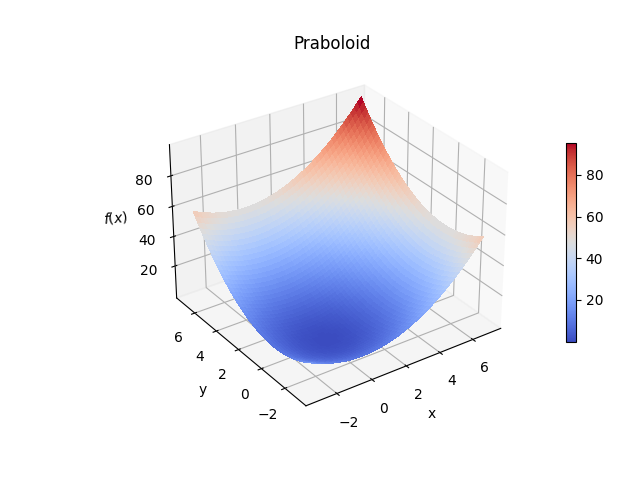
\includegraphics[scale=0.8]{Abbildungen/3D_Visualisationen/3D_visualization_paraboloid_2_-3_7_coolwarm.png}
		
		\caption{Paraboloid - Visualisierung in 3D}
		\label{fig:3D_Visualization_Paraboloid_2_-3_7}
	\end{figure}
	
	\subsubsection{Testfunktion - Easom} \label{subsubsec:Stetige_Testfunktionen:Testfunktion_-_Easom}
	
	Wie in \cite{molga2005test} beschrieben, ist die Easom-Testfunktion deswegen interessant, weil die Umgebung um das globale Minimum klein ist im Verhältnis zur Größe des gesamten Suchraumes. Der Suchraum ist das Quadrat \([-100, 100] \times [-100, 100]\) in der Abbildung~\ref{fig:3D_Visualization_Easom_Various_Intervals} links, während das Optimum im Quadrat \([1, 5] \times [1, 5]\) sich befindet, in der Abbildung~\ref{fig:3D_Visualization_Easom_Various_Intervals} rechts.
	
	\begin{figure}[H]
		
		\centering
		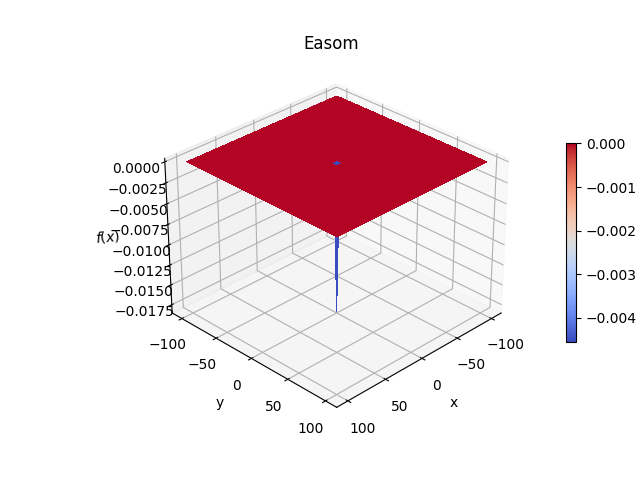
\includegraphics[width=.5\textwidth]{Abbildungen/3D_Visualisationen/3D_visualization_easom_2_-100_100_coolwarm.png}\hfill
		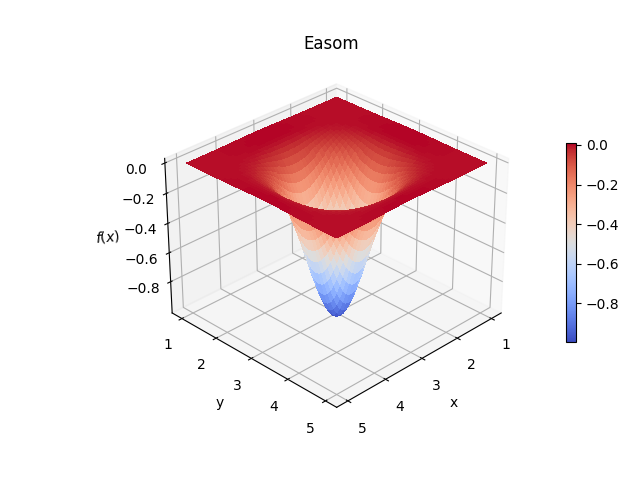
\includegraphics[width=.5\textwidth]{Abbildungen/3D_Visualisationen/3D_visualization_easom_2_1_5_coolwarm.png}
		
		\caption{Easom-Testfunktion: Vergleich zwischen gesamtem Suchraum (links) und Umgebung um das Optimum (rechts)}
		\label{fig:3D_Visualization_Easom_Various_Intervals}
		
	\end{figure}
	
	\subsubsection{Testfunktion - Griewangk} \label{subsubsec:Stetige_Testfunktionen:Testfunktion_-_Griewangk}
	
	Wie in \cite{molga2005test} beschrieben, ist die Griewangk-Testfunktion multimodal und hat damit viele lokale Optima, was die Suche nach dem globalen für Algorithmen erschwert. Ferner sind die lokalen Minima zwar gleich verteilt aber weit gestreut, was die Suche nach dem globalen Optima weiter verkompliziert. Die Griewangk-Testfunktion wurde auch deswegen gewählt, da, wie in Abbildung~\ref{fig:3D_Visualization_Griewangk_2_Various_Intervals} zu zusehen, sich das Aussehen der Funktion in Abhängigkeit vom Betrachtungsintervall ändert. Im Intervall \([-600,600]^n, n = 2\), was die 2-dimensionale Version des Initialisierungsintervall \([-600,600]^n, n = 10\) ist, welches für die Optimierung verwendet wird, muss der Algorithmus schnell konvergieren, um nicht viele Iterationen mit schlechten Werten zu verbrauchen. Im Intervall \([-10,10]^n, n = 2\), muss der Algorithmus Variabilität zeigen, um die große Menge an lokalen Minima zu meiden. Und schließlich im Intervall \([-4,4]^n, n = 2\), muss der Algorithmus eine aperiodische, zerklüftete Landschaft manövrieren, um das globale Optimum zu finden. Deswegen eignet sich die Griewangk-Testfunktion besonders gut, um das Können eines Algorithmus zu testen. 
	
	\begin{figure}[H]
		
		\centering
		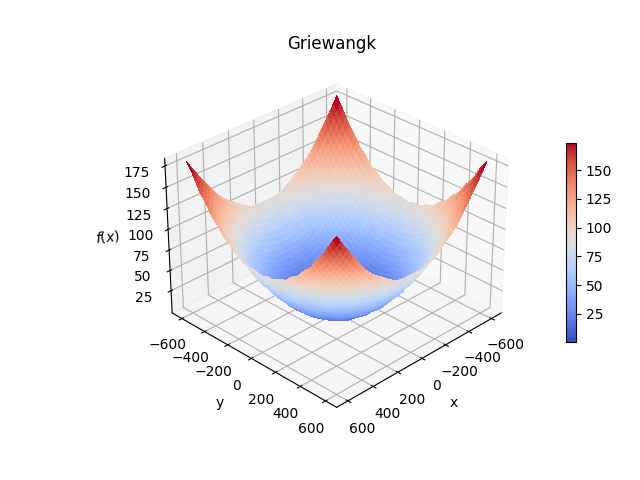
\includegraphics[width=.3\textwidth]{Abbildungen/3D_Visualisationen/3D_visualization_griewangk_2_-600_600_coolwarm.png}\hfill
		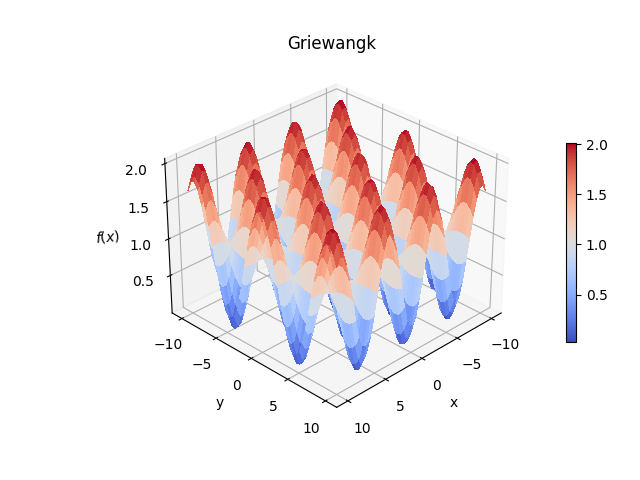
\includegraphics[width=.3\textwidth]{Abbildungen/3D_Visualisationen/3D_visualization_griewangk_2_-10_10_coolwarm.png}\hfill
		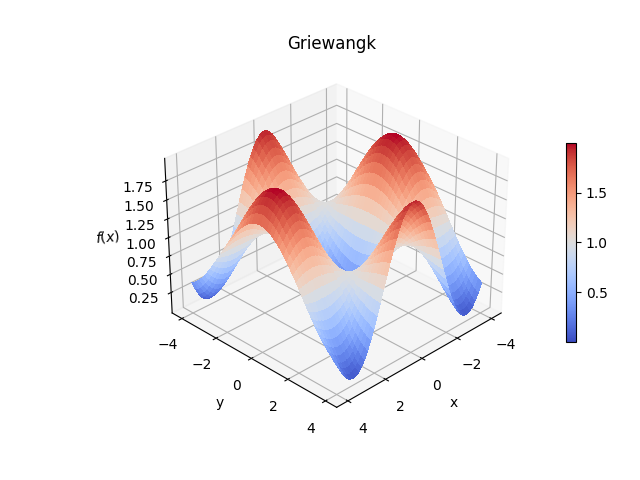
\includegraphics[width=.3\textwidth]{Abbildungen/3D_Visualisationen/3D_visualization_griewangk_2_-4_4_coolwarm.png}
		
		\caption{Verschiedene Auflösungen der Griewangk-Testfunktion}
		\label{fig:3D_Visualization_Griewangk_2_Various_Intervals}
		
	\end{figure}
	
	\subsubsection{Testfunktion - Rosenbrock} \label{subsubsec:Stetige_Testfunktionen:Testfunktion_-_Rosenbrock}
	
	Wie in \cite{molga2005test} beschrieben, zeichnet sich die Rosenbrock-Testfunktion dadurch aus, dass ihr Optimum in einem langen, engen Tal liegt. Es ist leicht das Tal zu finden aber es ist sehr schwer zum Optimum zu konvergieren. Die Rosenbrock-Testfunktion ist interessant, da sie sehr flach nahe dem Optimum ist und die Konvergenz langsam vorangeht. Die Rosenbrock-Testfunktion wurde auch aus dem Grund gewählt, weil in meiner Bachelorarbeit~\cite{FCM_2019}, unter den Testfunktionen zum Vergleich mit Algorithmen, die probabilistisches Lernen einsetzen, den Testfunktionen aus Tabelle~\ref{subsec:Stetige_Testfunktionen:tab:Prob_Lernen}, es die einzige Testfunktion war, bei welcher der \acl{acorvs} nicht der beste Algorithmus oder zumindest sehr gut. Bei dieser Testfunktion konnte ACO\(_\mathbb{R}\)-VS das Optimum nicht finden. Deswegen ist diese Testfunktion besonders interessant, um die Variationen von ACO\(_\mathbb{R}\)-VS zu testen.
	
	\begin{figure}[H]
		\centering
		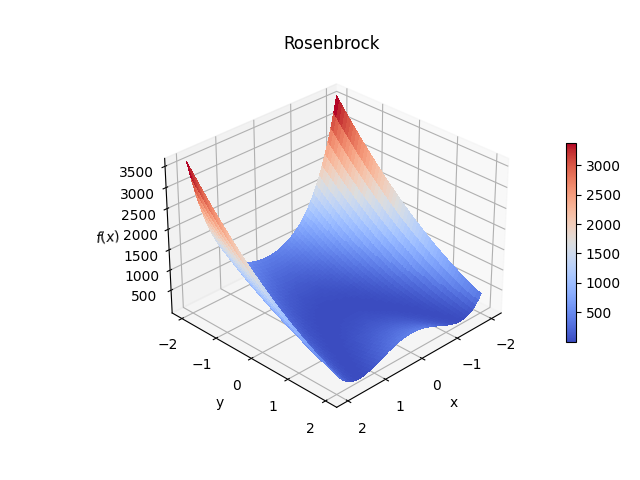
\includegraphics[scale=0.8]{Abbildungen/3D_Visualisationen/3D_visualization_rosenbrock_2_-2_2_coolwarm.png}
		
		\caption{Rosenbrock - Visualisierung in 3D}
		\label{fig:3D_Visualization_Rosenbrock_2-2_2}
	\end{figure}
	
	\subsubsection{Testfunktion - Hartmann} \label{subsubsec:Stetige_Testfunktionen:Testfunktion_-_Hartmann}
	
	Die Familie der Hartmann-Testfunktionen ist eine der beiden Familien der komplexen Testfunktionen, die in dieser Arbeit betrachtet werden. Diese Familie zeichnet sich dadurch aus, dass sie die leichtere der beiden komplexen Testfunktionfamilien ist. Sie ist multimodal mit 4 lokalen Minima im Fall von Hartmann(3,4), und respektive 6 lokalen Minima im Fall von Hartmann(6,4).
	
	\begin{figure}[H]
		
		\centering
		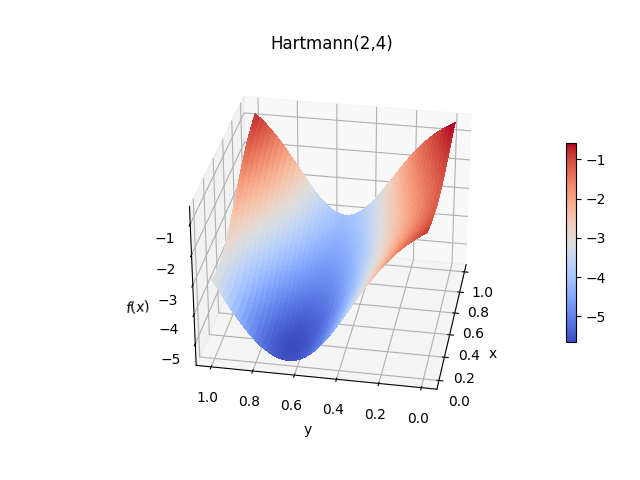
\includegraphics[width=.5\textwidth]{Abbildungen/3D_Visualisationen/3D_visualization_hartmann_not_3_2_4_0_1_coolwarm.png}\hfill
		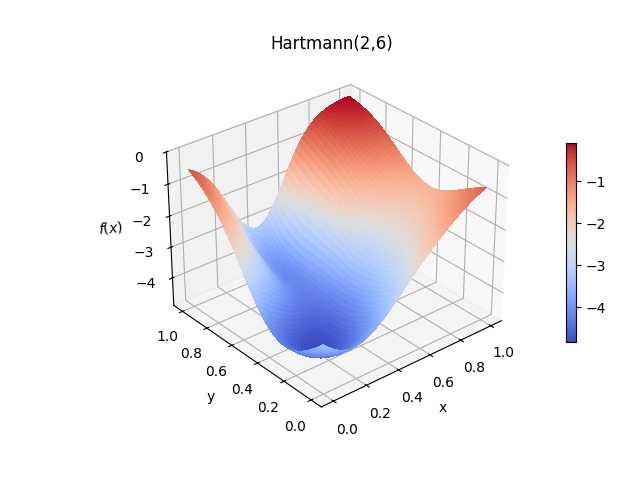
\includegraphics[width=.5\textwidth]{Abbildungen/3D_Visualisationen/3D_visualization_hartmann_not_6_2_4_0_1_coolwarm.png}
		
		\caption{Hartmann-Testfunktionen: Hartmann(2,4) (links) und Hartmann(2,6) (rechts)}
		\label{fig:3D_Visualization_Hartmann_Various_Dimensions}
		
	\end{figure}
	
	\subsubsection{Testfunktion - Shekel} \label{subsubsec:Stetige_Testfunktionen:Testfunktion_-_Shekel}
	
	Die Familie der Shekel-Testfunktionen ist die schwerere der beiden komplexen Testfunktionfamilien, die in dieser Arbeit betrachtet werden. Sie ist multimodal und hat 5 lokale Minima im Fall von Shekel(4,5), 7 lokale Minima im Fall von Shekel(4,7) und respektive 10 lokale Minima im Fall von Shekel(4,10).
	
	\begin{figure}[H]
		
		\centering
		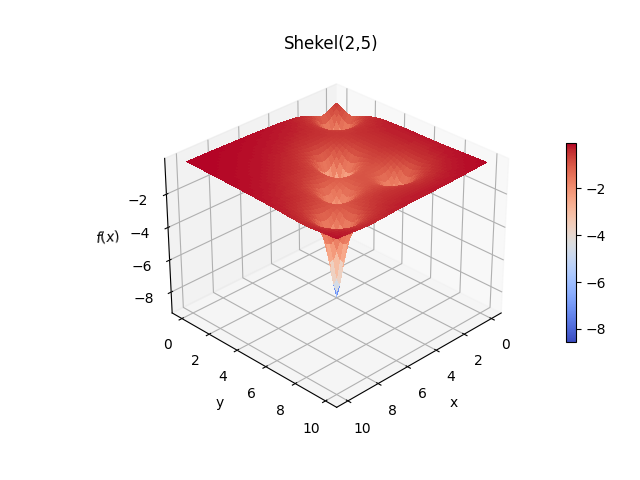
\includegraphics[width=.3\textwidth]{Abbildungen/3D_Visualisationen/3D_visualization_shekel_2_5_-0_10_coolwarm.png}\hfill
		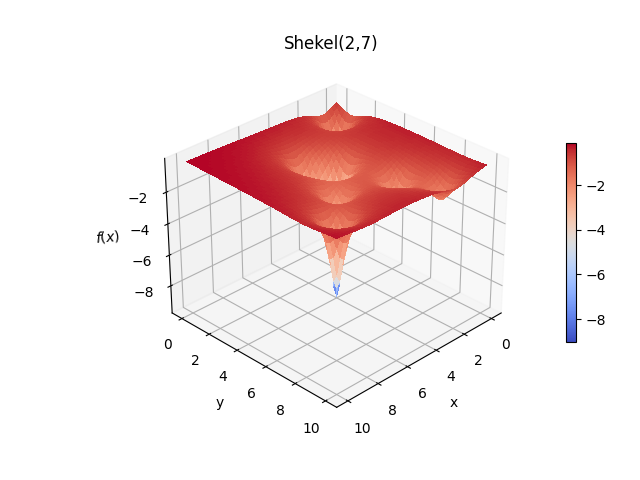
\includegraphics[width=.3\textwidth]{Abbildungen/3D_Visualisationen/3D_visualization_shekel_2_7_-0_10_coolwarm.png}
		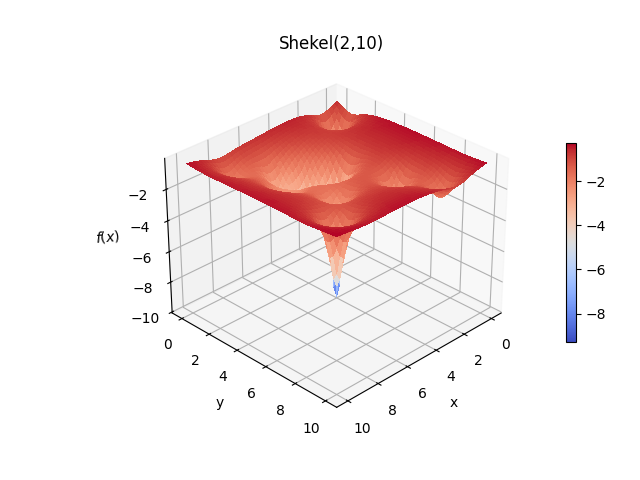
\includegraphics[width=.3\textwidth]{Abbildungen/3D_Visualisationen/3D_visualization_shekel_2_10_-0_10_coolwarm.png}
		
		\caption{Shekel-Testfunktionen: Shekel(2,5) (links), Shekel(2,7) (mittig) und Shekel(2,10) (rechts)}
		\label{fig:3D_Visualization_Shekel_Various_Number_Of_Lokal_Minima}
		
	\end{figure}
	
	\subsection{Testfunktionen mit gemischten Variablen} \label{subsec:Mixed_Variable}
	
	\subsubsection{Konstruierte Testfunktionen} \label{subsubsec:Konstruierte_Probleme}
	
	Neue Testfunktionen mit gemischten Variablen wurden erzeugt, indem die stetigen Testfunktionen aus Tabelle~\ref{subsec:Stetige_Testfunktionen:tab:Prob_Lernen}, außer \glqq Rosenbrock\grqq, genommen wurden und ein Teil ihrer Dimensionen zu diskreten Dimensionen transformiert wurde. Im JSON-Format wird dies wie im Code-Snipped~\ref{subsubsec:Testfunktionen:Konstruierte_Testfunktionen:JSON:Paraboloid5Dim11MV} angezeigt.
	
	\begin{lstlisting}[language=json, caption=Paraboloid 5 Dim gemischte Variablen, label=subsubsec:Testfunktionen:Konstruierte_Testfunktionen:JSON:Paraboloid5Dim11MV]
{
"name": "Paraboloid_5_11_MV",
"comment": "artificial mixed_variable problem",
"type": "mixed variable problems",
"continuous_dimension": 3,
"discrete_dimension": 2,
"dimension": 5,
"optimum_argument": [[0.0], [0.0], [0.0], [0.0], [0.0]],
"optimum": [0.0],

"variable_boundaries": {
	"natural_numbers": [],
	"discrete": [[-3, 7]],
	"continuous": [[-3, 7]],
	"ordinal": [],
	"categorical": []
},

"discrete_values": [-3.0, -2.0, -1.0, 0.0, 1.0,
2.0, 3.0, 4.0 ,5.0, 6.0,
7.0],

"magnitudes_of_categorical_variables": []
}
	\end{lstlisting}
	
	Es wurden die Testfunktionen \glqq Cigar\grqq, \glqq Ellipsoid\grqq, \glqq Paraboloid\grqq{} und \glqq Tablet\grqq{} aus Tabelle~\ref{subsec:Stetige_Testfunktionen:tab:Prob_Lernen} gewählt, da sie sowohl für verschiedene Dimensionen, diskret und stetig, definiert werden konnten, als auch wo die Algorithmen, bis auf wenige Ausnahmen, konvergierten. Im Vergleich werden Kombinationen aus verschiedenen Anzahlen an Dimensionen und verschiedenen Anzahlen an diskreten Punkten untersucht. Jede der Testfunktionen wird mit den Dimensionen \(n = \{2, 5, 10\}\) und mit der Anzahl an diskreten Punkten \(m \in \{11, 21, 51\}\) getestet. Dabei wird jede der Dimensionen mit allen Anzahlen an diskreten Punkten getestet, also ergeben sich \((2,11), (2,21), (2,51), \dots, (10, 11), (10,21), (10,51)\) als Kombinationen pro Testfunktion. Zusätzlich wird jede Funktion mit den beiden Neustartstrategien \(fixed = n, n \in \mathbb{N}\) und \(adaptive\) getestet, wobei \(n = 0\) gesetzt wurde. Damit ergeben sich 72 konstruierte Testfunktionen, wie in den Tabellen \ref{subsec:Vergleich_Von_ACO_R_ACO_R_Very_Simple_Und_Iterationen:tab:Vergleich_Probabilistisches_Lernen_Funktionen_Mit_Gemischten_Variablen_Teil_1} und \ref{subsec:Vergleich_Von_ACO_R_ACO_R_Very_Simple_Und_Iterationen:tab:Vergleich_Probabilistisches_Lernen_Funktionen_Mit_Gemischten_Variablen_Teil_2} zu sehen. Testfunktionen, deren Anzahl an Dimension \(5\) ist, haben als Anzahl an stetigen Dimensionen \(3\) und als Anzahl an diskreten Dimensionen \(2\), wie im Code-Snipped~\ref{subsubsec:Testfunktionen:Konstruierte_Testfunktionen:JSON:Paraboloid5Dim11MV} zu sehen. Die Dimension von Testfunktionen, deren Dimension gerade ist, also \(2\) oder \(10\), setzt sich zusammen aus Hälfte diskreter Dimensionen und aus Hälfte stetiger Dimensionen. Das Abbruchkriterium für alle die so konstruierten Testfunktionen ist das selbe, wie für Testfunktionen aus Tabelle~\ref{subsec:Stetige_Testfunktionen:tab:Prob_Lernen}, nämlich \(|f - f^*| < \varepsilon, \, \varepsilon = 10^{-10}\). Es wurde das selbe Abbruchkriterium verwendet, um Vergleichbarkeit zu ermöglichen.
	
	\subsubsection{Coil Spring Design Problem (CSD)} \label{subsubsec:Coil_Spring_Design_Problem}
	
	Das Coil Spring Design Problem (CSD) kann auf verschiedene Arten definiert werden, wie in \cite{sandgren1990nonlinear}, \cite{guo2004swarm} oder später, aufbauend auf \cite{sandgren1990nonlinear}, in \cite{ACO_2013}. In dieser Arbeit wird die Definition aus \cite{ACO_2013} verwendet. Im CSD Problem, wie es in \cite{ACO_2013} definiert wird, wird so nach dem Außendurchmesser \(D\), dem Drahtdurchmesser \(d\) und der Windungszahl \(N\) einer Schraubenfeder (Coil Spring), wie sie in Abbildung~\ref{subsubsec:Testfunktionen:CSD:fig:CSD_schematical} skizzenhaft dargestellt ist, gesucht, dass der Materialbedarf für die Schraubenfeder minimiert wird, während gleichzeitig die Nebenbedingungen (Constrains) erfüllt werden.\\
	
	\begin{figure}[H]
		\centering
		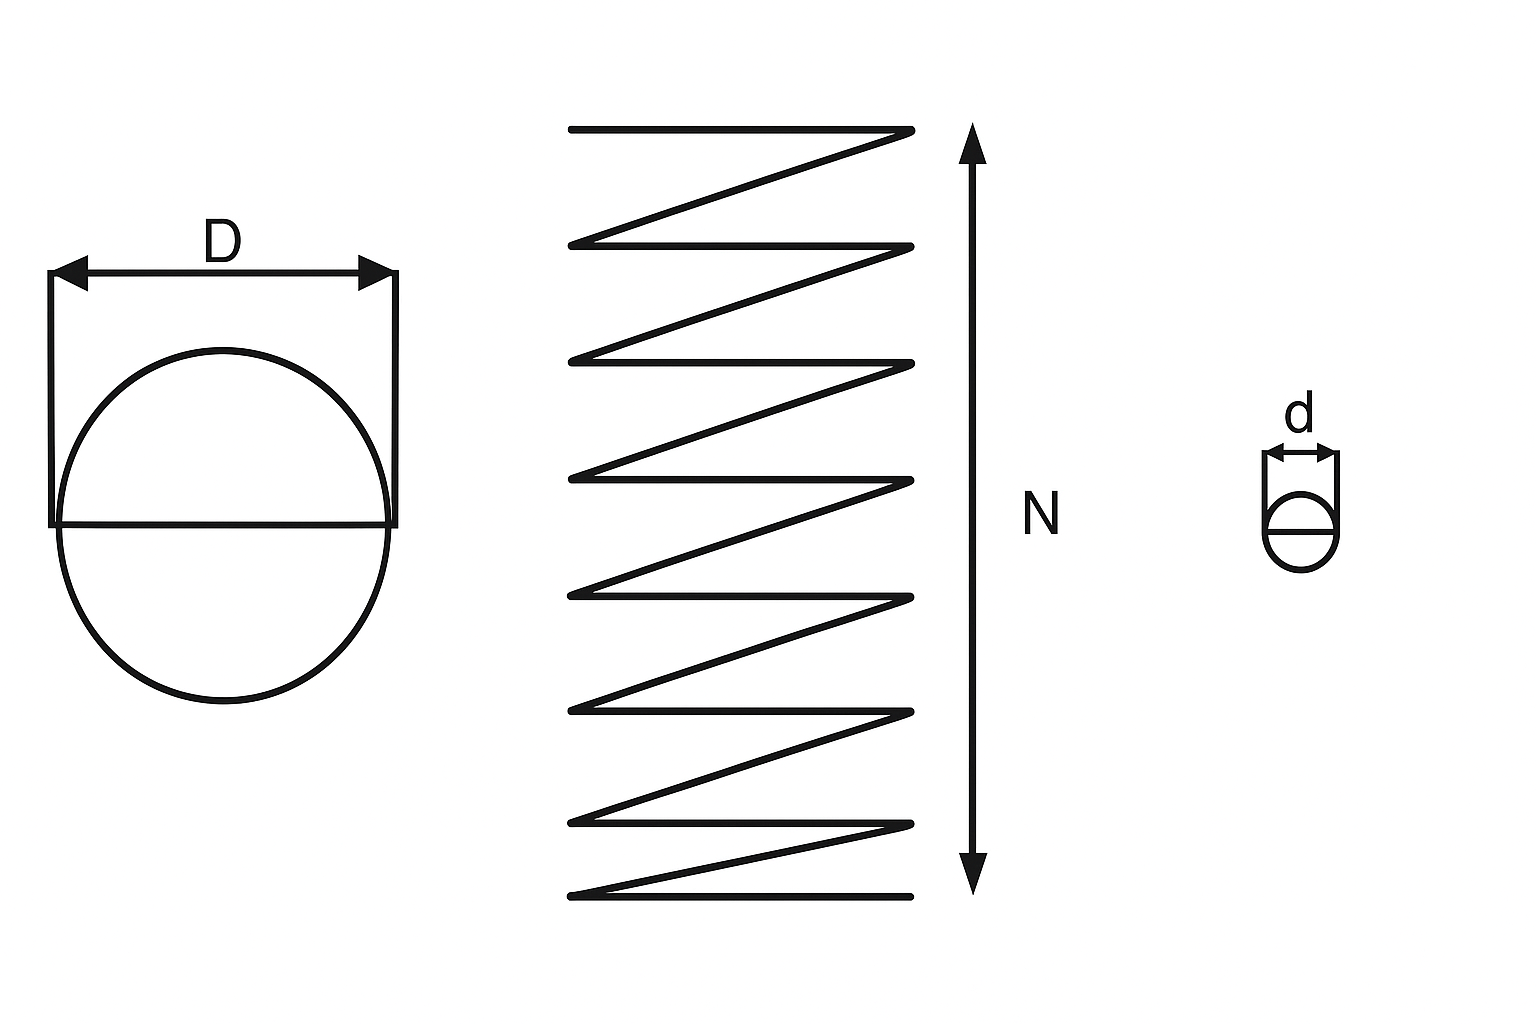
\includegraphics[scale=0.2]{Abbildungen/Coil_Spring_Design_-_Dateien/CSD_schematical.png}
		\caption{Skizze einer Schraubenfeder mit Federdurchmesser (links), Windungszahl (mitte) und Drahtdurchmesser (rechts)¨; das Bild wurde von mir mit einem Zeichenprogramm erstellt und dann mit ChatGPT verbessert}
		\label{subsubsec:Testfunktionen:CSD:fig:CSD_schematical}
	\end{figure}
	
	\noindent Da in \textit{Sandgren}~\cite{sandgren1990nonlinear} das CSD Problem initial in imperialen Maßeinheiten definiert wurde, verwendeten alle Folgestudien, wie \cite{deb1998flexible}, \cite{Lampinen1999MIXEDIO}, \cite{guo2004swarm}, \cite{gong2022novel}, \cite{kannan1994augmented} oder \cite{ACO_2013}, ebenfalls imperiale Maßeinheiten, um die Ergebnisse vergleichen zu können. Deswegen werden auch in dieser Arbeit imperiale Maßeinheiten verwendet.\\
	
	\noindent Das Problem zählt zu Problemen mit gemischten Variablen, da \(D\) eine stetige und \(d\) eine ordinale Variable ist. \(N\) ist eine Variable, die nur natürliche Zahlen als Werte annehmen kann.\\
	
	\noindent Mögliche Werte, die der Drahtdurchmesser \(d\) annehmen kann, sind in der Tabelle~\ref{table:d_values} aufgelistet.
	
	\begin{table}[H]
		
		\fontsize{10pt}{12pt}
		
		\caption{Standarddrahtdurchmesser für die Schraubenfeder angegeben in Zoll (inch)}
		
		\label{table:d_values}
		
		\begin{center}
		
			\begin{tabular}{c c c c c c}
				
				\hline
				
				0.0090 & 0.0095 & 0.0104 & 0.0118 & 0.0128 & 0.0132\\
				
				0.0140 & 0.0150 & 0.0162 & 0.0173 & 0.0180 & 0.0200\\
				
				0.0140 & 0.0150 & 0.0162 & 0.0173 & 0.0180 & 0.0200\\
				
				0.0470 & 0.0540 & 0.0630 & 0.0720 & 0.0800 & 0.0920\\
				
				0.1050 & 0.1200 & 0.1350 & 0.1480 & 0.1620 & 0.1770\\
				
				0.1920 & 0.2070 & 0.2250 & 0.2440 & 0.2630 & 0.2830\\
				
				0.3070 & 0.3310 & 0.3620 & 0.3940 & 0.4375 & 0.5000\\
				
				\hline
				
			\end{tabular}
		
		\end{center}
		
	\end{table}
	
	\noindent Weiter werden in \cite{ACO_2013} Intervallgrenzen definiert, die in der Tabelle~\ref{table:int_restrict} aufgeführt werden. Es fällt auf, dass durch die Definition der Intervallgrenze \(d_{min}\) = 0.2 Zoll (inch), 31 der 42 möglichen Werte, welche die diskrete Variable \(d\) annehmen kann, wegfallen, aber dies ist so in \textit{Sandgren}~\cite{sandgren1990nonlinear} angegeben und die Folgequellen \cite{deb1998flexible}, \cite{Lampinen1999MIXEDIO}, \cite{guo2004swarm}, \cite{gong2022novel}, \cite{kannan1994augmented} und \cite{ACO_2013} verwenden die Intervallgrenze direkt oder verweisen auf \textit{Sandgren}~\cite{sandgren1990nonlinear}. Keine der Quellen gibt eine Begründung an. Um Vergleichbarkeit zu garantieren, wird \(d_{min}\) = 0.2 beibehalten.
	
	\begin{table}[H]
		
		\fontsize{10pt}{12pt}
		
		\caption{Intervallgrenzen}
		
		\label{table:int_restrict}
		
		\begin{center}
			
			\begin{tabular}{l l}
				
				\hline
				
				maximale Arbeitsbelastung & \(F_{max}\) = 1000.0 Pfund (lb)\\
				
				zulässige maximale Scherspannung & \(S\) = 189000.0 Pfund pro Quadratzoll (psi)\\
				
				maximale freie Länge & \(l_{max}\) = 14.0 Zoll (inch)\\
				
				Mindestdrahtdurchmesser & \(d_{min}\) = 0.2 Zoll (inch)\\
				
				maximaler Außendurchmesser & \(D_{max}\) = 3.0 Zoll (inch)\\
				
				der Feder & \\
				
				Vorspannkompressionskraft & \(F_p\) = 300.0 Pfund (lb)\\
				
				zulässige maximale Durchbiegung & \(\sigma_{pm}\) = 6.0 Zoll (in)\\
				
				unter Vorspannung & \\
				
				Auslenkung von der Vorlastposition & \(\sigma_{w}\) = 1.25 Zoll (in)\\
				
				zur Maximallastposition & \\
				
				Schubmodul des Materials & \(G\) = 11.5 \(\cdot\) 10\(^6\)\\
				
				\hline
				
			\end{tabular}
			
		\end{center}
		
	\end{table}
	
	\noindent Die Nebenbedingen umfassen primäre und sekundäre Variablen. Die primären Variablen sind \(D\), \(d\) und \(N\). Die sekundären Variablen sind \(C_f\), \(K\), \(\sigma_p\) und \(l_f\). Die sekundären Variablen ergeben sich aus den primären Variablen und den Intervallgrenzen und werden in den Gleichungen~\ref{eq:C_f}~bis~\ref{eq:l_f} definiert. Die Definitionsbereiche der primären Variablen können der Tabelle~\ref{table:prim_var_domain} entnommen werden.\\
	
	\begin{table}[H]
		
		\fontsize{10pt}{12pt}
		
		\caption{Definitionsbereiche}
		
		\label{table:prim_var_domain}
		
		\begin{center}
			
			\begin{tabular}{l l}
				
				\hline
				
				D & \{3d, 3.0\}\\
				
				d & \{d\(_{min}\), 0.5000\}\\
				
				N & \{1, 70\}\\
				
				\hline
				
			\end{tabular}
			
		\end{center}
		
	\end{table}
	
	\begin{equation} \label{eq:C_f}
		C_f = \frac{4 \frac{D}{d} - 1}{4 \frac{D}{d} - 4} + \frac{0.615d}{D}
	\end{equation}
	
	\begin{equation} \label{eq:K}
		K = \frac{G d^4}{8 N D^3}
	\end{equation}
	
	\begin{equation} \label{eq:sigma_p}
		\sigma_p = \frac{F_p}{K}
	\end{equation}
	
	\begin{equation} \label{eq:l_f}
		l_f = \frac{F_{max}}{K} + 1.05 (N + 2) d
	\end{equation}\\
	
	\noindent Ferner unterliegen die Variablen im CSD 8 Constrains \(c_i, \, i \in \{1, \dots, 8\}\). Diese sind in Tabelle~\ref{table:variable_restrict} dargelegt.
	
	\begin{table}[H]
		
		\fontsize{12pt}{12pt}
		
		\caption{Constrains}
		
		\label{table:variable_restrict}
		
		\begin{center}
			
			\def\arraystretch{1.5}
			
			\begin{tabular}{| l | c |}
				
				\hline
				
				1 & \(c_1\) = \(\frac{8 C_f F_{max} D}{\pi d^3} - S \leq 0\)\\
				
				\hline
				
				2 & \(c_2\) = \(l_f - l_{max} \leq 0\)\\
				
				\hline
				
				3 & \(c_3\) = \(d_{min} - d \leq 0\)\\
				
				\hline
				
				4 & \(c_4\) = \(D - D_{max} \leq 0\)\\
				
				\hline
				
				5 & \(c_5\) = \(3.0 - \frac{D}{d}\)\\
				
				\hline
				
				6 & \(c_6\) = \(\sigma_p - \sigma_{pm} \leq 0\)\\
				
				\hline
				
				7 & \(c_7\) = \(\sigma_p + \frac{F_{max} - F_p}{K} + 1.05 (N + 2) d - l_f \leq 0\)\\
				
				\hline
				
				8 & \(c_8\) = \(\sigma_{w} - \frac{F_{max} - F_p}{K} \leq 0\)\\
				
				\hline
				
			\end{tabular}
			
		\end{center}
		
	\end{table}
	
	\noindent Der Materialbedarf und damit die Zielfunktion wird mit Hilfe der Formel~\ref{subsubsec:Testfunktionen:CSD:eq:CSD_material} berechnet.
	
	\begin{equation} \label{subsubsec:Testfunktionen:CSD:eq:CSD_material}
		f(N, D, d) = \frac{\pi^2 D d^2 (N + 2)}{4}
	\end{equation}

	Schließlich wird das Abbruchkriterium als \(|f - f^*| < |\varepsilon_1 f| + \varepsilon_2, \, \varepsilon_1 = \varepsilon_2 = 10^{-6}\) gewählt. Dieses Abbruchkriterium wird gewählt, da davon ausgegangen wird, dass in \textit{Socha}~\cite{socha2009ant} das selbe Kriterium benutzt wurde und es eine Erweiterung des Abbruchkriteriums \(|f - f^*| < |\varepsilon_1 f| + \varepsilon_2, \, \varepsilon_1 = \varepsilon_2 = 10^{-4}\) ist, welches für den Großteil der stetigen Testfunktionen in dieser Arbeit verwendet wurde. Leider ist in \textit{Socha}~\cite{socha2009ant} das Abbruchkriterium für das \ac{csd} nicht angegeben.
	
	\paragraph{Vollständiger Raum als Initialisierungsintervall}\mbox{}\\
	\newline
	\noindent Wie bereits im Abschnitt~\ref{sec:Testfunktionen} beschrieben, hat das Initialisierungsintervall großen Einfluss auf den Erfolg %die Güte?
	des Algorithmus. So können für das CSD Anfangslösungen aus dem gesamten Raum \(\{3 \cdot d_{min}, 3.0\} \times \{d_{min}, 0.5000\} \times \{1, 70\}\) oder dem gefilterten Raum gezogen werden.\hfill\newline
	
	Nimmt man den gesamten Raum zum ziehen der Initiallösungen, so ändert sich die Zielfunktion von der Formel~\ref{subsubsec:Testfunktionen:CSD:eq:CSD_material} zu der Formel~\ref{subsubsec:Testfunktionen:CSD:eq:CSD_penalty}, wie in \cite{ACO_2013} definiert.
	
	\begin{equation} \label{subsubsec:Testfunktionen:CSD:eq:CSD_penalty}
		\hat{f} = f \prod_{i = 1}^{8} \hat{c_i}^3 
	\end{equation}
	
	Dabei werden die \(\hat{c_i}\)'s in der Formel~\ref{subsubsec:Testfunktionen:CSD:eq:CSD_c_i} definiert.
	
	\begin{equation} \label{subsubsec:Testfunktionen:CSD:eq:CSD_c_i}
		\hat{c_i} =
		\begin{cases}
			\begin{aligned}
				& 1 + w_i c_i, &&\text{wenn } c_i > 0\\
				& 1, &&\text{sonst}
			\end{aligned}
		\end{cases}
	\end{equation}
	
	Die Gewichte \(w_i, \, i \in \{1, \dots, 8\}\) wurden aus \cite{ACO_2013} entnommen und befinden sich in der Tabelle~\ref{table:CSD_penalty_weights}.
	
	\begin{table}[H]
		
		\fontsize{12pt}{12pt}
		
		\caption{Gewichte}
		
		\label{table:CSD_penalty_weights}
		
		\begin{center}
			
			\def\arraystretch{1.5}
			
			\begin{tabular}{| l | c |}
				
				\hline
				
				1 & \(w_1 = \) 10\(^{-5}\)\\
				
				\hline
				
				2 & \(w_2 =\) 1\\
				
				\hline
				
				3 & \(w_3 =\) 10\(^2\)\\
				
				\hline
				
				4 & \(w_4 =\) 1\\
				
				\hline
				
				5 & \(w_5 =\) 10\(^2\)\\
				
				\hline
				
				6 & \(w_6 =\) 1\\
				
				\hline
				
				7 & \(w_7 =\) 10\(^2\)\\
				
				\hline
				
				8 & \(w_8 =\) 10\(^2\)\\
				
				\hline
				
			\end{tabular}
			
		\end{center}
		
	\end{table}
	
	\paragraph{Gefilterter Raum als Initialisierungsintervall}\mbox{}\\
	\newline
	
	\noindent Benutzt man den gefilterten Raum, kann die Formel~\ref{subsubsec:Testfunktionen:CSD:eq:CSD_material} ohne Veränderungen beibehalten werden. Abbildung~\ref{subsubsec:Testfunktionen:CSD:fig:3D_plot:CSD:filtered_and_unfiltered_search_spaces} zeigt, wie stark sich der Initialisierungsraum verkleinert und damit die Lösungssuche erleichtert wird, wenn der Initialisierungsraum vor dem Ausführen des Algorithmus nach gültigen Lösungen gefiltert wird. Wie zu sehen verkleinert sich der Initialisierungsraum um mehr als das Achtfache. Alle Abbildungen in diesem Abschnitt wurden von mir mit den Python-Bibliotheken \glqq numpy\grqq{} und \glqq matplotlib\grqq{} erstellt.
	
	\begin{figure}[H]
		\centering
		\subfloat[][gefilterter Raum]{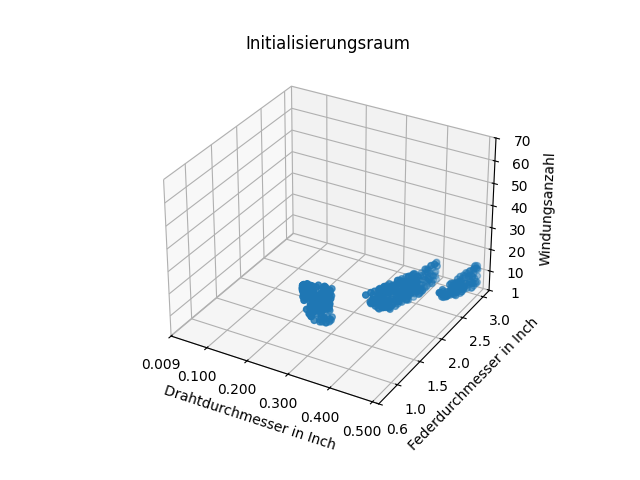
\includegraphics[width=0.4\linewidth]{Abbildungen/3D_Visualisationen/3D_visualization_CSD_filtered_space.png}}
		\qquad
		\subfloat[][ungefilterter Raum]{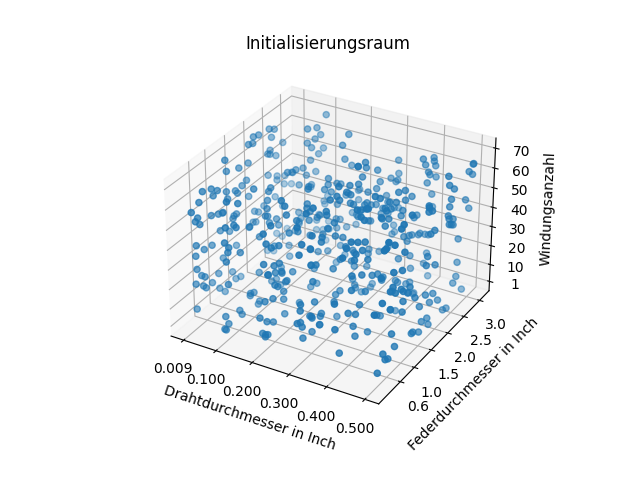
\includegraphics[width=0.4\linewidth]{Abbildungen/3D_Visualisationen/3D_visualization_CSD_unfiltered_space.png}}
		\caption{gefilterter und ungefilterter Suchraum für das CSD-Problem}
		\label{subsubsec:Testfunktionen:CSD:fig:3D_plot:CSD:filtered_and_unfiltered_search_spaces}
	\end{figure}
	
	\noindent Um zu zeigen, wie stark der Initialisierungsraum sich verkleinert, werden die beiden Initialisierungsräume, wie in Abbildung~\ref{subsubsec:Testfunktionen:CSD:fig:3D_plot:CSD:filtered_and_unfiltered_search_spaces_combined}, übereinander gelegt.
	
	\begin{figure}[H]
		\centering
		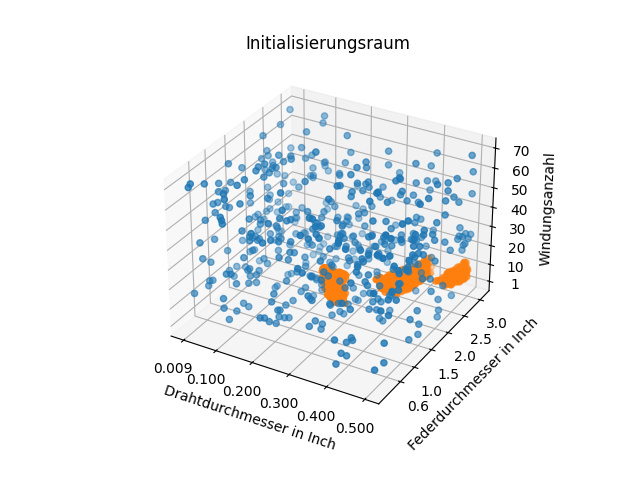
\includegraphics[scale=0.5]{Abbildungen/3D_Visualisationen/3D_visualization_CSD_unfiltered_and_filtered_space.png}
		\caption{gefilterter Raum (orange) und ungefilterter Raum (blau)}
		\label{subsubsec:Testfunktionen:CSD:fig:3D_plot:CSD:filtered_and_unfiltered_search_spaces_combined}
	\end{figure}

	\paragraph{Resultierende Testkombinationen für das \ac{csd}}\mbox{}\\
	
	Wie dargelegt, kann der Suchraum genommen werden ohne Filterung und mit Filterung. Zusätzlich kann die Zielfunktion exakt formuliert werden, wie in Gleichung~\ref{subsubsec:Testfunktionen:CSD:eq:CSD_material} und mit Straftermen, wie in Gleichung~\ref{subsubsec:Testfunktionen:CSD:eq:CSD_penalty}. Schließlich werden noch zwei Neustartstrategien, \(fixed = 0\) und \(adaptvie\), betrachtet. Damit ergeben sich 8 Kombinationen die getestet werden, wie in den Tabellen \ref{subsubsec:Vergleich_Von_ACO_R_ACO_R_Very_Simple_Und_Iterationen:tab:Vergleich_CSD_fixed} und \ref{subsubsec:Vergleich_Von_ACO_R_ACO_R_Very_Simple_Und_Iterationen:tab:Vergleich_CSD_adaptive} zu sehen.

	\section{Vergleich von ACO\(_{\mathbb{R}}\), ACO\(_\text{MV}\) und den Varianten von \acl{acorvsmv}} \label{sec:Vergleich_Von_ACO_R_ACO_R_Very_Simple_Und_Den_Iterationen_Von_ACO_R_Very_Simple}
	
	Alle Varianten von \ac{acorvsmv} können mit gemischten Variablen umgehen. Aus Platzgründen wurde in den Tabellen das \glqq -MV\grqq{} weggelassen.
	
	\subsection{Vergleich bzgl. stetiger Testfunktionen} \label{subsec:Vergleich_Algorithmen:Vergleich_Auf_Stetigen_Testfunktionen}
	
	Da in \textit{Socha}~\cite{socha2009ant} ACO\(_\text{MV}\) erst dann eingeführt wird, wenn Testfunktionen mit gemischten Variablen eingeführt werden, kann in diesem Abschnitt nur mit ACO\(_\mathbb{R}\) aus \cite{socha2009ant} verglichen werden. Ferner werden in diesem Abschnitt nur Minimierungtestfunktionen betrachtet, also Testfunktionen, bei denen das globale Minimum gesucht ist, da die Varianten von \ac{acorvsmv} nicht mit Testfunktionen umgehen können, bei denen das Optimum außerhalb des Definitionsbereichs liegt, was bei den Maximierungstestfunktionen \glqq Diagonale Plane\grqq{} und \glqq Pane\grqq{} der Fall ist. Damit entfallen die beiden Maximierungstestfunktionen \glqq Diagonale Plane\grqq{} und \glqq Plane\grqq. Alle Testfunktionen wurden 50 mal durchlaufen.\hfill\newline
	
	Wie in den Tabellen \ref{subsec:Vergleich_Von_ACO_R_ACO_R_Very_Simple_Und_Iterationen:tab:Vergleich_Probabilistisches_Lernen_Teil_1} und \ref{subsec:Vergleich_Von_ACO_R_ACO_R_Very_Simple_Und_Iterationen:tab:Vergleich_Probabilistisches_Lernen_Teil_2} zu sehen, ist \ac{acorvs} des beste Algorithmus in 3 von 5 Testfunktionen und sehr gut in Einer. Nur bei der Testfunktion \glqq Rosenbrock\grqq{} konvergiert \ac{acorvs} nicht. Die Leistungen von \ac{acorvsmv} mit NSS-f0 sind dagegen schlechter. Die Varianten von \ac{acorvsmv} mit NSS-adapt sind nicht aufgeführt, da keine der Varianten von \ac{acorvsmv} mit NSS-adapt bei keiner der Testfunktionen aus den Tabellen \ref{subsec:Vergleich_Von_ACO_R_ACO_R_Very_Simple_Und_Iterationen:tab:Vergleich_Probabilistisches_Lernen_Teil_1} und \ref{subsec:Vergleich_Von_ACO_R_ACO_R_Very_Simple_Und_Iterationen:tab:Vergleich_Probabilistisches_Lernen_Teil_2} konvergierte. Positiv fallen zudem die Algorithmen ACO\(_\mathbb{R}\) und CMA-ES auf, da ihre relative Anzahl an Funktionsauswertungen nur wenig schlechter sind, als der Bestwert, außer bei der Testfunktion \glqq Ellipsoid\grqq.\hfill\newline
	
	Es folgt, dass unter den Algorithmen, die probabilistisches Lernen einsetzten, \ac{acorvs} der bessere Algorithmus ist, knapp gefolgt von ACO\(_\mathbb{R}\) und CMA-ES. Auf der anderen Seite, gemessen daran, dass die Varianten von \ac{acorvsmv}, unabhängig der Neustartstrategie, sowohl komplexer als \ac{acorvs} sind, als auch schlechter, sofern sie konvergieren, schlussfolgern wir, dass die Erweiterung von \ac{acorvs} zu den Varianten von \ac{acorvsmv}, bei Testfunktionen, welche zum Vergleich für Algorithmen, die probabilistisches Lernen einsetzten, genommen werden, keinen Mehrwert brachte.
	
	\begin{table}[H]
		
		\caption{Vergleich der Ergebnisse zwischen Algorithmen, die probabilistisches Lernen einsetzen, basierend auf \textit{Socha und Dorigo}~\cite{socha2008ant}, und damit auf \textit{Kern et al., 2004}~\cite{kern2004learning}}
		
		\label{subsec:Vergleich_Von_ACO_R_ACO_R_Very_Simple_Und_Iterationen:tab:Vergleich_Probabilistisches_Lernen_Teil_1}
		
		\scriptsize
		
		\begin{tabularx}{\linewidth}{l l l l l l l}
			
			\toprule
			
			Testfunktion & (1 + 1)ES & CSA-ES & CMA-ES & IDEA & MBOA & Bestwert\\
			
			\midrule
			
			Cigar & 1149.9 (2342400) & 1508.1 (3072000) & 1.9 (3840) & 8.7 (17664) & 22.6 (46080) & \textbf{1.0} (2037)\\
			
			Ellipsoid & 456.1 (293700) & 760.1 (489500) & 6.9 (4450) & 11.1 (7120) & 96.7 (62300) & \textbf{1.0} (644)\\
			
			Paraboloid & \textbf{1.0} (1370) & 1.6 (2192) & 1.3 (1781) & 5.0 (6850) & 48 (65760)  & \textbf{1.0} (1370)\\
			
			Rosenbrock & *51 (366690) & 180 (1294200) & \textbf{1.0} (7190) & *210 (1509900) & *1100 (7909000) & \textbf{1.0} (7190)\\
			
			Tablet & 67.4 (118082) & 95.3 (166855) & 2.5 (4364) & 4.3 (7445) & 35.2 (61608) & \textbf{1.0} (1751)\\
			
			\bottomrule
			
		\end{tabularx}
		
		\smallskip
		
		Dargestellt ist zuerst die relative Anzahl an Funktionsauswertungen und in Klammern danach die absolute. Bei Ergebnissen, wo ein * steht, wurde die erforderliche Genauigkeit nicht bei jedem Durchlauf des Algorithmus erreicht und dort wo \(\infty\) steht, wurde die Genauigkeit bei keinem Durchlauf des Algorithmus erreicht.\hfill\newline
		
	\end{table}
	
	\begin{table}[H]
		
		\caption{Vergleich der Ergebnisse zwischen ACO\(_{\mathbb{R}}\), ACO\(_{\mathbb{R}}\)-very-simple und den Varianten von ACO\(_{\mathbb{R}}\)-very-simple-mixed-variable, mit Neustartstrategie \(fixed = 0\) (NSS-f0), auf Testfunktionen, die zum Vergleich zwischen Algorithmen, die probabilistisches Lernen einsetzen, benutzt werden, basierend auf meiner Bachelorarbeit~\cite{FCM_2019}, \textit{Socha und Dorigo}~\cite{socha2008ant} und damit auf \textit{Kern et al., 2004}~\cite{kern2004learning}}
		
		\label{subsec:Vergleich_Von_ACO_R_ACO_R_Very_Simple_Und_Iterationen:tab:Vergleich_Probabilistisches_Lernen_Teil_2}
		
		\scriptsize
		
		\begin{tabularx}{\linewidth}{X X X X X X X}
			
			\toprule
			
			Testfunktion & ACO\(_{\mathbb{R}}\) & ACO\(_{\mathbb{R}}\)-VS & Hom-HPB- & Het-HPB- & Het-HSPPB- & Bestwert\\
			 			 &						&						  & ACO\(_\mathbb{R}\)-VS & ACO\(_\mathbb{R}\)-VS & ACO\(_\mathbb{R}\)-VS & \\
			
			\midrule
			
			Cigar & 2.6 (5376) & \textbf{1.0} (2037) & 17.6 (35774) & 7.6 (15452) & 7.3 (14823) & \textbf{1.0} (2037)\\
			
			Ellipsoid & 18 (11570) & \textbf{1.0} (644) & 17.5 (11279) & 13.8 (8912) & 15.5 (9957) & \textbf{1.0} (644)\\
			
			Paraboloid & 1.1 (1570) & 1.1 (1483) & 3.5 (4834) & 3.6 (4953) & 3.9 (5326) & \textbf{1.0} (1370)\\
			
			Rosenbrock & *1.1 (7909) & \(\infty\) & \(\infty\) & \(\infty\) & \(\infty\) & \textbf{1.0} (7190)\\
			
			Tablet & 1.5 (2567) & \textbf{1.0} (1751) & 3.8 (6653) & 5.3 (9323) & 4.3 (7457) & \textbf{1.0} (1751)\\
			
			\bottomrule
			
		\end{tabularx}
		
		\smallskip
		
		Dargestellt ist zuerst die relative Anzahl an Funktionsauswertungen und in Klammern danach die absolute. Bei Ergebnissen, wo ein * steht, wurde die erforderliche Genauigkeit nicht bei jedem Durchlauf des Algorithmus erreicht und dort wo \(\infty\) steht, wurde die Genauigkeit bei keinem Durchlauf des Algorithmus erreicht.\hfill\newline
		
	\end{table}
	
	Wie in den Tabellen \ref{subsec:Vergleich_Von_ACO_R_Und_Iterationen_Von_ACO_R_Very_Simple:tab:Vergleich_Zu_Ameisen_Verwandte_Algorithmen_Teil_1}, \ref{subsec:Vergleich_Von_ACO_R_Und_Iterationen_Von_ACO_R_Very_Simple:tab:Vergleich_Zu_Ameisen_Verwandte_Algorithmen_Teil_2} und \ref{subsec:Vergleich_Von_ACO_R_Und_Iterationen_Von_ACO_R_Very_Simple:tab:Vergleich_Zu_Ameisen_Verwandte_Algorithmen_Teil_3} zu sehen, im Gegenteil zu den Testfunktionen, die zum Vergleich zwischen Algorithmen, die probabilistisches Lernen einsetzen, benutzt werden, ist es bei Testfunktionen, die benutzt werden, um Algorithmen, die verwandt zu Ameisenalgorithmen sind, zu testen, nicht mehr eindeutig, welcher Algorithmus der beste ist. So sind ACO\(_\mathbb{R}\) und \ac{acorvs} die besten Algorithmen jeder in jeweils 3 von 8 Testfunktionen und Hom-HPB-ACO\(_\mathbb{R}\)-VS-MV mit NSS-f0 ist der beste Algorithmus in 2 der 8 Testfunktionen. Ferner sind die Algorithmen ACO\(_\mathbb{R}\), \ac{acorvs} und Hom-HPB-ACO\(_\mathbb{R}\)-VS-MV mit NSS-f0 bei den Testfunktionen, wo sie nicht der beste Algorithmus sind, wenn man ihre relative Anzahl an Funktionsauswertungen betrachtet, nahe dem Bestwert, außer bei den Testfunktionen \glqq Griewangk\grqq{} und \glqq Rosenbrock(5)\grqq, wo \ac{acorvs} schlechter ist als ACO\(_\mathbb{R}\) und Hom-HPB-ACO\(_\mathbb{R}\)-VS-MV mit NSS-f0 nicht konvergiert. Auf der anderen Seite kann aus der Tabelle~\ref{subsec:Vergleich_Von_ACO_R_Und_Iterationen_Von_ACO_R_Very_Simple:tab:Vergleich_Zu_Ameisen_Verwandte_Algorithmen_Teil_1} entnommen werden, dass die Algorithmen CACO, API und CIAC, dort, wo Ergebnisse in der Literatur berichtet wurden, schlechter sind, als die drei genannten Favoriten. Bei den Varianten von \ac{acorvsmv} mit NSS-adapt sind die Ergebnisse gemischt aber da sie bei 4 der 8 Testfunktionen schlechter sind (relativ bis 107.5 Mal), werden sie auch, insgesamt, als schlechter als ACO\(_\mathbb{R}\), \ac{acorvs} und Hom-HPB-ACO\(_\mathbb{R}\)-VS-MV mit NSS-f0 betrachtet.\hfill\newline
	
	Es folgt, dass unter den Algorithmen, die verwandt zu Ameisenalgorithmen sind, ACO\(_\mathbb{R}\) der bessere Algorithmus ist, da er nicht nur bei 3 der 8 Testfunktionen der beste Algorithmus ist, sondern auch, dort wo er nicht der beste Algorithmus ist, er, wenn man seine relative Anzahl an Funktionsauswertungen betrachtet, nahe dem Bestwert ist. Besonders hebt sich ACO\(_\mathbb{R}\) bei den Funktionen \glqq Griewangk\grqq{} und \glqq Rosenbrock(5)\grqq{} hervor. Knapp gefolgt wird ACO\(_\mathbb{R}\) von \ac{acorvs} und Hom-HPB-ACO\(_\mathbb{R}\)-VS-MV mit NSS-f0. Ferner, gemessen daran, dass die Varianten von \ac{acorvsmv}, unabhängig der Neustartstrategie, abgesehen von Hom-HPB-ACO\(_\mathbb{R}\)-VS-MV, nicht besser als \ac{acorvs} sind, jedoch komplexer und Hom-HPB-ACO\(_\mathbb{R}\)-VS-MV auch nur, im Durchschnitt, genauso gut ist, wie \ac{acorvs}, aber auch komplexer, schlussfolgern wir, dass die Erweiterung von \ac{acorvs} zu den Varianten von \ac{acorvsmv}, bei Testfunktionen, welche zum Vergleich für Algorithmen, die verwandt zu Ameisenalgorithmen sind, genommen werden, keinen Mehrwert brachte.
	
	\begin{table}[H]
		
		\caption{Vergleich der Ergebnisse zwischen Algorithmen, die verwandt zu Ameisenalgorithmen sind, basierend auf \textit{Socha und Dorigo}~\cite{socha2008ant}, und damit auf \textit{Kern et al., 2004}~\cite{kern2004learning}, Teil 1}
		
		\label{subsec:Vergleich_Von_ACO_R_Und_Iterationen_Von_ACO_R_Very_Simple:tab:Vergleich_Zu_Ameisen_Verwandte_Algorithmen_Teil_1}
		
		\scriptsize
		
		\begin{tabularx}{\linewidth}{X X X X X}
			
			\toprule
			
			Testfunktion & CACO & API & CIAC & Bestwert\\
			
			\midrule
			
			\(B_2\) & - & - & 30.8 (11968) & \textbf{1.0} (389)\\
			
			Goldstein and Price & 15.6 (5376) & - & 68.1 (23424) [56\%] & \textbf{1.0} (344)\\
			
			Griewangk & 36 (50040) & - & 36 (50040) [52\%]  & \textbf{1.0} (1390)\\
			
			Martin and Gaddy & 5.5 (1725) & - & 37.7 (11730) [20\%] & \textbf{1.0} (311)\\
			
			Praboloid(6) & 44.6 (21868) & 20.7 (10153) & 102.0 (49984) & \textbf{1.0} (490)\\
			
			Rosenbrock(2) & 8.3 (6806) & 12.0 (9840) & 14.0 (11480) & \textbf{1.0} (820)\\
			
			Rosenbrock(5) & - & - & 16.0 (39792) [90\%] & \textbf{1.0} (2487)\\
			
			Shekel(4,5) & - & - & 88.4 (39350) & \textbf{1.0} (445)\\
			
			\bottomrule
			
		\end{tabularx}
		
		\smallskip
		
		Dargestellt ist zuerst die relative Anzahl an Funktionsauswertungen und in Klammern danach die absolute. Bei Ergebnissen, wo die erforderliche Genauigkeit nicht bei jedem Durchlauf des Algorithmus erreicht wurde, ist der Anteil der erfolgreichen Durchläufe in Prozent in eckigen Klammern angegeben, wo \(\infty\) steht, wurde die Genauigkeit bei keinem Durchlauf des Algorithmus erreicht.\hfill\newline
		
	\end{table}
	
	\begin{table}[H]
		
		\caption{Vergleich der Ergebnisse zwischen Algorithmen, die verwandt zu Ameisenalgorithmen sind, mit Neustartstrategie \(fixed = 0\) (NSS-f0) für Varianten von \acl{acorvsmv}, basierend auf \textit{Socha und Dorigo}~\cite{socha2008ant}, und damit auf \textit{Kern et al., 2004}~\cite{kern2004learning}, Teil 2}
		
		\label{subsec:Vergleich_Von_ACO_R_Und_Iterationen_Von_ACO_R_Very_Simple:tab:Vergleich_Zu_Ameisen_Verwandte_Algorithmen_Teil_2}
		
		\scriptsize
		
		\begin{tabularx}{\linewidth}{X X X X X X X}
			
			\toprule
			
			Testfunktion & ACO\(_{\mathbb{R}}\) & ACO\(_{\mathbb{R}}\)-VS & Hom-HPB- & Het-HPB- & Het-HSPPB- & Bestwert\\
			&						&						  & ACO\(_\mathbb{R}\)-VS & ACO\(_\mathbb{R}\)-VS & ACO\(_\mathbb{R}\)-VS & \\
			
			\midrule
			
			\(B_2\) & 1.4 (544) & 1.9 (747) & \textbf{1.0} (389) [98\%] & 1.2 (471) [98\%] & 1.3 (499) & \textbf{1.0} (389)\\
			
			Goldstein and Price & 1.1 (384) & \textbf{1.0} (344) & 1.0 (354) [94\%] & 1.3 (443) [96\%] & 1.1 (390) & \textbf{1.0} (344)\\
			
			Griewangk & \textbf{1.0} (1390) [61\%] & 12.3 (17062) [44\%] & \(\infty\) & \(\infty\) & \(\infty\) & \textbf{1.0} (1390)\\
			
			Martin & 1.1 (345) & 1.1 (356) & \textbf{1.0} (311) & 1.1 (328) & 1.2 (364) & \textbf{1.0} (311)\\
			and Gaddy & & & & & & \\
			
			Praboloid(6) & 1.6 (781) & \textbf{1.0} (490) & 3.2 (1544) & 3.3 (1622) & 3.9 (1918) & \textbf{1.0} (490)\\
			
			Rosenbrock(2) & \textbf{1.0} (820) & 1.5 (1195) & 1.5 (1237) & 1.9 (1522) & 1.6 (1351) & \textbf{1.0} (820)\\
			
			Rosenbrock(5) & \textbf{1.0} (2487) [97\%] & 15.8 (39345) [54\%] & \(\infty\) & 27.1 (67340) [2\%] & \(\infty\) & \textbf{1.0} (2487)\\
			
			Shekel(4,5) & 1.8 (787) [57\%] & \textbf{1.0} (445) & 1.2 (517) [34\%] & 1.3 (593) [42\%] & 58.1 (25860) [48\%] & \textbf{1.0} (445)\\
			
			\bottomrule
			
		\end{tabularx}
		
		\smallskip
		
		Dargestellt ist zuerst die relative Anzahl an Funktionsauswertungen und in Klammern danach die absolute. Bei Ergebnissen, wo die erforderliche Genauigkeit nicht bei jedem Durchlauf des Algorithmus erreicht wurde, ist der Anteil der erfolgreichen Durchläufe in Prozent in eckigen Klammern angegeben, wo \(\infty\) steht, wurde die Genauigkeit bei keinem Durchlauf des Algorithmus erreicht.\hfill\newline
		
	\end{table}
	
	\begin{table}[H]
		
		\caption{Vergleich der Ergebnisse zwischen Algorithmen, die verwandt zu Ameisenalgorithmen sind, mit Neustartstrategie \(adaptive\) (NSS-adapt) für Varianten von \acl{acorvsmv}, basierend auf \textit{Socha und Dorigo}~\cite{socha2008ant}, und damit auf \textit{Kern et al., 2004}~\cite{kern2004learning}, Teil 3, adaptive}
		
		\label{subsec:Vergleich_Von_ACO_R_Und_Iterationen_Von_ACO_R_Very_Simple:tab:Vergleich_Zu_Ameisen_Verwandte_Algorithmen_Teil_3}
		
		\scriptsize
		
		\begin{tabularx}{\linewidth}{l X X X X X X}
			
			\toprule
			
			Testfunktion & ACO\(_{\mathbb{R}}\) & ACO\(_{\mathbb{R}}\)-VS & Hom-HPB- & Het-HPB- & Het-HSPPB- & Bestwert\\
			&						&						  & ACO\(_\mathbb{R}\)-VS & ACO\(_\mathbb{R}\)-VS & ACO\(_\mathbb{R}\)-VS & \\
			
			%\rule{1.6cm}{0.4pt} & \rule{2.2cm}{0.4pt} & \rule{2.2cm}{0.4pt} & \rule{1.3cm}{0.4pt} & \rule{1.7cm}{0.4pt} & \rule{1.7cm}{0.4pt} & \rule{1.4cm}{0.4pt}\\
			
			\midrule
			
			\(B_2\) & 1.4 (544) & 1.9 (747) & 1.6 (638) \(\{2\}\) & 1.8 (683) \(\{2\}\) & 3.7 (1458) \(\{6\}\) & \textbf{1.0} (389)\\
			
			Goldstein & 1.1 (384) & \textbf{1.0} (344) & 1.6 (563) \(\{2\}\) & 1.7 (595) \(\{3\}\) & 2.4 (827) \(\{4\}\) & \textbf{1.0} (344)\\
			and Price & & & & & & \\
			
			Griewangk & \textbf{1.0} (1390) [61\%] & 12.3 (17062) [44\%] & \(\infty\) & \(\infty\) & \(\infty\) & \textbf{1.0} (1390)\\
			
			Martin & 1.1 (345) & 1.1 (356) & 1.3 (419) \(\{2\}\) & 1.7 (522) \(\{2\}\) & 2.1 (665) \(\{3\}\) & \textbf{1.0} (311)\\
			and Gaddy & & & & & & \\
			
			Praboloid(6) & 1.6 (781) & \textbf{1.0} (490) & 22.4 (10977) \(\{22\}\) & 44.0 (21546) \(\{55\}\) & 107.5 (52675) [52\%] \(\{164\}\) & \textbf{1.0} (490)\\
			
			Rosenbrock(2) & \textbf{1.0} (820) & 1.5 (1195) & 19.7 (16117) \(\{76\}\) & 28.8 (23618) \(\{129\}\) & 48.7 (39916) [94\%] \(\{243\}\) & \textbf{1.0} (820)\\
			
			Rosenbrock(5) & \textbf{1.0} (2487) [97\%] & 15.8 (39345) [54\%] & 30.2 (75218) [2\%] \(\{174\}\) & 15.0 (37414) [2\%] \(\{105\}\) & \(\infty\) & \textbf{1.0} (2487)\\
			
			Shekel(4,5) & 1.8 (787) [57\%] & \textbf{1.0} (445) & 8.0 (3566) \(\{9\}\) & 11.0 (4913) \(\{15\}\) & 18.8 (8348) \(\{30\}\) & \textbf{1.0} (445)\\
			
			\bottomrule
			
		\end{tabularx}
		
		\smallskip
		
		Dargestellt ist zuerst die relative Anzahl an Funktionsauswertungen und in Klammern danach die absolute. Bei Ergebnissen, wo die erforderliche Genauigkeit nicht bei jedem Durchlauf des Algorithmus erreicht wurde, ist der Anteil der erfolgreichen Durchläufe in Prozent in eckigen Klammern angegeben, wo \(\infty\) steht, wurde die Genauigkeit bei keinem Durchlauf des Algorithmus erreicht.\hfill\newline
		
	\end{table}
	
	Wie in den Tabellen \ref{subsec:Vergleich_Von_ACO_R_ACO_R_Very_Simple_Und_Iterationen:tab:Vergleich_Mit_Meta_-_Heuristiken_Adaptiert_Fuer_Stetige_Probleme_Teil_1}, \ref{subsec:Vergleich_Von_ACO_R_ACO_R_Very_Simple_Und_Iterationen:tab:Vergleich_Mit_Meta_-_Heuristiken_Adaptiert_Fuer_Stetige_Probleme_Teil_2} und \ref{subsec:Vergleich_Von_ACO_R_ACO_R_Very_Simple_Und_Iterationen:tab:Vergleich_Mit_Meta_-_Heuristiken_Adaptiert_Fuer_Stetige_Probleme_Teil_3} zu sehen, ähnlich wie bei der Betrachtung von Testfunktionen, die benutzt werden, um Algorithmen, die verwandt zu Ameisenalgorithmen sind, zu testen, ist das Bild nicht eindeutig. Zwar ist \ac{acorvs} der beste Algorithmus bei 6 der 15 Testfunktionen aber er ist schlechter bei Zwei, nämlich \glqq Griewangk\grqq{} und \glqq Rosenbrock(5)\grqq. Und bei den Testfunktionen \glqq Easom\grqq{} und \glqq Hartmann(3,4)\grqq{} konnte für \ac{acorvs} keine Angabe gemacht werden, wie in meiner Bachelorarbeit~\cite{FCM_2019} dargelegt. Auf der anderen Seite ist ACO\(_\mathbb{R}\) nur bei einer der Testfunktionen der beste Algorithmus aber, wenn man seine relative Anzahl an Funktionsauswertungen betrachtet, ist er bei jeder Testfunktion nahe dem Bestwert. Ähnlich ist auch ECTS, ein Algorithmus der bei 5 der 15 Testfunktionen der beste Algorithmus ist, bei den Testfunktionen, wo er nicht der beste ist, nahe am relativen Bestwert. Jedoch fehlen bei ECTS 4 der 15 Testfunktionen, vor allem die Testfunktion \glqq Griewangk\grqq{}, welche sich als schwer herausgestellt hat und die Güte von ECTS bzgl. dieser Testfunktion besonders interessant gewesen wäre. Schließlich ist ECTS bei zwei Testfunktionen schlecht, weswegen dieser Algorithmus insgesamt im Vergleich weniger gut abschneidet. Die Güte von Hom-HPB-ACO\(_\mathbb{R}\)-VS-MV ist vergleichbar mit ACO\(_\mathbb{R}\), da Hom.HPB-ACO\(_\mathbb{R}\)-VS-MV nur bei zwei der Testfunktionen der beste ist, aber, wenn man seine relative Anzahl an Funktionsauswertungen betrachtet, er bei allen übrigen Testfunktionen, bis auf \glqq Griewangk\grqq und \glqq Rosenbrock\grqq{}, den Testfunktionen, wo der Algorithmus nicht konvergiert, nahe dem Bestwert ist. Aber da HPB-ACO\(\mathbb{R}\)-VS-MV gerade bei den schweren Testfunktionen nicht konvergiert, wird ACO\(_\mathbb{R}\) als der bessere Algorithmus eingestuft.\hfill\newline
	
	Es folgt, dass unter den Metaheuristiken, die für stetige Testfunktionen adaptiert wurden, ACO\(_\mathbb{R}\) der bessere Algorithmus ist. Er ist zwar nur bei einer Testfunktion der Beste aber die Tatsache, dass, wenn man seine relative Anzahl an Funktionsauswertungen betrachtet, er bei allen anderen Testfunktionen nahe dem Bestwert ist, spricht dafür, dass ACO\(_\mathbb{R}\) der beste Algorithmus ist, da er eine hohe Güte testfunktionunabhängig zeigt, was als wichtiger angesehen wurde, als Bestwerte zu erreichen. Da aber Bestwerte trotzdem für einen Algorithmus sprechen, wird \ac{acorvs} und ECTS ein zweiter Platz zugeteilt. Die Algorithmen teilen sich den zweiten Platz, da sie beide 5 Mal der beste Algorithmus sind und zudem 2 Mal gerade dort die besten sind, wo der jeweils andere Algorithmus schlecht ist, so ist ECTS der beste Algorithmus bei den Testfunktionen \glqq Rosenbrock(2)\grqq{} und \glqq Rosenbrock(5)\grqq, wo \ac{acorvs} eine relative Anzahl an Funktionsauswertungen von 2.5 bzw. 18.4 braucht, während \ac{acorvs} der beste Algorithmus bei den Testfunktionen \glqq Hartmann(6,4)\grqq{} und \glqq Zakharov(5)\grqq{} ist, wo ECTS eine relative Anzahl an Funktionsauswertungen von 4.0 bzw. 3.2 braucht. Auf dem dritten Platz wird Het-HPB-ACO\(_\mathbb{R}\)-VS-MV mit NSS-f0 platziert, da dieser Algorithmus ein Mal der beste ist, bei allen anderen Testfunktionen, außer \glqq Rosenbrock\grqq{}, nahe dem Bestwert ist, wenn man seine relative Anzahl an Funktionsauswertungen betrachtet und, im Gegenteil zu den anderen beiden Varianten von \ac{acorvsmv} mit NSS-f0, bei der Testfunktion \glqq Rosenbrock\grqq{}, konvergiert.\hfill\newline
	
	Es fällt ferner auf, dass je komplexer eine Iteration von \ac{acorvsmv} mit NSS-adapt wird, desto schlechter wird sie im Durchschnitt. Auch mit NSS-f0 wird Het-HSPPB-ACO\(_\mathbb{R}\)-VS-MV bei \glqq Shekel(4,5)\grqq, \glqq Shekel(4,7)\grqq{} und \glqq Shekel(4,10)\grqq{} deutlich schlechter als \ac{acorvs}, Hom-HPB-ACO\(_\mathbb{R}\)-VS-MV mit NSS-f0 und Het-HPB-ACO\(_\mathbb{R}\)-VS-MV mit NSS-f0. Sonst sind die Varianten von \ac{acorvsmv} mit NSS-f0 in ihrer Güte, im Durchschnitt, was ihre relative Anzahl an Funktionsauswertungen angeht, nahe den Bestwerten. Jedoch sind alle Varianten von \ac{acorvsmv}, unabhängig ihrer Neustartstrategie, komplexer als \ac{acorvs}. Deswegen wird eingestuft, dass die Erweiterung von \ac{acorvs} zu den Varianten von \ac{acorvsmv}, bei Testfunktionen, welche zum Vergleich für Metaheuristiken, die für stetige Testfunktionen adaptiert wurden, genommen werden, keinen Mehrwert brachte.
	
	\begin{table}[H]
		
		\caption{Vergleich zwischen ACO\(_{\mathbb{R}}\), \acl{acorvs}, Varianten von \acl{acorvsmv} und anderen Metaheuristiken, die für stetige Testfunktionen adaptiert wurden, basierend auf \textit{Socha und Dorigo}~\cite{socha2008ant} und damit auf \textit{Kern et al., 2004}~\cite{kern2004learning}, Teil 1}
		
		\label{subsec:Vergleich_Von_ACO_R_ACO_R_Very_Simple_Und_Iterationen:tab:Vergleich_Mit_Meta_-_Heuristiken_Adaptiert_Fuer_Stetige_Probleme_Teil_1}
		
		\scriptsize
		
		\begin{tabularx}{\linewidth}{ l X X X X X}
			
			\toprule
			
			Testfunktion & CGA & ECTS & ESA & DE & Bestwert\\
			
			\midrule
			
			\(B_2\) & 1.1 (430) & - & - & - & \textbf{1.0} (389)\\
			
			Branin RCOS & 2.5 (613) & \textbf{1.0} (245) & - & - & \textbf{1.0} (245)\\
			 
			De Jong & 2.3 (745) & - & - & 1.2 (392) & \textbf{1.0} (319)\\
			
			Easom & 4.2 (1467) & - & - & - & \textbf{1.0} (353)\\
			
			Goldstein & 1.8 (416) & \textbf{1.0} (231) & 3.4 (785) & - & \textbf{1.0} (231)\\
			
			Griewangk & - & - & - & 9.2 (12788) & \textbf{1.0} (1390)\\
			
			Hartmann(3,4) & 2.5 (581) & 2.3 (547) & 2.9 (684) & - & \textbf{1.0} (234)\\
			
			Hartmann(6,4) & 2.5 (939) & 4.0 (1516) & 7.1 (2671) & - & \textbf{1.0} (377)\\
			
			Rosenbrock(2) & 2.0 (960) & \textbf{1.0} (480) & 1.7 (820) & 1.3 (624) & \textbf{1.0} (480)\\
			
			Rosenbrock(5) & 1.9 (4070) & \textbf{1.0} (2142) & 2.5 (5355) & - & \textbf{1.0} (2142)\\
			
			Shekel(4,5) & 1.4 (610) & 1.9 (854) & 2.6 (1159) & - & \textbf{1.0} (445) \\
			
			 & [76\%] & [75\%] & [54\%] & & \\
			
			Shekel(4,7) & 1.5 (680) & 2.0 (884) & 2.8 (1224) & - & \textbf{1.0} (444) \\
			
			 & [83\%] & [80\%] & [54\%] & & \\
			
			Shekel(4,10) & 1.5 (650) & 2.1 (910) & 2.6 (1170) & - & \textbf{1.0} (443) \\
			
			 & [83\%] & [80\%] & [50\%] & & \\
			
			Zakharov(2) & 3.2 (624) & \textbf{1.0} (195) & 81 (15795) & - & \textbf{1.0} (195) \\
			
			Zakharov(5) & 2.0 (1381) & 3.2 (2254) & 100.6 (69792) & - & \textbf{1.0} (694)\\
			
			\bottomrule
			
		\end{tabularx}
		
		\smallskip
		
		Dargestellt ist zuerst die relative Anzahl an Funktionsauswertungen und in Klammern danach die absolute. Bei Ergebnissen, wo die erforderliche Genauigkeit nicht bei jedem Durchlauf des Algorithmus erreicht wurde, ist der Anteil der erfolgreichen Durchläufe in Prozent in eckigen Klammern angegeben, wo \(\infty\) steht, wurde die Genauigkeit bei keinem Durchlauf des Algorithmus erreicht. Bei der Funktion \glqq De Jong\grqq{} konnte für ACO\(_{\mathbb{R}}\) die genaue Anzahl an Funktionsauswertungen nicht ermittelt werden.\hfill\newline
		
	\end{table}
	
	\begin{table}[H]
		
		\caption{Vergleich zwischen ACO\(_{\mathbb{R}}\), \acl{acorvs}, Varianten von \acl{acorvsmv} mit Neustartstrategie \(fixed = 0\) (NSS-f0) und anderen Metaheuristiken, die für stetige Testfunktionen adaptiert wurden, basierend auf \textit{Socha und Dorigo}~\cite{socha2008ant} und damit auf \textit{Kern et al., 2004}~\cite{kern2004learning}, Teil 2}
		
		\label{subsec:Vergleich_Von_ACO_R_ACO_R_Very_Simple_Und_Iterationen:tab:Vergleich_Mit_Meta_-_Heuristiken_Adaptiert_Fuer_Stetige_Probleme_Teil_2}
		
		\scriptsize
		
		\begin{tabularx}{\linewidth}{ l l l l l l l}
			
			\toprule
			
			Testfunktion & ACO\(_{\mathbb{R}}\) & ACO\(_{\mathbb{R}}\)-VS & Hom-HPB- & Het-HPB- & Het-HSPPB- & Bestwert\\
			& & & ACO\(_\mathbb{R}\)-VS & ACO\(_\mathbb{R}\)-VS & ACO\(_\mathbb{R}\)-VS & \\

			\midrule
			
			\(B_2\) &  1.4 (544) & 1.9 (747) & \textbf{1.0} (389) & 1.2 (471) & 1.3 (499) & \textbf{1.0} (389)\\
			
			& & & [98\%] & [98\%] & & \\
			
			Branin RCOS & 3.5 (858) & 3.0 (747) & 1.1 (268) & 1.1 (277) & 1.6 (392) & \textbf{1.0} (245)\\
			
			De Jong & 1.2 (\(\sim\)392) & \textbf{1.0} (319) & 1.1 (355) & 1.4 (457) & 1.1 (340) & \textbf{1.0} (319)\\
			
			Easom & 2.2 (777) & - & \textbf{1.0} (353) & 3.9 (1390) & 1.3 (460) & \textbf{1.0} (353)\\
			
			& [98\%] & & & & & \\
			
			Goldstein & 1.7 (393) & 1.5 (344) & 1.5 (354) & 1.9 (443) & 1.7 (390) & \textbf{1.0} (231)\\
			
			and Price & & & [94\%] & [96\%] & & \\
			
			Griewangk & \textbf{1.0} (1390) & 12.3 (17062) & \(\infty\) & \(\infty\) & \(\infty\) & \textbf{1.0} (1390)\\
			
			& [61\%] & [44\%] & & & & \\
			
			Hartmann(3,4) & 1.5 (342) & - & 1.1 (251) & \textbf{1.0} (234) & 1.4 (323) & \textbf{1.0} (234)\\
			
			Hartmann(6,4) & 1.9 (722) & \textbf{1.0} (377) & 1.5 (557) & 1.5 (550) & 1.9 (703) & \textbf{1.0} (377)\\
			
			& & & [64\%] & [52\%] & [56\%] & \\
			
			Rosenbrock(2) & 1.7 (820) & 2.5 (1195) & 2.6 (1237) & 3.2 (1522) & 2.8 (1351) & \textbf{1.0} (480)\\
			
			Rosenbrock(5) & 1.2 (2487) & 18.4 (39345) & \(\infty\) & 31.4 (67340) & \(\infty\) & \textbf{1.0} (2142)\\
			
			& [97\%] & [54\%] & & [2\%] & & \\
			
			Shekel(4,5) & 1.8 (787) & \textbf{1.0} (445) & 1.2 (517) & 1.3 (593) & 58.1 (25860) & \textbf{1.0} (445) \\
			
			& [57\%] & & [34\%] & [42\%] & [48\%] & \\
			
			Shekel(4,7) & 1.8 (748) & \textbf{1.0} (444) & 1.2 (545) & 1.3 (583) & 82.4 (36606) & \textbf{1.0} (444) \\
			
			 & [79\%] & & [34\%] & [28\%] & [64\%] & \\
			
			Shekel(4,10) & 1.6 (715) & \textbf{1.0} (443) & 1.6 (541) & 3.4 (1512) & 58.6 (25942) & \textbf{1.0} (443) \\
			
			 & [81\%] & & [28\%] & [20\%] & [72\%] & \\
			
			Zakharov(2) & 1.5 (293) & 1.7 (332) & 1.2 (238) & 1.0 (201) & 1.3 (252) & \textbf{1.0} (195) \\
			
			Zakharov(5) & 1.7 (727) & \textbf{1.0} (694) & 2.0 (1402) & 1.9 (1352) & 2.5 (1760) & \textbf{1.0} (694)\\
			
			\bottomrule
			
		\end{tabularx}
		
		\smallskip
		
		Dargestellt ist zuerst die relative Anzahl an Funktionsauswertungen und in Klammern danach die absolute. Bei Ergebnissen, wo die erforderliche Genauigkeit nicht bei jedem Durchlauf des Algorithmus erreicht wurde, ist der Anteil der erfolgreichen Durchläufe in Prozent in eckigen Klammern angegeben, wo \(\infty\) steht, wurde die Genauigkeit bei keinem Durchlauf des Algorithmus erreicht.\\
		Bei der Funktion \glqq De Jong\grqq{} konnte für ACO\(_{\mathbb{R}}\) die genaue Anzahl an Funktionsauswertungen nicht ermittelt werden.\hfill\newline
		
	\end{table}
	
	\begin{table}[H]
		
		\caption{Vergleich zwischen ACO\(_{\mathbb{R}}\),\acl{acorvs}, Varianten von \acl{acorvsmv} mit Neustartstrategie \(adaptive\) (NSS-adapt) und anderen Metaheuristiken, die für stetige Testfunktionen adaptiert wurden, basierend auf \textit{Socha und Dorigo}~\cite{socha2008ant} und damit auf \textit{Kern et al., 2004}~\cite{kern2004learning}, Teil 3}
		
		\label{subsec:Vergleich_Von_ACO_R_ACO_R_Very_Simple_Und_Iterationen:tab:Vergleich_Mit_Meta_-_Heuristiken_Adaptiert_Fuer_Stetige_Probleme_Teil_3}
		
		\scriptsize
		
		\begin{tabularx}{\linewidth}{ l X X X X X X}
			
			\toprule
			
			Testfunktion & ACO\(_{\mathbb{R}}\) & ACO\(_{\mathbb{R}}\)-VS & Hom-HPB- & Het-HPB- & Het-HSPPB- & Bestwert\\
			& & & ACO\(_\mathbb{R}\)-VS & ACO\(_\mathbb{R}\)-VS & ACO\(_\mathbb{R}\)-VS & \\
			
			\midrule
			
			\(B_2\) &  1.4 (544) & 1.9 (747) & 1.6 (638) \(\{2\}\) & 1.8 (683) \(\{2\}\) & 3.7 (1458) \(\{6\}\) & \textbf{1.0} (389)\\
			
			Branin RCOS & 3.5 (858) & 3.0 (747) & 1.3 (308) \(\{1\}\) & 1.5 (373) \(\{2\}\) & 2.1 (509) \(\{2\}\) & \textbf{1.0} (245)\\
			
			De Jong & 1.2 (\(\sim\)392) & \textbf{1.0} (319) & 1.3 (401) \(\{1\}\) & 1.4 (457) \(\{2\}\) & 2.0 (625) \(\{2\}\) & \textbf{1.0} (319)\\
			
			Easom & 2.2 (777) [98\%] & - & 3.3 (1173) \(\{10\}\) & 3.9 (1390) \(\{12\}\) & 6.3 (2207) \(\{19\}\) & \textbf{1.0} (353)\\
			
			Goldstein & 1.7 (393) & 1.5 (344) & 2.4 (563) \(\{2\}\) & 2.6 (595) \(\{3\}\) & 3.6 (827) \(\{4\}\) & \textbf{1.0} (231)\\
			
			and Price & & & & & & \\
			
			Griewangk & \textbf{1.0} (1390) [61\%] & 12.3 (17062) [44\%] & \(\infty\) & \(\infty\) & \(\infty\) & \textbf{1.0} (1390)\\
			
			Hartmann(3,4) & 1.5 (342) & - & 1.2 (277) \(\{1\}\) & 1.2 (290) \(\{1\}\) & 1.5 (340) \(\{1\}\) & \textbf{1.0} (234)\\
			
			Hartmann(6,4) & 1.9 (722) & \textbf{1.0} (377) & 5.0 (1880) \(\{4\}\) & 7.4 (2808) \(\{7\}\) & 8.7 (3280) \(\{10\}\) & \textbf{1.0} (377)\\
			
			Rosenbrock(2) & 1.7 (820) & 2.5 (1195) & 19.2 (16117) \(\{76\}\) & 28.1 (23618) \(\{129\}\) & 47.5 (39916) [94\%] \(\{243\}\) & \textbf{1.0} (480)\\
			
			Rosenbrock(5) & 1.2 (2487) [97\%] & 18.4 (39345) [54\%] & 35.1 (75218) [2\%] \(\{174\}\) & 17.5 (37414) [2\%] \(\{105\}\) & \(\infty\) & \textbf{1.0} (2142)\\
			
			Shekel(4,5) & 1.8 (787) [57\%] & \textbf{1.0} (445) & 8.0 (3566) \(\{9\}\) & 11.0 (4913) \(\{15\}\) & 18.8 (8348) \(\{30\}\) & \textbf{1.0} (445) \\
	
			Shekel(4,7) & 1.8 (748) [79\%] & \textbf{1.0} (444) & 6.7 (2993) \(\{8\}\) & 9.5 (4237) \(\{12\}\) & 14.7 (6523) \(\{25\}\) & \textbf{1.0} (444) \\
			
			Shekel(4,10) & 1.6 (715) [81\%] & \textbf{1.0} (443) & 9.0 (3976) \(\{10\}\) & 15.6 (6913) \(\{21\}\) & 24.5 (10869) \(\{40\}\) & \textbf{1.0} (443) \\
			
			Zakharov(2) & 1.5 (293) & 1.7 (332) & 1.2 (233) \(\{1\}\) & 1.4 (270) \(\{1\}\) & 2.0 (387) \(\{2\}\) & \textbf{1.0} (195) \\
			
			Zakharov(5) & 1.7 (727) & \textbf{1.0} (694) & 11.3 (7853) \(\{21\}\) & 22.0 (15273) \(\{53\}\) & 60.0 (41606) [96\%] \(\{178\}\) & \textbf{1.0} (694)\\
			
			\bottomrule
			
		\end{tabularx}
		
		\smallskip
		
		Dargestellt ist zuerst die relative Anzahl an Funktionsauswertungen und in Klammern danach die absolute. Bei Ergebnissen, wo die erforderliche Genauigkeit nicht bei jedem Durchlauf des Algorithmus erreicht wurde, ist der Anteil der erfolgreichen Durchläufe in Prozent in eckigen Klammern angegeben, wo \(\infty\) steht, wurde die Genauigkeit bei keinem Durchlauf des Algorithmus erreicht. Bei der Funktion \glqq De Jong\grqq{} konnte für ACO\(_{\mathbb{R}}\) die genaue Anzahl an Funktionsauswertungen nicht ermittelt werden.\hfill\newline
		
	\end{table}
	
	\subsection{Vergleich bzgl. Testfunktionen mit gemischten Variablen} \label{subsec:Vergleich_Testfunktionen_Gemischte_Variablen}
	
	\subsubsection{Vergleich bzgl. konstruierter Testfunktionen mit gemischten Variablen} \label{subsubsec:Vergleich_Algorithmen:Vergleich_Auf_Konstruierten_Testfunktionen_Mit_Gemischten_Variablen}
	
	Für den Vergleich wurden die Funktionen \glqq Cigar\grqq, \glqq Ellipsoid\grqq, \glqq Paraboloid\grqq{} und \glqq Tablet\grqq{} gewählt, da sie sowohl für verschiedene Dimensionen definiert werden konnten, als auch wo die Algorithmen, bis auf wenige Ausnahmen, konvergierten. Die Abbildung in diesem Abschnitt und die Abbildungen in der Anlage~\ref{anlage:Vergleich_Der_Relativen_Anzahlen_An_Funktionsauswertungen_Bei_Den_Neustartstrategien} wurden von mir mit der Python-Bibliothek \glqq matplotlib.pyplot\grqq{} erstellt. Alle Testfunktionen wurden 50 mal durchlaufen.\hfill\newline
	
	Wie in den Tabellen \ref{subsec:Vergleich_Von_ACO_R_ACO_R_Very_Simple_Und_Iterationen:tab:Vergleich_Probabilistisches_Lernen_Funktionen_Mit_Gemischten_Variablen_Teil_1} und \ref{subsec:Vergleich_Von_ACO_R_ACO_R_Very_Simple_Und_Iterationen:tab:Vergleich_Probabilistisches_Lernen_Funktionen_Mit_Gemischten_Variablen_Teil_2} zu sehen, sind die Unterschiede, in der relativen Anzahl an Funktionsauswertungen der Algorithmen, für Algorithmen, mit der selben Neustartstrategie, gering. So ist zwar Het-HPB-ACO\(_\mathbb{R}\)-VS-MV mit NSS-f0 der beste Algorithmus bei 24 der 36 Testfunktionen aber die anderen beiden Algorithmen Hom-HPB-ACO\(_\mathbb{R}\)-VS-MV mit NSS-f0 und Het-HSPPB-ACO\(_\mathbb{R}\)-VS-MV mit NSS-f0 sind, wenn man ihre relativen Anzahlen an Funktionsauswertungen betrachtet, bis auf zwei Ausreißer, nie schlechter als um den Faktor \(2.0\). Die relative Anzahl an Funktionsauswertungen bei Algorithmen mit der Neustartstrategie \(adaptive\) ist stärker gestreut aber auch hier sind die Anzahlen der relativen Funktionsauswertungen der Algorithmen vergleichbar. Was sich unterscheidet, ist der Faktor, mit dem die relativen Anzahlen an Funktionsauswertungen größer werden. Wenn man die Funktionen aus der Tabelle~\ref{subsec:Vergleich_Von_ACO_R_ACO_R_Very_Simple_Und_Iterationen:tab:Vergleich_Probabilistisches_Lernen_Funktionen_Mit_Gemischten_Variablen_Teil_2} betrachtet, so wächst der Faktor, mit dem die relativen Anzahlen an Funktionsauswertungen größer werden, sofern die Algorithmen konvergieren, mit zunehmender Dimension, stärker, im Vergleich zu den Funktionen aus Tabelle~\ref{subsec:Vergleich_Von_ACO_R_ACO_R_Very_Simple_Und_Iterationen:tab:Vergleich_Probabilistisches_Lernen_Funktionen_Mit_Gemischten_Variablen_Teil_1}. Um das unterschiedliche Wachstum der relativen Anzahlen an Funktionsauswertungen besser zu visualisieren, wurden in den Abbildungen \ref{subsubsec:Vergleich_Neustartstrategien:fig:Konstruierte_Testfunktionen_Teil_1}, sowie \ref{anlage:Vergleich_Neustartstrategien:fig:Konstruierte_Testfunktionen_Teil_2} und \ref{anlage:Vergleich_Neustartstrategien:fig:Konstruierte_Testfunktionen_Teil_3} die relativen Anzahlen an Funktionsauswertungen für je eine Variante von \ac{acorvsmv} für die Neustartstrategien \(fixed = 0\) und \(adapt\) für die konstruierten Testfunktionen aus diesem Abschnitt gegenübergestellt. In den Abbildungen wurden rote Farben für die Neustartstrategie \(fixed = 0\) und blaue Farben für die Neustartstrategie \(adaptive\) gewählt. Dort wo eine rote Funktion aber keine blaue Funktion abgebildet ist, ist die blaue Funktion nicht konvergiert. Aufbauend auf den Tabellen und Abbildungen wird eingestuft, dass der entscheidende Unterschied die Neustartstrategie ist und dass \(fixed = 0\), \(adaptive\) überlegen ist.
	
	\begin{table}[H]
		
		\caption{Vergleich zwischen den Varianten von \acl{acorvsmv} mit Neustartstrategie \(fixed = 0\) (NSS-f0), basierend auf \textit{Socha und Dorigo}~\cite{socha2008ant}, und damit auf \textit{Kern et al., 2004}~\cite{kern2004learning}}
		
		\label{subsec:Vergleich_Von_ACO_R_ACO_R_Very_Simple_Und_Iterationen:tab:Vergleich_Probabilistisches_Lernen_Funktionen_Mit_Gemischten_Variablen_Teil_1}
		
		\scriptsize
		
		\begin{tabularx}{\linewidth}{X X X X X}
			
			\toprule
			
			Testfunktion & Hom-HPB- & Het-HPB- & Het-HSPPB- & Bestwert\\
			
			& ACO\(_\mathbb{R}\)-VS & ACO\(_\mathbb{R}\)-VS & ACO\(_\mathbb{R}\)-VS & \\
			
			\midrule
			
			Cigar(2,11) & 1.0 (219) & \textbf{1.0} (218) & 1.2 (263) & \textbf{1.0} (218)\\
			
			Cigar(2,21) & 1.1 (269) & \textbf{1.0} (240) & 1.1 (272) & \textbf{1.0} (240)\\
			
			Cigar(2,51) & 1.1 (280) & \textbf{1.0} (266) & 1.6 (416) & \textbf{1.0} (266)\\
			
			Cigar(5,11) & 1.6 (2681) & \textbf{1.0} (1661) & 1.3 (2114) & \textbf{1.0} (1661)\\
			
			Cigar(5,21) & 1.4 (2447) & \textbf{1.0} (1766) & 1.3 (2259) & \textbf{1.0} (1766)\\
			
			Cigar(5,51) & 1.4 (2845) & \textbf{1.0} (1993) & 1.2 (2357) & \textbf{1.0} (1993)\\
			
			Cigar(10,11) & 1.5 (8045) & \textbf{1.0} (5293) & 1.1 (5609) & \textbf{1.0} (5293)\\
			
			Cigar(10,21) & 1.9 (10023) & \textbf{1.0} (5395) & \textbf{1.0} (5395) & \textbf{1.0} (5395)\\
			
			Cigar(10,51) & 2.0 (11927) & \textbf{1.0} (5900) & 1.0 (6033) & \textbf{1.0} (5900)\\
			
			Ellipsoid(2,11) & \textbf{1.0} (204) & 1.1 (225) & 6.9 (1417) & \textbf{1.0} (204)\\
			
			Ellipsoid(2,21) & \textbf{1.0} (218) & 1.1 (230) & 2.5 (548) & \textbf{1.0} (218)\\
			
			Ellipsoid(2,51) & \textbf{1.0} (255) & 1.1 (263) & 1.2 (301) & \textbf{1.0} (255)\\
			
			Ellipsoid(5,11) & 1.0 (1218) & \textbf{1.0} (1203) & 1.2 (1433) & \textbf{1.0} (1203)\\
			
			Ellipsoid(5,21) & 2.4 (2933) & \textbf{1.0} (1247) & 1.2 (1485) & \textbf{1.0} (1247)\\
			
			Ellipsoid(5,51) & 1.1 (1475) & \textbf{1.0} (1371) & 1.1 (1555) & \textbf{1.0} (1371)\\
			
			Ellipsoid(10,11) & 1.1 (2939) [98\%] & \textbf{1.0} (2692) & 1.1 (3054) & \textbf{1.0} (2692)\\
			
			Ellipsoid(10,21) & 1.1 (3107) & \textbf{1.0} (2923) & 1.1 (3297) & \textbf{1.0} (2923)\\
			
			Ellipsoid(10,51) & 1.1 (3661) & \textbf{1.0} (3281) & 1.1 (3746) & \textbf{1.0} (3281)\\
			
			Paraboloid(2,11) & \textbf{1.0} (238) & 1.3 (300) & 1.5 (361) & \textbf{1.0} (238)\\
			
			Paraboloid(2,21) & 1.0 (241) & \textbf{1.0} (240) & 1.2 (286) & \textbf{1.0} (240)\\
			
			Paraboloid(2,51) & 1.0 (248) & \textbf{1.0} (240) & 1.2 (286) & \textbf{1.0} (240)\\
			
			Paraboloid(5,11) & 1.0 (1012) [94\%] & \textbf{1.0} (1020) & 1.2 (1175) & \textbf{1.0} (1012)\\
			
			Paraboloid(5,21) & \textbf{1.0} (990) & 1.0 (1020) & 1.2 (1197) & \textbf{1.0} (990)\\
			
			Paraboloid(5,51) & \textbf{1.0} (1011) [96\%] & 1.1 (1121) & 1.3 (1333) & \textbf{1.0} 1011\\
			
			Paraboloid(10,11) & 1.2 (2848) & \textbf{1.0} (2326) & 1.1 (2624) & \textbf{1.0} (2326)\\
			
			Paraboloid(10,21) & \textbf{1.0} (2396) & 1.0 (2505) & 1.2 (2813) & \textbf{1.0} (2396)\\
			
			Paraboloid(10,51) & 1.1 (2419) [98\%] & \textbf{1.0} (2594) & 1.2 (2917) & \textbf{1.0} (2419)\\
			
			Tablet(2,11) & 1.5 (510) & \textbf{1.0} (344) [92\%] & 1.5 (519) & \textbf{1.0} (344)\\
			
			Tablet(2,21) & 1.2 (412) & \textbf{1.0} (355) [94\%] & 1.3 (472) & \textbf{1.0} (355)\\
			
			Tablet(2,51) & \textbf{1.0} (535) & 5.8 (3093) & 1.0 (543) & \textbf{1.0} (535)\\
			
			Tablet(5,11) & 1.8 (3490) & 1.7 (3327) [98\%] & \textbf{1.0} (1919) & \textbf{1.0} (1919)\\
			
			Tablet(5,21) & 1.1 (1883) & \textbf{1.0} (1659) & 1.2 (1977) & \textbf{1.0} (1659)\\
			
			Tablet(5,51) & 1.1 (1925) & \textbf{1.0} (1726) [94\%] & 1.2 (2006) & \textbf{1.0} (1726)\\
			
			Tablet(10,11) & \textbf{1.0} (3649) & 1.4 (4928) [98\%] & 1.2 (4441) & \textbf{1.0} (3649)\\
			
			Tablet(10,21) & \textbf{1.0} (3861) & 1.0 (3975) & 1.0 (3928) & \textbf{1.0} (3861)\\
			
			Tablet(10,51) & 1.3 (5692) & 1.3 (5711) [98\%] & \textbf{1.0} (4247) & \textbf{1.0} (4247)\\
			
			\bottomrule
			
		\end{tabularx}
		
		\smallskip
		
		Dargestellt ist zuerst die relative Anzahl an Funktionsauswertungen und in Klammern danach die absolute. Bei Ergebnissen, wo die erforderliche Genauigkeit nicht bei jedem Durchlauf des Algorithmus erreicht wurde, ist der Anteil der erfolgreichen Durchläufe in Prozent in eckigen Klammern angegeben, wo \(\infty\) steht, wurde die Genauigkeit bei keinem Durchlauf des Algorithmus erreicht. Bei den Algorithmen, welche \glqq adaptive\grqq{} als Neustartstrategie angewendet haben, steht die durchschnittliche Anzahl an Neustarts in geschweiften Klammern.
		
	\end{table}
	
	\begin{table}[H]
		
		\caption{Vergleich zwischen den Varianten von \acl{acorvsmv} mit Neustartstrategie \(adaptive\) (NSS-adapt), basierend auf \textit{Socha und Dorigo}~\cite{socha2008ant}, und damit auf \textit{Kern et al., 2004}~\cite{kern2004learning}}
		
		\label{subsec:Vergleich_Von_ACO_R_ACO_R_Very_Simple_Und_Iterationen:tab:Vergleich_Probabilistisches_Lernen_Funktionen_Mit_Gemischten_Variablen_Teil_2}
		
		\scriptsize
		
		\begin{tabularx}{\linewidth}{l l l l l}

			\toprule
			
			Testfunktion & Hom-HPB- & Het-HPB- & Het-HSPPB- & Bestwert\\
			
			& ACO\(_\mathbb{R}\)-VS & ACO\(_\mathbb{R}\)-VS & ACO\(_\mathbb{R}\)-VS & \\
			
			\midrule
			
			Cigar(2,11) & 1.4 (304) \(\{1\}\) & 1.6 (350) \(\{2\}\) & 1.7 (370) \(\{2\}\) & \textbf{1.0} (218)\\
			
			Cigar(2,21) & 1.4 (338) \(\{1\}\) & 1.5 (355) \(\{1\}\) & 1.7 (411) \(\{2\}\) & \textbf{1.0} (240)\\
			
			Cigar(2,51) & 1.5 (403) \(\{2\}\) & 1.9 (505) \(\{2\}\) & 1.6 (419) \(\{2\}\) & \textbf{1.0} (266)\\
			
			Cigar(5,11) & 32.6 (54189) [78\%] \(\{103\}\) & 26.4 (43833) [94\%] \(\{109\}\) & 22.8 (37837) [98\%] \(\{95\}\) & \textbf{1.0} (1661)\\
			
			Cigar(5,21) & 26.2 (46250) [76\%] \(\{85\}\) & 22.9 (40479) [90\%] \(\{99\}\) & 26.5 (46784) [88\%] \(\{115\}\) & \textbf{1.0} (1766)\\
			
			Cigar(5,51) & 29.3 (58299) [60\%] \(\{103\}\) & 27.4 (54510) [90\%] \(\{129\}\) & 26.8 (53427) [86\%] \(\{128\}\) & \textbf{1.0} (1993)\\	
			
			Cigar(10,11) & \(\infty\) & \(\infty\) & \(\infty\) & \textbf{1.0} (5293)\\
			
			Cigar(10,21) & \(\infty\) & \(\infty\) & \(\infty\) & \textbf{1.0} (5395)\\
			
			Cigar(10,51) & \(\infty\) & \(\infty\) & \(\infty\) & \textbf{1.0} (5900)\\
			
			Ellipsoid(2,11) & 1.5 (297) \(\{1\}\) & 1.8 (363) \(\{2\}\) & 2.6 (521) \(\{3\}\) & \textbf{1.0} (204)\\
			
			Ellipsoid(2,21) & 1.5 (330) \(\{1\}\) & 1.8 (397) \(\{2\}\) & 2.4 (516) \(\{2\}\) & \textbf{1.0} (218)\\
			
			Ellipsoid(2,51) & 1.4 (362) \(\{1\}\) & 1.6 (419) \(\{2\}\) & 2.5 (626) \(\{3\}\) & \textbf{1.0} (255)\\
			
			Ellipsoid(5,11) & 13.0 (15699) \(\{33\}\) & 14.6 (17518) \(\{43\}\) & 26.2 (31563) [92\%] \(\{101\}\) & \textbf{1.0} (1203)\\
			
			Ellipsoid(5,21) & 13.0 (16222) \(\{33\}\) & 15.6 (19462) \(\{48\}\) & 31.5 (39315) [88\%] \(\{127\}\) & \textbf{1.0} (1247)\\
			
			Ellipsoid(5,51) & 15.1 (20717) \(\{41\}\) & 16.3 (22313) \(\{55\}\) & 33.9 (46454) [78\%] \(\{147\}\) & \textbf{1.0} (1371)\\
			
			Ellipsoid(10,11) & 11.4 (30791) [4\%] \(\{47\}\) & 5.7 (15353) [4\%] \(\{27\}\) & \(\infty\) & \textbf{1.0} (2692)\\
			
			Ellipsoid(10,21) & 8.6 (25264) [6\%] \(\{36\}\) & 1.3 (3705) [2\%] \(\{8\}\) & \(\infty\) & \textbf{1.0} (2923)\\
			
			Ellipsoid(10,51) & \(\infty\) & 9.2 (30141) [4\%] \(\{73\}\) & \(\infty\) & \textbf{1.0} (3281)\\
			
			Paraboloid(2,11) & 1.2 (291) \(\{1\}\) & 1.7 (412) \(\{2\}\) & 1.7 (393) \(\{2\}\) & \textbf{1.0} (238)\\
			
			Paraboloid(2,21) & 1.4 (325) \(\{1\}\) & 1.7 (397) \(\{2\}\) & 2.4 (568) \(\{3\}\) & \textbf{1.0} (240)\\
			
			Paraboloid(2,51) & 1.5 (358) \(\{1\}\) & 1.6 (389) \(2\) & 2.4 (583) \(\{3\}\) & \textbf{1.0} (240)\\
			
			Paraboloid(5,11) & 8.8 (8948) \(\{22\}\) & 9.9 (9969) \(\{28\}\) & 31.2 (31563) [92\%] \(\{101\}\) & \textbf{1.0} (1012)\\
			
			Paraboloid(5,21) & 11.7 (11563) \(\{29\}\) & 10.6 (10489) \(\{29\}\) & 39.7 (39315) [88\%] \(\{127\}\) & \textbf{1.0} (990)\\
			
			Paraboloid(5,51) & 10.6 (10766) \(\{25\}\) & 13.3 (13437) \(\{37\}\) & 45.9 (46454) [78\%] \(\{{147}\}\) & \textbf{1.0} (1011)\\
			
			Paraboloid(10,11) & 28.7 (66703) [18\%] \(\{134\}\) & 28.1 (65358) [8\%] \(\{157\}\) & \(\infty\) & \textbf{1.0} (2326)\\
			
			Paraboloid(10,21 & 33.4 (79970) [8\%] \(\{164\}\) & 35.2 (84295) [12\%] \(\{212\}\) & \(\infty\) & \textbf{1.0} (2396)\\
			
			Paraboloid(10,51) & 25.6 (61980) [12\%] \(\{123\}\) & 23.2 (56190) [8\%] \(\{145\}\) & \(\infty\) & \textbf{1.0} (2419)\\
			
			Tablet(2,11) & 2.1 (727) \(\{3\}\) & 2.3 (806) \(\{3\}\) & 4.1 (1410) \(\{6\}\) & \textbf{1.0} (344)\\
			
			Tablet(2,21) & 2.0 (796) \(\{3\}\) & 2.6 (909) \(\{4\}\) & 4.8 (1700) \(\{8\}\) & \textbf{1.0} (355)\\
			
			Tablet(2,51) & 1.5 (793) \(\{3\}\) & 1.6 (866) \(\{3\}\) & 2.9 (1537) \(\{6\}\) & \textbf{1.0} (535)\\
			
			Tablet(5,11) & 21.4 (41127) [98\%] \(\{81\}\) & 17.1 (32808) \(\{84\}\) & 41.5 (79666) [20\%] \({261}\) & \textbf{1.0} (1919)\\
			
			Tablet(5,21) & 20.6 (34135) [98\%] \(\{66\}\) & 21.6 (35840) [94\%] \(\{91\}\) & 36.7 (60965) [32\%] \({189}\) & \textbf{1.0} (1659)\\
			
			Tablet(5,51) & 26.3 (45325) [92\%] \(\{85\}\) & 15.2 (26181) [92\%] \(\{64\}\) & 33.3 (57457) [32\%] \({177}\) & \textbf{1.0} (1726)\\
			
			Tablet(10,11) & 2.7 (9984) [2\%] \(\{14\}\) & \(\infty\) & \(\infty\)& \textbf{1.0} (3649)\\
			
			Tablet(10,21) & \(\infty\) & 22.7 (87757) [4\%] \(\{203\}\) & \(\infty\)& \textbf{1.0} (3861)\\
			
			Tablet(10,51) & \(\infty\) & 2.7 (11616) [4\%] \(\{22\}\) & \(\infty\)& \textbf{1.0} (4247)\\
			
			\bottomrule
			
		\end{tabularx}
		
		\smallskip
		
		Dargestellt ist zuerst die relative Anzahl an Funktionsauswertungen und in Klammern danach die absolute. Bei Ergebnissen, wo die erforderliche Genauigkeit nicht bei jedem Durchlauf des Algorithmus erreicht wurde, ist der Anteil der erfolgreichen Durchläufe in Prozent in eckigen Klammern angegeben, wo \(\infty\) steht, wurde die Genauigkeit bei keinem Durchlauf des Algorithmus erreicht. Bei den Algorithmen, welche \glqq adaptive\grqq{} als Neustartstrategie angewendet haben, steht die durchschnittliche Anzahl an Neustarts in geschweiften Klammern.
		
	\end{table}
	
	
	\begin{figure}[H]
		
		\centering
		
\includegraphics[width=.9\textwidth]{Abbildungen/2D_Visualisationen/2D_visualization_comparison_restart_strategies_hom_hpb_aco_r_vs_mv.png}\hfill
		
		\caption{Vergleich der relativen Anzahlen an Funktionsauswertungen bei den Neustartstrategien NSS-f0 und NSS-adapt, Teil 1}
		\label{subsubsec:Vergleich_Neustartstrategien:fig:Konstruierte_Testfunktionen_Teil_1}
		
	\end{figure}
	
	\subsubsection{Vergleich bzgl. dem Coil Spring Design Problem (CSD)} \label{subsubsec:Vergleich_Algorithmen:Vergleich_Auf_Dem_Coil_Spring_Design_Problem}
	
	Dies ist der letzte Vergleich, der in dieser Arbeit betrachten wird. In Abschnitt~\ref{subsec:Vergleich_Algorithmen:Vergleich_Auf_Stetigen_Testfunktionen} wurde gezeigt, dass die Varianten von \ac{acorvsmv} mit stetigen Testfunktionen umgehen können und im Abschnitt~\ref{subsubsec:Vergleich_Algorithmen:Vergleich_Auf_Konstruierten_Testfunktionen_Mit_Gemischten_Variablen} wurde gezeigt, dass die Varianten von \ac{acorvsmv} mit konstruierten Testfunktionen mit gemischten Variablen umgehen können. Jetzt wird untersucht, ob die Varianten von \ac{acorvsmv} auch mit einem realen Problem, dem \acl{csd}, umgehen können. Alle Fälle des Testproblems wurden 50 mal durchlaufen.\hfill\newline 
	
	Hier wurde von \textit{Socha}~\cite{socha2009ant} im Gegenteil zu anderen Vergleichen wo ganze Zahlen verwendet wurden, die Erfolgsrate mancher Algorithmen in Prozent auf Zehntel genau angegeben, weswegen in den Tabellen in diesem Abschnitt auch die Erfolgsrate von den Varianten von \ac{acorvsmv} auf Zehntel genau angegeben werden.\hfill\newline
	
	In der Tabelle~\ref{subsubsec:Vergleich_Von_ACO_R_ACO_R_Very_Simple_Und_Iterationen:tab:Vergleich_CSD} sind die Ergebnisse von ACO\(_\mathbb{R}\), ACO\(_\text{MV}\) und Vergleichsalgorithmen zu sehen. In den Tabellen \ref{subsubsec:Vergleich_Von_ACO_R_ACO_R_Very_Simple_Und_Iterationen:tab:Vergleich_CSD_fixed} und \ref{subsubsec:Vergleich_Von_ACO_R_ACO_R_Very_Simple_Und_Iterationen:tab:Vergleich_CSD_adaptive} sind nochmal die Ergebnisse von ACO\(_\mathbb{R}\), ACO\(_\text{MV}\) und dann die Ergebnisse von den Varianten von \ac{acorvsmv} zu sehen. Leider fehlt für die Algorithmen \glqq NLIDP\grqq{} aus \textit{Sandgren}~\cite{sandgren1990nonlinear}, \glqq GA\grqq{} aus \textit{Wu und Chow}~\cite{wu1995genetic} und \glqq DE\grqq{} aus \textit{Lampinen und Zelinka}~\cite{Lampinen_and_Zelinka_CSD} die Anzahl an Funktionsauswertungen, welche die Algorithmen gebraucht haben, um das Optimum zu erreichten, weswegen sie auch in \textit{Socha}~\cite{socha2009ant} fehlen, der Arbeit, welche auf ihnen aufbaut. Es wird in allen Arbeiten, entweder nur die Anzahl an verfügbaren Funktionsauswertungen für die Optimumssuche angegeben, in allen Fällen, wo es angegeben wurde, sind es 8000, und der Anteil der erfolgreichen Durchläufe in Prozent, oder nur der Anteil der erfolgreichen Durchläufe in Prozent. In \textit{Liao et al.}~\cite{ACO_2013}, der Folgearbeit zu \textit{Socha}~\cite{socha2009ant}, wird aber angeben, dass in der Tat die vollen 8000 Funktionsauswertungen gebraucht wurden und diese sogar zu wenig waren, da der Anteil der erfolgreichen Durchläufe für ACO\(_\text{MV}\) in \text{Socha}~\cite{socha2009ant} bei 39.0\% und in \textit{Liao et al.}~\cite{ACO_2013} bei 74\% liegt. Ferner wird in \textit{Liao et al.}~\cite{ACO_2013} angegeben, dass ACO\(_\text{MV}\) für das \ac{csd} im Durchschnitt 9948 Funktionsauswertungen gebraucht hat und bei einer Maximalzahl von 19588 Funktionsauswertungen ACO\(_\text{MV}\) eine Durchgangserfolgsrate von 100\% hatte. Aber diese Angaben werden im Fließtext, außerhalb der tabellarischen Vergleiche mit anderen Funktionen, gemacht. Aber wenn von diesen Werten ausgegangen wird, kann festgestellt werden, dass das Ergebnis von 619 Funktionsausführungen in Tabelle~\ref{subsubsec:Vergleich_Von_ACO_R_ACO_R_Very_Simple_Und_Iterationen:tab:Vergleich_CSD_fixed} gut ist. Eine andere Tatsache, welche die Vermutung untermauert, dass exakt 8000 Funktionsauswertungen von ACO\(_\text{MV}\) gebraucht wurden, ist das für ein anderes Ingenieursproblem, das Pressure Vessel Design Problem, in \textit{Socha}~\cite{socha2009ant}, sowohl die maximale zur Verfügung stehende Anzahl an Funktionsauswertungen, dort sind es 10000, als auch die Benötigte, angegeben werden.\hfill\newline
	
	Es kann das selbe Ergebnis beobachtet werden, wie bei den konstruierten Testfunktionen mit gemischten Variablen, nämlich, dass die Varianten von \ac{acorvsmv} mit NSS-f0 besser sind als die Varianten von \ac{acorvsmv} mit NSS-adapt. Es kann auch weiter beobachten werden, dass, wenn der gesamte Raum, zum Ziehen der Initiallösungen, genommen wird, aber dann nur, mit den Constrains konforme, Lösungen bei der Lösungssuche erlaubt werden, also bei dem Fall \glqq penalty-exact\grqq, keine Iteration von \ac{acorvsmv}, unabhängig der Neustartstrategie, konvergiert. Es wird davon ausgegangen, dass das daran liegt, dass, ausgehend von nur 13 zufälligen Initiallösungen, es sehr schwer ist, eine mit den Constrains konforme Lösung zu generieren, da die Größe des gesamten Suchraums, aus dem die Initiallösungen gezogen werden, im Vergleich zur Größe des Teils des Suchraums, der mit den Constrains konforme Lösungen enthält, größer ist, wie in Abbildung~\ref{subsubsec:Testfunktionen:CSD:fig:3D_plot:CSD:filtered_and_unfiltered_search_spaces_combined} zu sehen.
	
		\begin{table}[H]
		
		\caption{Vergleich der Ergebnisse zwischen ACO\(_\mathbb{R}\), ACO\(_\text{MV}\) und Algorithmen, die für Probleme mit gemischten Variablen entwickelt wurden}
		
		\label{subsubsec:Vergleich_Von_ACO_R_ACO_R_Very_Simple_Und_Iterationen:tab:Vergleich_CSD}
		
		\scriptsize
		
		\begin{tabularx}{\linewidth}{l X X X X X X}
			
			\toprule
			
			Testfunktion & ACO\(_\mathbb{R}\) & ACO\(_{\text{MV}}\) & NLIDP & GA & DE & Bestwert\\
			
			\midrule
			
			exakt-exakt & - & - & - & - & - & - \\
			
			exakt-penalty & - & - & - & - & - & - \\
			
			penalty-exakt & - & - & - & - & - & - \\
			
			penalty-penalty & 12.9 (\(\leq\)8000) [82.0\%] & 12.9 (\(\leq\)8000) [39.0\%] & - [100.0\%] & - [95.3\%] & 12.9 (\(\leq\)8000) [95.0\%] & \textbf{1.0} (619)\\
			
			\bottomrule
			
		\end{tabularx}
		
		\smallskip
		
		Dargestellt ist zuerst die relative Anzahl an Funktionsauswertungen und in Klammern danach die absolute. Bei Ergebnissen, wo die erforderliche Genauigkeit nicht bei jedem Durchlauf des Algorithmus erreicht wurde, ist der Anteil der erfolgreichen Durchläufe in Prozent in eckigen Klammern angegeben, auch wenn die Anzahl an Funktionsauswertungen nicht bekannt ist, wo \(\infty\) steht, wurde die Genauigkeit bei keinem Durchlauf des Algorithmus erreicht.\hfill\newline
		
	\end{table}
	
	\begin{table}[H]
		
		\caption{Vergleich der Ergebnisse zwischen ACO\(_\mathbb{R}\), ACO\(_\text{MV}\), den Varianten von \acl{acorvsmv} mit Neustartstrategie \(fixed = 0\) (NSS-f0) und Algorithmen, die für Probleme mit gemischten Variablen entwickelt wurden}
		
		\label{subsubsec:Vergleich_Von_ACO_R_ACO_R_Very_Simple_Und_Iterationen:tab:Vergleich_CSD_fixed}
		
		\scriptsize
		
		\begin{tabularx}{\linewidth}{l X X X X X X}
			
			\toprule
			
			Testfunktion & ACO\(_\mathbb{R}\) & ACO\(_{\text{MV}}\) & Hom-HPB- & Het-HPB- & Het-HSPPB- & Bestwert\\
						 & 					  &						& ACO\(_\mathbb{R}\)-VS & ACO\(_\mathbb{R}\)-VS & ACO\(_\mathbb{R}\)-VS & \\
			
			\midrule
			
			exakt-exakt & - & - & \textbf{1.0} (144575) [22.0\%] (142931) (1285) & 1.1 (152564) [18.0\%] (149447) (2367) & 1.2 (174319) [46.0\%] (158855) (7016) & \textbf{1.0} (144575)\\

			exakt-penalty & - & - & 1.2 (133910) [20.0\%] (132922) (0) & 1.0 (116594) [28.0\%] (111652) (0) & \textbf{1.0} (112408) [58\%] (90549) (0) & \textbf{1.0} (112408)\\
			
			penalty-exakt & - & - & \(\infty\) & \(\infty\) & \(\infty\) & - \\
			
			 & & & & & & \\
			
			penalty-penalty & 12.9 (\(\leq\)8000) [82.0\%] & 12.9 (\(\leq\)8000) [39.0\%] & 1.3 (783) [10.0\%] (0) (0) & \textbf{1.0} (619) [22.0\%] (0) (0) & 30.0 (18587) [66.0\%] (0) (0) & \textbf{1.0} (619)\\
			
			\bottomrule
			
		\end{tabularx}
		
		\smallskip
		
		Dargestellt ist zuerst die relative Anzahl an Funktionsauswertungen und in Klammern danach die absolute. Bei Ergebnissen, wo die erforderliche Genauigkeit nicht bei jedem Durchlauf des Algorithmus erreicht wurde, ist der Anteil der erfolgreichen Durchläufe in Prozent in eckigen Klammern angegeben, danach sind in Klammern die Anzahl an Iteration angegeben, die notwendig waren, um gefilterte Ausgangslösungen zu erhalten, und die Anzahl an Varianten, um gefilterte Lösungen während der Algorithmenausführung zu erhalten, wo \(\infty\) steht, wurde die Genauigkeit bei keinem Durchlauf des Algorithmus erreicht.\hfill\newline
		
	\end{table}
	
	\begin{table}[H]
		
		\caption{Vergleich der Ergebnisse zwischen ACO\(_\mathbb{R}\), ACO\(_\text{MV}\), den Variablen von \acl{acorvsmv} mit Neustartstrategie \(adaptive\) (NSS-adapt) und Algorithmen, die für Probleme mit gemischten Variablen entwickelt wurden}
		
		\label{subsubsec:Vergleich_Von_ACO_R_ACO_R_Very_Simple_Und_Iterationen:tab:Vergleich_CSD_adaptive}
		
		\scriptsize
		
		\begin{tabularx}{\linewidth}{l X X X X X X}
			
			\toprule
			
			Testfunktion & ACO\(_\mathbb{R}\) & ACO\(_{\text{MV}}\) & Hom-HPB- & Het-HPB- & Het-HSPPB- & Bestwert\\
						 & 					  &						& ACO\(_\mathbb{R}\)-VS & ACO\(_\mathbb{R}\)-VS & ACO\(_\mathbb{R}\)-VS & \\
			
			\midrule
			
			exakt-exakt & - & - & 6.3 (988021) \(\{9\}\) (979734) (5847) & 9.6 (1385402) \(\{14\}\) (1371913) (9940) & 9.1 (1313269) \(\{14\}\) (1298758) (11020) & \textbf{1.0} (144575)\\
			
			exakt-penalty & - & - & 32.0 (3600212) \(\{45\}\) (3591069) (0) & 57.7 (6491284) \(\{87\}\) (6475082) (0) & 104.9 (11791721) \(\{166\}\) (11764326) (0) & \textbf{1.0} (112408)\\
			
			penalty-exakt & - & - & \(\infty\) & \(\infty\) & \(\infty\) & - \\
			
			 & & & & & & \\
			
			penalty-penalty & 12.9 (\(\leq\)8000) [82.0\%] & 12.9 (\(\leq\)8000) [39.0\%] & 13.5 (8358) \(\{31\}\) (0) (0) & 16.8 (10393) \(\{43\}\) (0) (0) & 39.7 (24552) [98.0\%] \(\{116\}\) (0) (0) & \textbf{1.0} (619)\\
			
			\bottomrule
			
		\end{tabularx}
		
		\smallskip
		
		Dargestellt ist zuerst die relative Anzahl an Funktionsauswertungen und in Klammern danach die absolute. Bei Ergebnissen, wo die erforderliche Genauigkeit nicht bei jedem Durchlauf des Algorithmus erreicht wurde, ist der Anteil der erfolgreichen Durchläufe in Prozent in eckigen Klammern angegeben. Bei den Algorithmen, welche \glqq adaptive\grqq{} als Neustartstrategie angewendet haben, steht die durchschnittliche Anzahl an Neustarts in geschweiften Klammern, danach sind in Klammern die Anzahl an Iteration angegeben, die notwendig waren, um gefilterte Ausgangslösungen zu erhalten, und die Anzahl an Varianten, um gefilterte Lösungen während der Algorithmenausführung zu erhalten, wo \(\infty\) steht, wurde die Genauigkeit bei keinem Durchlauf des Algorithmus erreicht.\hfill\newline
		
	\end{table}
	
	Es kann weiter feststellt werden, dass bei allen Varianten von \ac{acorvsmv}, unabhängig der Neustartstrategie, wo die Initiallösungen aus dem gefilterten Raum gezogen wurden, also die Fälle \glqq exact-exact\grqq{} und \glqq exact-penalty\grqq, für das Generieren der Initiallösungen die meisten Funktionsauswertungen gebraucht wurden. Deswegen wird das Verhältnis zwischen, für die Initialisierung und für die Lösungssuche verwendeter Funktionsauswertungen, nochmal gesondert untersucht. Alle Boxplots in diesem Abschnitt und in der Anlage~\ref{anlage:Vergleich_pre_add_und_realen_Funktionsauswertungen} wurden von mir mit der Python-Bibliothek \glqq matplotlib.pyplot\grqq{} erstellt. In allen Abbildungen werden bei \glqq real\grqq{} nur die Funktionsauswertungen von erfolgreichen Durchläufen betrachtet.\hfill\newline
	
	Wie in den Abbildungen \ref{subsubsec:Testfunktionen:CSD:fig:hom_het_and_het_p_CSD_pre_add_and_real_iteratoins_exact_exact_f0_Teil_1} bis \ref{subsubsec:Testfunktionen:CSD:fig:hom_hpb_CSD_pre_add_and_real_iteratoins_exact_exact_adapt_Teil_2} zu sehen, brauchen alle Varianten von ACO\(_\mathbb{R}\)-VS-MV, unabhängig der Neustartstrategie, mehr Funktionsauswertungen für das Suchen gefilterter Lösungen als für die Konstruktion neuer Lösungen selbst, auch wenn man die, bei der Lösungssuche zusätzlichen Funktionsauswertungen mitzählt. Das gleiche Verhalten kann man in den Abbildungen \ref{subsubsec:Testfunktionen:CSD:fig:hom_het_and_het_p_CSD_pre_add_and_real_iteratoins_exact_penalty_f0_Teil_1} bis \ref{subsubsec:Testfunktionen:CSD:fig:hom_het_and_het_p_CSD_pre_add_and_real_iteratoins_exact_penalty_adap_Teil_2}, welche sich im Anhang befinden, beobachten. Auf der anderen Seite kann beobachtet werden, dass das beste Ergebnis bei dem Fall \glqq penalty-penalty\grqq{} erreicht wurde. Ebenso kann beobachtet werden, dass das Hinzufügen von adaptiven Neustarts die Leistung des Algorithmus verschlechtert. Es folgt der Schluss, dass, sowohl das Filtern des Raumes vor der Algorithmusausführung allein keinen Mehrwert brachte, als auch das Filtern des Raumes von der Algorithmusausführung verbunden mit dem Filtern von Lösungen während der Algorithmusausführung, keinen Mehrwert brachte. 
	
	\begin{figure}[H]
		
		\centering
		
\includegraphics[width=.5\textwidth]{Abbildungen/Coil_Spring_Design_-_Dateien/hom_hpb_aco_r_vs_mv_pre_add_and_real_iterations_exact_exact_fixed_0.png}\hfill
		
\includegraphics[width=.5\textwidth]{Abbildungen/Coil_Spring_Design_-_Dateien/het_hpb_aco_r_vs_mv_pre_add_and_real_iterations_exact_exact_fixed_0.png}
		
		\caption{Verhältnis zwischen den benötigten Funktionsauswertungen für Vorfiltern, zusätzlichem Filtern und realen Iterationsschritten der Algorithmen für den Fall \glqq exact-exact\grqq{} und NSS-f0, Teil 1}
		\label{subsubsec:Testfunktionen:CSD:fig:hom_het_and_het_p_CSD_pre_add_and_real_iteratoins_exact_exact_f0_Teil_1}
		
	\end{figure}
	
	\begin{figure}[H]
		
		\centering
		
\includegraphics[width=.5\textwidth]{Abbildungen/Coil_Spring_Design_-_Dateien/het_hsppb_aco_r_vs_mv_pre_add_and_real_iterations_exact_exact_fixed_0.png}
		
		\caption{Verhältnis zwischen den benötigten Funktionsauswertungen für Vorfiltern, zusätzlichem Filtern und realen Iterationsschritten der Algorithmen für den Fall \glqq exact-exact\grqq{} und NSS-f0, Teil 2}
		\label{subsubsec:Testfunktionen:CSD:fig:hom_het_and_het_p_CSD_pre_add_and_real_iteratoins_exact_exact_f0_Teil_2}
		
	\end{figure}
	
	\begin{figure}[H]
		
		\centering
		
\includegraphics[width=.5\textwidth]{Abbildungen/Coil_Spring_Design_-_Dateien/hom_hpb_aco_r_vs_mv_pre_add_and_real_iterations_exact_exact_adaptive.png}\hfill
		
\includegraphics[width=.5\textwidth]{Abbildungen/Coil_Spring_Design_-_Dateien/het_hpb_aco_r_vs_mv_pre_add_and_real_iterations_exact_exact_adaptive.png}
		
		\caption{Verhältnis zwischen den benötigten Funktionsauswertungen für Vorfiltern, zusätzlichem Filtern und realen Iterationsschritten der Algorithmen für den Fall \glqq exact-exact\grqq{} und NSS-adapt, Teil 1}
		\label{subsubsec:Testfunktionen:CSD:fig:hom_hpb_CSD_pre_add_and_real_iteratoins_exact_exact_adapt_Teil_1}
		
	\end{figure}
	
	\begin{figure}[H]
		
		\centering
		
\includegraphics[width=.5\textwidth]{Abbildungen/Coil_Spring_Design_-_Dateien/het_hsppb_aco_r_vs_mv_pre_add_and_real_iterations_exact_exact_adaptive.png}
		
		\caption{Verhältnis zwischen den benötigten Funktionsauswertungen für Vorfiltern, zusätzlichem Filtern und realen Iterationsschritten der Algorithmen für den Fall \glqq exact-exact\grqq{} und NSS-adapt, Teil 2}
		\label{subsubsec:Testfunktionen:CSD:fig:hom_hpb_CSD_pre_add_and_real_iteratoins_exact_exact_adapt_Teil_2}
		
	\end{figure}
	
	\section{Kurzzusammenfassung}
	
	Im Vergleich zu \acl{acorvs} aus meiner Bachelorarbeit~\cite{FCM_2019}, schneiden die Varianten von \acl{acorvsmv} bei konstruierten Testfunktionen vergleichbar mit \ac{acorvs} ab, oder sie sind schlechter. Es fällt ferner auf, dass das Hinzufügen der Neustartstrategie \textit{adapt} zu schlechteren Ergebnissen geführt hat. Und da das Ziel dieser Arbeit war, herauszufinden, ob eine komplexere Formulierung von \ac{acorvs} zu besseren Ergebnissen führt, was, konstruierte Funktionen angeht, nicht geschehen ist, folgt, dass bei Funktionen, die den Testfunktionen in dieser Arbeit ähneln, \ac{acorvs}, \ac{acorvsmv}, vorzuziehen ist und sollte das Aussehen einer Funktion nicht genau bekannt sein, wenn man jedoch aber davon ausgehen kann, dass sie stetig ist, wird ACO\(_\mathbb{R}\), \ac{acorvs} und \ac{acorvsmv}, vorgezogen.\hfill\newline
	
	Auf der anderen Seite ist Het-HPB-\ac{acorvsmv}, mit NSS-f0 und dem Fall \glqq penalty-penalty\grqq, also ohne Filterung des Suchraumes vor oder während der Ausführung des Algorithmus, bei dem \acl{csd}, 12.9-Mal besser als ACO\(_\mathbb{R}\) und ACO\(_\text{MV}\), und Hom-HPB-\ac{acorvsmv}, mit NSS-f0 und dem Fall \glqq penalty-penalty\grqq ist 9.9-Mal besser.\hfill\newline
	
	Es folgt also, dass die Vermutung, dass die Betrachtung von einfachen Testfunktionen sich lohnen würde, richtig war. Einfache Testfunktionen haben die Schwächen der Varianten von \ac{acorvsmv} aufgezeigt. Da aber 2 der Varianten von \ac{acorvsmv} besser sind als alle anderen Algorithmen, insbesondere auch ACO\(_\text{MV}\), ein Algorithmus der speziell für Probleme mit gemischten Variablen entwickelt wurde (relativ bis zu 12.9), folgt, dass weitere Untersuchungen der Varianten von \ac{acorvsmv} eine offene Forschungsfrage sind. Drei weitere Forschungsfragen sind die Untersuchung der Leistung von \acl{acorvsmv} selbst, da die ursprüngliche Variante am einfachsten und damit möglicherweise am besten ist, die Untersuchung von den Varianten von \ac{acorvsmv} mit einer Archivgröße von 100, anstatt von 4, da eine Verkleinerung des Lösungsarchivs zu einer schlechteren Leistung der Varianten von \ac{acorvsmv} geführt haben könnte, und die Untersuchung von \ac{acorvsmv} und dessen Varianten auf Testfunktionen, deren Definitionsbereiche/Suchräume nicht zusammenhängend/äquidistant verteilt sind, da die Einfachheit von \ac{acorvsmv} und seinen Varianten von der Gleichmäßigkeit mehr profitieren könnten als die Vergleichsalgorithmen und ACO\(_\mathbb{R}\), sowie ACO\(_\text{MV}\).
	
	\newpage
	
	% Literaturliste soll im Inhaltsverzeichnis auftauchen
	\addcontentsline{toc}{section}{Literaturverzeichnis}
	
	% Literaturliste endgueltig anzeigen
	\bibliography{Master_Arbeit_Literatur.bib}
	
	\addcontentsline{toc}{section}{Tabellenverzeichnis}
	
	\addcontentsline{toc}{section}{Abbildungsverzeichnis}
	
	\newpage
	
	\listoftables
	
	\listoffigures
	
	\newpage
	
	\appendix
	
	\addpart{Anlagen}
	
	\pagenumbering{Roman}
	
	\setcounter{page}{5}
	
	\section{Vergleich der Neustartstrategien auf konstruierten Testfunktionen mit gemischten Variablen} \label{anlage:Vergleich_Der_Relativen_Anzahlen_An_Funktionsauswertungen_Bei_Den_Neustartstrategien}
	
	\begin{figure}[H]
	
	\centering
	
\includegraphics[width=.9\textwidth]{Abbildungen/2D_Visualisationen/2D_visualization_comparison_restart_strategies_het_hpb_aco_r_vs_mv.png}\hfill
	
	\caption{Vergleich der relativen Anzahlen an Funktionsauswertungen bei den Neustartstrategien NSS-f0 und NSS-adapt, Teil 2}
	\label{anlage:Vergleich_Neustartstrategien:fig:Konstruierte_Testfunktionen_Teil_2}
	
	\end{figure}
	
	
	\begin{figure}[H]
		
		\centering
		
\includegraphics[width=.9\textwidth]{Abbildungen/2D_Visualisationen/2D_visualization_comparison_restart_strategies_het_hsppb_aco_r_vs_mv.png}\hfill
		
		\caption{Vergleich der relativen Anzahlen an Funktionsauswertungen bei den Neustartstrategien NSS-f0 und NSS-adapt, Teil 3}
		\label{anlage:Vergleich_Neustartstrategien:fig:Konstruierte_Testfunktionen_Teil_3}
		
	\end{figure}
	
	\section{Vergleich der pre-, add- und realen Funktionsauswertungen} \label{anlage:Vergleich_pre_add_und_realen_Funktionsauswertungen}
	
	\begin{figure}[H]
		
		\centering
		
\includegraphics[width=.5\textwidth]{Abbildungen/Coil_Spring_Design_-_Dateien/hom_hpb_aco_r_vs_mv_pre_add_and_real_iterations_exact_penalty_fixed_0.png}\hfill
		
\includegraphics[width=.5\textwidth]{Abbildungen/Coil_Spring_Design_-_Dateien/het_hpb_aco_r_vs_mv_pre_add_and_real_iterations_exact_penalty_fixed_0.png}
		
		\caption{Verhältnis zwischen den benötigten Funktionsauswertungen für Vorfiltern, zusätzlichem Filtern und realen Iterationsschritten der Algorithmen für den Fall \glqq exact-penalty\grqq{} und NSS-f0, Teil 1}
		\label{subsubsec:Testfunktionen:CSD:fig:hom_het_and_het_p_CSD_pre_add_and_real_iteratoins_exact_penalty_f0_Teil_1}
		
	\end{figure}
	
	\begin{figure}[H]
		
		\centering
		
\includegraphics[width=.5\textwidth]{Abbildungen/Coil_Spring_Design_-_Dateien/het_hsppb_aco_r_vs_mv_pre_add_and_real_iterations_exact_penalty_fixed_0.png}
		
		\caption{Verhältnis zwischen den benötigten Funktionsauswertungen für Vorfiltern, zusätzlichem Filtern und realen Iterationsschritten der Algorithmen für den Fall \glqq exact-penalty\grqq{} und NSS-f0, Teil 2}
		\label{subsubsec:Testfunktionen:CSD:fig:hom_het_and_het_p_CSD_pre_add_and_real_iteratoins_exact_penalty_f0_Teil_2}
		
	\end{figure}
	
	\begin{figure}[H]
		
		\centering
		
\includegraphics[width=.5\textwidth]{Abbildungen/Coil_Spring_Design_-_Dateien/hom_hpb_aco_r_vs_mv_pre_add_and_real_iterations_exact_penalty_adaptive.png}\hfill
		
\includegraphics[width=.5\textwidth]{Abbildungen/Coil_Spring_Design_-_Dateien/het_hpb_aco_r_vs_mv_pre_add_and_real_iterations_exact_penalty_adaptive.png}
		
		\caption{Verhältnis zwischen den benötigten Funktionsauswertungen für Vorfiltern, zusätzlichem Filtern und realen Iterationsschritten der Algorithmen für den Fall \glqq exact-penalty\grqq{} und NSS-adapt, Teil 1}
		\label{subsubsec:Testfunktionen:CSD:fig:hom_het_and_het_p_CSD_pre_add_and_real_iteratoins_exact_penalty_adap_Teil_1}
		
	\end{figure}
	
	\begin{figure}[H]
		
		\centering
		
\includegraphics[width=.5\textwidth]{Abbildungen/Coil_Spring_Design_-_Dateien/het_hsppb_aco_r_vs_mv_pre_add_and_real_iterations_exact_penalty_adaptive.png}
		
		\caption{Verhältnis zwischen den benötigten Funktionsauswertungen für Vorfiltern, zusätzlichem Filtern und realen Iterationsschritten der Algorithmen für den Fall \glqq exact-penalty\grqq{} und NSS-adapt, Teil 2}
		\label{subsubsec:Testfunktionen:CSD:fig:hom_het_and_het_p_CSD_pre_add_and_real_iteratoins_exact_penalty_adap_Teil_2}
		
	\end{figure}
	
	\newpage
	
	\pagenumbering{gobble}
	
	\begin{center}
		
		\fontsize{14pt}{12pt}
		
		\textbf{Erklärung}\\
		
	\end{center}
	
	\begin{verbatim}
		
		
		
	\end{verbatim}
	
	\noindent Ich versichere, dass ich die vorliegende Arbeit selbstständig und nur unter Verwendung der angegebenen Quellen und Hilfsmittel angefertigt habe, insbesondere sind wörtliche oder sinngemäße Zitate als solche gekennzeichnet. Mir ist bekannt, dass Zuwiderhandlung auch nachträglich zur Aberkennung des Abschlusses führen kann. Ich versichere, dass das elektronische Exemplar mit den gedruckten Exemplaren übereinstimmt.
	
	\bigskip
	
	\noindent\textbox{Ort: Leipzig\hfill}\textbox{\hfill Datum: 16.12.2025\hfill}\textbox{\hfill Unterschrift:}
	
	\begin{figure}[H]

		
\includegraphics[width=.5\textwidth, right]{Abbildungen/Unterschrift.png}
		\label{Erklaerung:Unterschrift}
		
	\end{figure}
	
	\begin{flushright}
		Felix Cäsar Madorskiy
	\end{flushright}
	
\end{document}